%% ----------------------------------------------------------------
%% Thesis.tex -- main
%% ---------------------------------------------------------------- 

\documentclass[a4paper, 10pt, oneside]{memoir}
\usepackage{basilea}

\usepackage{tikz-network}
\usetikzlibrary{patterns}
\usetikzlibrary{matrix}
\usetikzlibrary{decorations.pathreplacing}
\usepackage{amsthm}
\usepackage{wrapfig}
\usepackage{multicol}
\usepackage{amsmath}
\usepackage{tabularx}
\usepackage{pdflscape}
\usepackage{multirow}
\usepackage[inline]{enumitem}
\theoremstyle{plain}
\newtheorem{theo}{Theorem}[section]
\newtheorem{defi}{Definition}[section]
\newtheorem{assu}{Assumption}[section]
\newtheorem{prop}{Proposition}[section]
\newtheorem{remark}{Remark}[section]
\newtheorem{note}{Note}[section]
\newtheorem{cor}{Corollary}[section]
\newtheorem{ques}{Questions}[section]
\newtheorem{lem}{Lemma}[section]
\newcommand{\parenv}[1]{\left( {#1} \right)}
\newcommand{\ceilenv}[1]{\left\lceil {#1} \right\rceil}
\newcommand{\mathset}[1]{\left\{ {#1} \right\}}
\newcommand{\sparenv}[1]{\left[ {#1} \right]}
\newcommand{\Prob}[1]{\mathbb{P}\!\left[{#1} \right]}
\newcommand{\Ex}[1]{\mathbb{E}\!\left[{#1} \right]}
\newcommand{\Var}[1]{\mathbb{E}\!\left[({#1} -\Ex{#1})^2 \right]}
\newcommand{\td}{\tilde{d}}
\newcommand{\eqdef}{\triangleq}
%% ----------------------------------------------------------------
\begin{document}

\selectlanguage{english}

\thesisfront
\maketitle
\pagestyle{thesis}
%% ----------------------------------------------------------------
\chapter{Acknowledgments}
First and foremost, I would like to thank all the Oracle Labs team in Zurich for their good mood and friendly welcome. The atmosphere at the office helped keeping the motivation up. \\
Particularly, I would like to thank my supervisor Rhicheek for his precious experience and insightful advice throughout the whole project. \\
I would also like to thank Professor Aberer's laboratory (LSIR) and his PhD students for their valuable inputs during the midterm presentation that partially lead to the current solution. \\
Finally, I am grateful to my family and friends for their unconditional support that helped me get to the end of this Thesis and Master's degree.
%% ----------------------------------------------------------------
\chapter{Abstract}
Healthcare suffers from many manual processes such as correlating measurements, suggesting diagnosis, going through the patient's personal/family history, looking for past similar cases ... \\
Therefore, we propose an approach to empower physicians and speed-up diagnostic making for patients admitted in Intensive Care Units. This approach shows significant improvement over a single-admission scenario, as we leverage Graph-based ML techniques to convey relational information from previous admissions of other patients. \\
Therefore, we show how the combination of graphs and advanced ML techniques helps pushing fostering automation in healthcare.
%% ----------------------------------------------------------------
\thesistoc
%% ----------------------------------------------------------------
%\thesisnomencl
%% ----------------------------------------------------------------
\thesismain
\chapter{Introduction}
\label{chap:Introduction}
This chapter introduces the context of the work being presented here in sections~\ref{sec:Motivation}, to understand the ins and outs of it. Moreover, the problem statement is further developed in sections~\ref{sec:Problem Statement} to have a better idea of the problem at hand. \\
On a related note, the section~\ref{sec:Research Question & Contributions} explicitly describes the research question this thesis tries to answer and the different contributions it makes. Finally, the overall structure of the thesis is detailed in the relevant section~\ref{sec:Thesis Structure}.
\section{Motivation}
\label{sec:Motivation}
It is safe to assume that there are multiple manual processes involved in healthcare such as writing summary notes, correlating measurements, suggesting diagnosis, going through the patient's personal/family history, looking for past similar cases... Even with the recent progress made in ``Electronic Health Records`` the information they provide is not much easier to process than the good old pen and paper. Indeed, even if all these EHR are now easily accessible and normalized, it usually conveys much more information than a doctor can make sense of, at the same time. This EHR data contains information of various kinds, i.e., structured and unstructured, ranging from laboratory measurements to vital signs and even physician notes or radiology imaging. \\

Recent studies~\cite{doi:10.1111/j.0956-7976.2005.00782.x} in psychological science show that humans can process at most four interacting variables at the same time, supporting the idea that to computer-assisted healthcare is the future of the domain. Therefore, the primary value that machine learning brings in healthcare is its ability to process huge datasets, beyond the scope of human capability and of different types (e.g. images, texts, ...). Afterwards, to reliably leverage information from that data into clinical insights to aid doctors in providing care, ultimately empowering physicians and speeding-up decision-making, thereby leading to better outcomes, lower costs of healthcare, and eventually improve patient satisfaction.

\section{Problem Statement}
\label{sec:Problem Statement}
This thesis describes the problem of automatically predicting diagnoses for patients staying in intensive care units. To this end, we employ a restricted database.~\footnote{\url{https://mimic.physionet.org/}} Comprising of de-identified healthcare data associated with over 40 thousand patients with multiple admissions per patient, making for a bit less than 60 thousand in total. \\

In our approach, we consider four measurements/events as predictive features per admission: fluids into the patient, fluids out of the patient, lab test results and drugs prescribed by doctors. These events represent the evolving state of a patient during his stay which is then captured by a graph with different nodes for each event, where the topology and linkage of the graph are evolving as new events arrive. On top of this, the current admission (for which we want to predict diagnoses) is enriched with information from other admissions, potentially of other patients, by leveraging a knowledge graph that is built from our dataset and external ones. \\

Our final objective is to feed this evolving graph to a Recurrent Neural Network and predict at every step the probability that of one or many of the top 50 diagnoses will be diagnosed at discharge.

\section{Research Question \& Contributions}
\label{sec:Research Question & Contributions}
Contributions of this thesis are formulated in the following question:
\begin{quote}
How to structure our healthcare data, as a graph, and design an appropriate pipeline to leverage as much information as possible from previous admissions of other patients?
\end{quote}
To answer this question, this thesis provides the following contributions:
\begin{itemize}
	\item Propose a way to build an appropriate knowledge graph from admissions data as well as external medical data.
	\item Suggest how to naturally build an evolving knowledge graph for each admission, to represent the evolution of a patient's state.
	\item Build a pipeline to leverage this evolving knowledge graph to solve the task at hand: Predicting diagnoses at discharge.
	\item Analyze the results both quantitatively and qualitatively to further assess the quality of the proposed pipeline.
\end{itemize}
\section{Thesis Structure}
\label{sec:Thesis Structure}
This thesis starts by a quick introduction in chapter~\ref{chap:Introduction} where we overview the motivation that lead to this project and the problem statement, summarized in a research question and different contributions. \\
The following chapter~\ref{chap:Background} develops the core concepts that will permit the reader to understand the implementation and difficulties of such a problem. \\
After that, the chapter~\ref{chap:Dataset} introduces the dataset at hand that we will use to apply our proposed framework and pipeline. This chapter goes into details about the dataset, its limitations and scope as well as some statistics detailing it. \\
Then, we introduce the baseline model in chapter~\ref{chap:Baseline} from a conceptual point-of-view and in details. Furthermore, we provide schematic visualizations of this baseline to fully grasp the idea, since the proposed pipeline relies on some parts. \\
In chapter~\ref{chap:KG-RNN}, we go into the details of our proposed framework called \emph{KG-RNN}. The pipeline is detailed step-by-step to allow for an easy re-implementation of each stage. \\
Moreover, we propose some experiments in chapter~\ref{chap:Experiments} to compare the baseline versus KG-RNN. This set of experiments highlights interesting findings on KG-RNN through plots, to analyze both quantitatively and qualitatively the results.\\
Finally, in the last chapter~\ref{chap:Concluding Remarks}, we conclude this thesis and propose some potential improvements for future work that could lead to an even better architecture for KG-RNN.

\chapter{Background}
\label{chap:Background}
This chapter will provide the reader with relevant information and background knowledge that are required to understand the proposed architecture. Indeed, the main concepts described hereunder are at the core of the employed methods and rationale behind the different intuitions. \\

To summarize, we will go through the main benefits of knowledge graphs and why they are gaining traction in the machine learning field. Then, the concept of Recurrent Neural Network (RNN) will be broached, a famous deep learning architecture to induce temporal correlation into a model. Finally, we will explore the concept and body of literature for evolving knowledge graphs and their applications.

\section{Knowledge Graphs}
\label{sec:Knowledge Graph}
Knowledge graphs model information through entities, properties of these entities and relationships between them. This kind of modelization of information allows to naturally combine different sources together and ultimately leverage information from data streams initially disparate. By managing to merge together these sources, the goal is to enrich our knowledge on the given entities and eventually leverage this additional linkage structure information with machine learning techniques. \\

\begin{wrapfigure}{r}{0.6\textwidth}
 \centering
 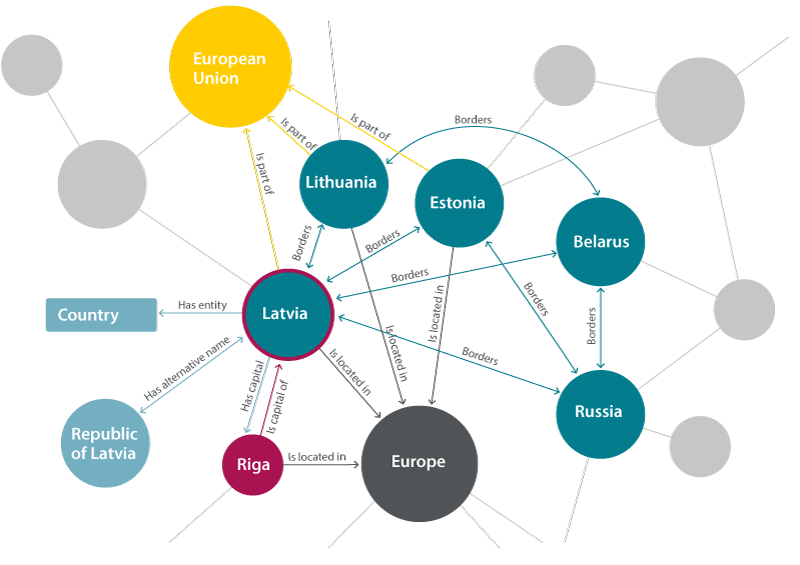
\includegraphics[width=.9\linewidth]{figures/kg-example.png}
 \captionsetup{width=.9\linewidth}
 \caption{An example of a knowledge graph representing how countries are related geographically.}
 \label{fig:kg-example}
\end{wrapfigure}

For example, on the figure~\ref{fig:kg-example}, we could imagine that geographical links (e.g. borders, is located in, \dots) come from a different source (e.g. OpenStreeMap) of information than the political links (e.g. is part of, has alternative name, \dots). In this enhanced graph combining information, two entities might be closer to each other (in terms of graph hops) than in any of the individual sources. \\

Finally, any algorithmic technique employed downstream could potentially make use of the edge type (e.g. borders, is part of, \dots) in the procedure, by giving more weights to specific edge types, for example. All in all, this allows for a much wider spread of potential techniques and information extraction algorithms or models. \\

For these reasons, representing and leveraging knowledge as such has a long history in machine learning and computer science as a whole~\cite{Minsky:1974:FRK:889222, Davis1993WhatIA}. In the last few years, this concept has gained a lot of traction in the scientific community as well as in the industry~\cite{LiuZhiyuan:247, 7358050} for obvious reasons. Indeed, the tremendous progress made in machine learning coupled with this idea of knowledge graph has been applied to many applications such as fraud detection (e.g. for a bank), community identification (e.g. in a social network), recommender systems (e.g. for an online shop). In such systems, it may be difficult for a human to make sense of the different links between entities and how their properties correlate as these links could be multiple hops away from each other. \\

In these previous examples, the entities, properties and relationships could be the following:
\paragraph{Bank knowledge graph: }
\begin{itemize}
 \item[] Entities and Properties:
 \begin{itemize}
  \item Person(First name, Last name, Address)
  \item Company(Name, Address)
  \item Account(Number, Type, Amount)
 \end{itemize}
 \item[] Relationships:
 \begin{itemize}
  \item Person -- \textit{is owner} -- Account
  \item Company -- \textit{is owner} -- Account
  \item Person -- \textit{work at} -- Company
  \item Account -- \textit{wire transfer} -- Account
 \end{itemize}
\end{itemize}
\paragraph{Social network knowledge graph: }
\begin{itemize}
 \item[] Entities and Properties:
 \begin{itemize}
  \item Person(First name, Last name)
  \item Group(Name)
  \item Content(Title)
 \end{itemize}
 \item[] Relationships:
 \begin{itemize}
  \item Person -- \textit{friend with} -- Person
  \item Person -- \textit{likes} -- Content
  \item Person -- \textit{belongs to} -- Group
 \end{itemize}
\end{itemize}
\paragraph{Online shop knowledge graph (figure~\ref{fig:kg-online-shop}): }
\begin{itemize}
 \item[] Entities and Properties:
 \begin{itemize}
  \item Client(First name, Last name)
  \item Category(Name)
  \item Product(Name, Price, Properties)
 \end{itemize}
 \item[] Relationships:
 \begin{itemize}
  \item Client -- \textit{purchased} -- Product
  \item Client -- \textit{follows} -- Category
  \item Product -- \textit{belongs to} -- Category
  \item Product -- \textit{shares property} -- Product
  \item Product -- \textit{has similar price} -- Product
 \end{itemize}
\end{itemize}

\newpage
\begin{figure}
	\centering
	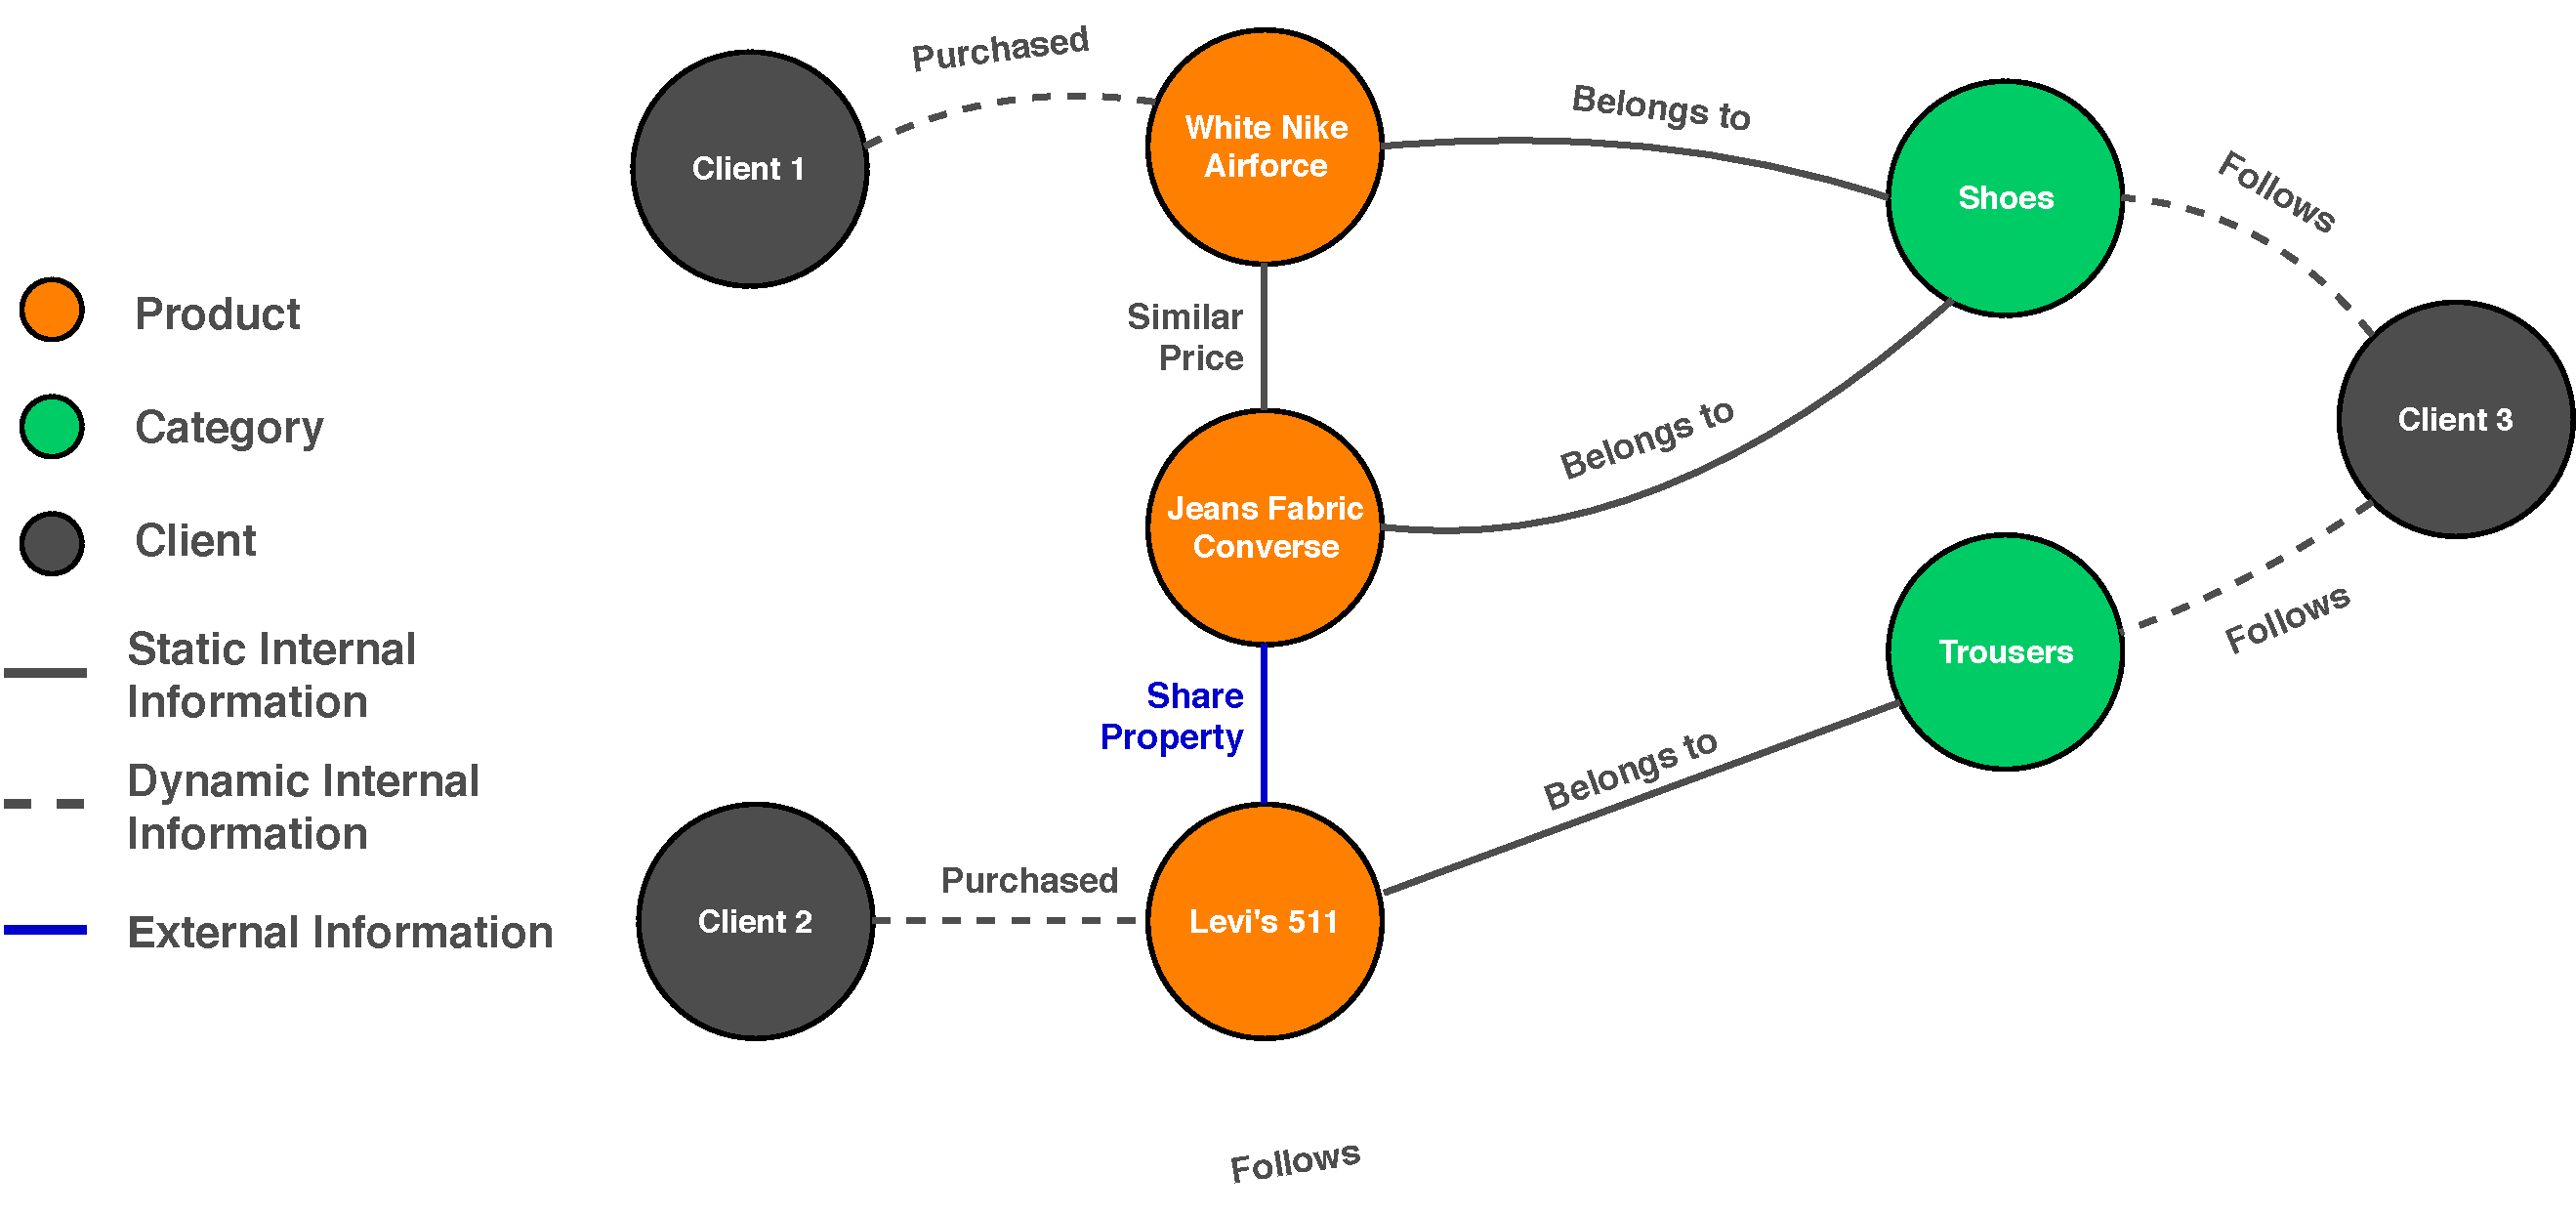
\includegraphics[width=.75\linewidth]{figures/kg-online-shop.pdf}
	\caption{
		An example of evolving knowledge graph for the ``Online Shop`` case described above. The evolution of the graph is shown through the labels $T=t$ for some edges. Indeed, the clients are buying, and generally performing actions, over time and the structure of the graph is evolving accordingly at different time step. The external information linking these \textit{Converse} shoes (made with jeans fabric) and a \textit{Levi's 511} may come from an external database to automatically map product identifiers to materials and fabrics they are made of.
	}
	\label{fig:kg-online-shop}
\end{figure}

\section{Recurrent Neural Network}
\label{sec:Recurrent Neural Network}
Recurrent Neural Network consists of a type of architecture for Deep Learning models that allows exploiting temporal dynamic behavior for sequence. This makes them particularly interesting and efficient for tasks that exhibit a temporal pattern, such as speech recognition or market forecasting. On top of that, this kind of architecture allows processing variable-length sequence input, which is not the case for most of the other machine learning (e.g. \textit{linear regression} or \textit{support vector machine}) or deep learning techniques (e.g. \textit{convolutional neural networks}).\\

Originally, these Recurrent Neural Networks were first heard of in 1986~\cite{10008954896} but the term \emph{recurrent} was not yet used to qualify the progress introduced in the paper. It is only three years later~\cite{6796948} that the term started to appear more actively in the research literature to qualify this type of neural networks. \\

At core of Recurrent Neural Networks, there are cells that rule how information is blended together from previous time steps and current step, and how much importance is given to these past and present steps. Technically, the RNN handles variable-length inputs by storing a hidden state that is recurrently updated at each time step based on its previous hidden state at time \emph{T-1}, and the current input at time \emph{T}. More formally, given a sequence of inputs $\bm{x} = (\bm{x}_1, \bm{x}_2, ..., \bm{x}_T)$, the hidden state $\bm{h}_t$ is updated following the equation:

\begin{equation}\label{eq:rnn_hidden}
\bm{h}_t = 
\begin{cases}
\bm{0}, & t=0 \\
f(\bm{h}_{t-1}, \bm{x}_t; \bm{\theta}), & \mbox{otherwise}
\end{cases}
\end{equation}

With \emph{f} refers to a non-linear function depending on some parameters $\bm{\theta}$. Typically, the equation~\ref{eq:rnn_hidden} is defined as:

\begin{equation}
 \bm{h}_t = f(U\bm{x}_t + W\bm{h}_{t-1} + \bm{b})
\end{equation}

Where the parameters $\bm{\theta}$ are the matrices \emph{W}, \emph{U} and the bias term $\bm{b}$, while the function \emph{f} is a smooth and bounded function such as sigmoid or a hyperbolic tangent. Finally, the sequence of outputs of the RNN $\bm{y} = (\bm{y}_1, \bm{y}_2, ..., \bm{y}_T)$ is usually defined as:

\begin{equation}
\bm{y}_t = g(V\bm{h}_t + \bm{c})
\end{equation}

Where the matrix \emph{V} and the bias vector $\bm{c}$ are learned parameters, while the function \emph{g} is often a \emph{softmax}. \\

Unfortunately, such networks are suffering from many problems while training to use \emph{back-propagation through time} or (\emph{BPTT}). Indeed, this architecture has difficulties capturing long-term dependencies in the input sequence because the gradient update has a tendency to take abnormally big values (i.e. explode) or small ones (i.e.e vanish, since they are squashed at every time steps by the bounded activation functions \emph{sigmoid} or \emph{tanh}). \\

To circumvent these two problems, researchers have designed more sophisticated activation functions, called cell in this case. The two principal types of cell are LSTM~\cite{doi:10.1162/neco.1997.9.8.1735} and GRU~\cite{DBLP:journals/corr/ChoMGBSB14}, the former predating the latter by almost 20 years. A schematic view of these types of cell can be found in~\ref{fig:cells} for a better understanding of the mechanisms ruling the learning dynamic. These are the typical go-to cells for any application requiring a Recurrent Neural Network. However there does not exist a rule of thumb to pick one of the two as this is usually dependent on the application and, more precisely, on the data at hand~\cite{DBLP:journals/corr/ChungGCB14}. Nonetheless, one interesting argument in favor of the GRU cell is that it depends on fewer parameters than LSTM, as they lack an output gate. It makes them particularly interesting when the computational resources are limited or when one wants to iterate over quick experiments. \\

\begin{figure}
 \centering
 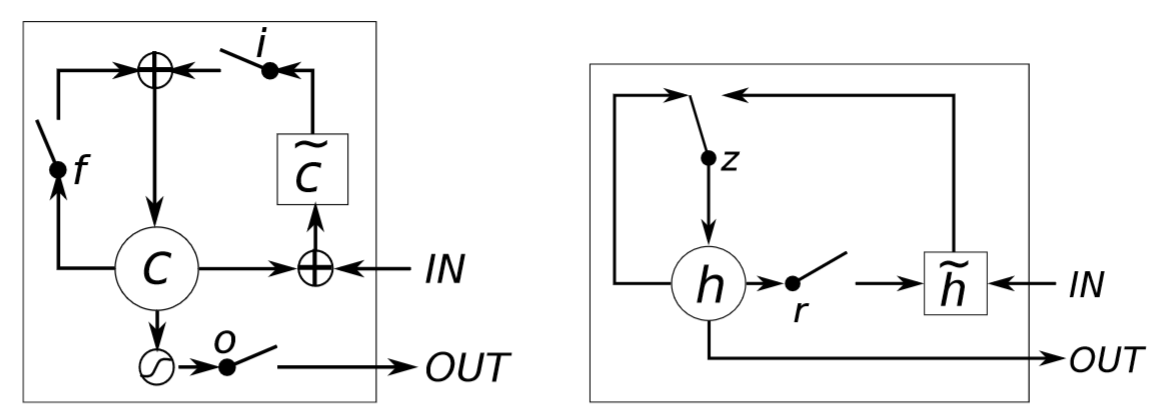
\includegraphics[width=.6\linewidth]{figures/rnn-cells.png}
 \captionsetup{width=.75\linewidth}
 \caption{
  The schematic views of an LSTM (\textit{left}) and GRU (\textit{right}) cell. On the left-hand cell, \emph{i}, \emph{o} and \emph{f} mean respectively \emph{input}, \emph{output} and \emph{forget} gates. Finally, on this same cell, \emph{c} and \emph{$\tilde{c}$} represents the old and new contents of the memory cell. For the right-hand cell, \emph{r} and \emph{z} are the reset and update gates while \emph{h} and \emph{$\tilde{h}$} are respectively the actual and new (or candidate) activation. Figure from~\cite{DBLP:journals/corr/ChungGCB14}.
 }
 \label{fig:cells}
\end{figure}

The equations defining the update dynamics of the hidden state, as well as the other parameters in these cells are the following:

\begin{multicols}{2}
 \centering
 \textbf{LSTM update equations}
 \begin{equation*}
  \begin{aligned}
   \bm{i}_t &= \sigma(U^i\bm{x}_t + W^i\bm{h}_{t-1}) \\
   \bm{f}_t &= \sigma(U^f\bm{x}_t + W^f\bm{h}_{t-1}) \\
   \bm{o}_t &= \sigma(U^o\bm{x}_t + W^o\bm{h}_{t-1}) \\
   \bm{\tilde{C}}_t &= tanh(U^g\bm{x}_t + W^g\bm{h}_{t-1}) \\
   \bm{C}_t &= \sigma(\bm{f}_t \odot \bm{x}_t + \bm{i}_t \odot \bm{\tilde{C}}_t) \\
   \bm{h}_t &= tanh(\bm{C}_t) \odot \bm{o}_t
  \end{aligned}
 \end{equation*}\columnbreak
 \vfill
 \textbf{GRU update equations}
 \begin{equation*}
  \begin{aligned}
   \bm{z}_t &= \sigma(U^z\bm{x}_t + W^z\bm{h}_{t-1}) \\
   \bm{r}_t &= \sigma(U^r\bm{x}_t + W^r\bm{h}_{t-1}) \\
   \bm{\tilde{h}}_t &= tanh(U^h\bm{x}_t + W^h(\bm{r}_t \odot \bm{h}_{t-1})) \\
   \bm{h}_t &= (1-\bm{z}_t) \odot \bm{h}_{t-1} + \bm{z}_t \odot \bm{\tilde{h}}_t
  \end{aligned}
 \end{equation*}
\end{multicols}

Finally, these two cells and all these equations are defining a \emph{causal} structure. That is, the output at time \emph{T} only depends and capture information from the past $1, ..., T-1$ through the learning dynamics. However, it may be interesting to have the output at each time step to \emph{depend on the whole sequence}, in applications where it makes sense. Indeed, if one is doing part-of-speech tagging, the tag of a given work not only depends on the preceding words but following ones. On the contrary, if one wants to run the model on an \textit{online} stream of data for example, it would be flawed to train the model with access to future time steps. \\

However, in many cases it is possible to train such models with information from previous and next states where the relevant architecture is called \emph{Bidirectional RNN}. This kind of model combines an RNN that moves forward and one that moves backward, to finally mix their respective output with a concatenation followed by a fully-connected layer. \\

To conduct our research, we picked GRU cells in our case for the reasons mentioned above, namely their efficiency that allows to iterate over different architectures and hyper-parameters faster. The use of bidirectional RNN or not will be a hyper-parameter tuned with the other ones.

\section{Evolving Knowledge Graph}
\label{sec:Evolving Knowledge Graph}
This last core concept tackles the problem of evolving knowledge graph, where the term \emph{evolving} refers to a dynamic component within the knowledge graph. Furthermore, it characterizes changes in the graphs that can be two fold: changes in the structure (e.g. new entities and links, such as a new \emph{company} in the ``Bank knowledge graph`` example in section~\ref{sec:Knowledge Graph}), changes in properties within entities (e.g. the \emph{product price} could evolve over time for the ``Online shop knowledge graph``). \\

Ultimately, the goal is to account for such dynamic behavior in the structure of the graph or its properties. Indeed, one could consider these changes as a sequence of graph states, each state representing the graph structure and property values at a given time \emph{T}. This additional information would benefit many applications and allow for much complex information interaction than a knowledge graph that remains static. However, incorporating temporal information into knowledge graph-based learning is still one of the major difficulties~\cite{LiuZhiyuan:247}. For this reason, a lot of efforts have been carried around the topic~\cite{D16-1260, 7527876, DBLP:journals/corr/TrivediDWS17, 8047276}, but there still remains a lot of challenges such as scalability to large real-world applications and capacity to capture dynamics in skewed graphs~\cite{DBLP:journals/corr/abs-1812-02289}. \\

With this in mind, we are seeking an architecture that is able to reason over time by capturing the different dynamics of the knowledge graph at the same time as leveraging its structure and relationships. 

\chapter{Healthcare Application \& Dataset}
\label{chap:Dataset}
This chapter will provide the reader with relevant information about the dataset at hand. Indeed, the idea of our approach, \emph{KG-RNN}, is quite general but we demonstrate its usefulness in a concrete application in this thesis. \\

In particular, we develop the concept of \emph{Enhanced Healthcare} and apply our technique to the diagnosis of disease at a patient discharge. To sum up the structure of chapter, we will introduce the dataset in section~\ref{sec:Description}, its source as well as its limitation and scope. Besides, we will explain the preparation procedure of the dataset in section~\ref{sec:Preparation}, how we are processing it and formatting it to be ready for modeling. Finally, we will describe and present statistics about the dataset in section~\ref{sec:Statistics} in order for the reader to have a better grasp of the big picture, the distributions and possibilities offered. \\

All of this bearing in mind our end goal: \textbf{Predict the one or multiple diagnoses assigned to a patient at discharge, among the top-50 most popular ones, given the different events occurring for this patient (measurements, medication, \dots).}

\section{Description}
\label{sec:Description}
To tackle our task of enhancing and improving healthcare by predicting diagnoses of patients at discharge of their ICU stay, we decided to utilize the MIMIC-III dataset~\footnote{\url{https://mimic.physionet.org/}}. This dataset includes over 40 thousand patients with multiple admissions per patient, making for a bit less than 60 thousand in total. All the information is de-identified and subject to restricted database, requiring going through a training program before being able to download any file. All in all, the data spans from June 2001 to October 2012. \\

As a high level, the main component of the dataset is \textit{admissions}; additionally other tables provide information about the different measurements taken throughout a patient time span as well as prescribed drugs. Finally, we are given the diagnoses at discharge, that is both diseases and procedures for the patient. \\

These diagnoses at discharge are represented in the form of ICD9 (\textit{International Classification of Diseases}) codes, which are maintained by the World Health Organization. The purpose of the system is to create a mapping between conditions and generic categories, with different levels of granularity. Indeed, this classification forms a tree where upper-level branches are including the set of similar diseases with specific variations. \\

\newpage
A database of all the ICD codes for version 9 (\textit{ICD9}) can be found at~\url{http://www.icd9data.com/} and here are a few examples to get the reader acquainted with the system:

\begin{table}[H]
 \begin{center}
  \begin{tabular}{ l | p{7cm} }
   \textbf{ICD9 code or range} & \textbf{Description} \\ \hline
   001-139 & Infectious and Parasitic Diseases. \\ \hline
   010-018 & Tuberculosis. \\ \hline
   011 & Pulmonary tuberculosis. \\ \hline
   011.0 & Tuberculosis of lung infiltrative. \\ \hline
   011.03 & Tuberculosis of lung, infiltrative, tubercle bacilli found (in sputum) by microscopy. \\
   \hline
  \end{tabular}
 \end{center}
\end{table}

In the following tables, we will enumerate and describe the different fields available to our research. We filtered these fields and eventually only describe the ones we are using and that is of interest for our application at hand but many more are available in the \textit{MIMIC-III} dataset. \\

Table containing all the admissions from the different patients:

\begin{table}[H]
 \begin{center}
  \caption{Admissions}
  \begin{tabular}{| l | p{7cm} | c | }
   \hline
   \textbf{Name} & \textbf{Description} & \textbf{Example value} \\ \hline
   SUBJECT\_ID &  Unique identifier for the patient. & 23 \\ \hline
   HADM\_ID & Unique identifier for the admission. & 124321 \\ \hline
   ADMITTIME & Time at which the patient was admitted to the hospital. & 2157-10-18 19:34:00 \\ \hline
   DISCHTIME & Time at which the patient was discharged from the hospital. & 2157-10-25 14:00:00 \\ \hline
   DIAGNOSIS & Preliminary, free text diagnosis for the patient on hospital admission. & BRAIN MASS \\
   \hline
  \end{tabular}
 \end{center}
\end{table}

Table containing the different ICD9 codes diagnosed at discharge of the ICU stay:

\begin{table}[H]
 \begin{center}
  \caption{Diagnoses}
  \begin{tabular}{| l | p{7cm} | c | }
   \hline
   \textbf{Name} & \textbf{Description} & \textbf{Example value} \\ \hline
   SUBJECT\_ID &  Unique identifier for the patient. & 62641 \\ \hline
   HADM\_ID & Unique identifier for the admission. & 154460 \\ \hline
   ICD9\_CODE & Diagnoses assigned to the patient at discharge for a given admission. & 3404 \\ \hline
   SEQ\_NUM & Priority number of the given ICD9 code for the patient's admission. & 3 \\
   \hline
  \end{tabular}
 \end{center}
\end{table}

\newpage
Table containing the different laboratory measurements on a patient during his stay at the ICU:

\begin{table}[H]
 \begin{center}
  \caption{Laboratory measurements}
  \begin{tabular}{| l | p{7cm} | c | }
   \hline
   \textbf{Name} & \textbf{Description} & \textbf{Example value} \\ \hline
   SUBJECT\_ID &  Unique identifier for the patient. & 3 \\ \hline
   HADM\_ID & Unique identifier for the admission. & 145834 \\ \hline
   ITEMID & Unique identifier for the measurement type in the database. & 50868 (\textit{Bicarbonate}) \\ \hline
   CHARTTIME & Time at which the observation was charted. & 2101-10-20 16:40:00 \\ \hline
   VALUENUM & Value measured for the specific measure \textit{ITEMID}. & 17.0 \\ \hline
   VALUEUOM & Unit of measurement for the measure \textit{ITEMID}. & mEq/L \\
   \hline
  \end{tabular}
 \end{center}
\end{table}

Table containing the different input fluids administered to a patient during his stay at the ICU:

\begin{table}[H]
 \begin{center}
  \caption{Input events from CareVue (Electronic Medical Records system)}
  \begin{tabular}{| l | p{7cm} | c | }
   \hline
   \textbf{Name} & \textbf{Description} & \textbf{Example value} \\ \hline
   SUBJECT\_ID &  Unique identifier for the patient. & 24457 \\ \hline
   HADM\_ID & Unique identifier for the admission. & 184834 \\ \hline
   ITEMID & Unique identifier for the fluid type in the database. & 30056 (\textit{Po Intake}) \\ \hline
   CHARTTIME & Time at which the observation was charted. & 2193-09-11 09:00:00 \\ \hline
   AMOUNT & Amount of the drug or substance administered \textit{ITEMID}. & 100.0 \\ \hline
   AMOUNTUOM & Unit of measurement of the drug or substance administered \textit{ITEMID}. & ml \\
   \hline
  \end{tabular}
 \end{center}
\end{table}

Table containing the different input fluids administered to a patient during his stay at the ICU:

\begin{table}[H]
 \begin{center}
  \caption{Input events from Metavision (Electronic Medical Records system)}
  \begin{tabular}{| l | p{7cm} | c | }
   \hline
   \textbf{Name} & \textbf{Description} & \textbf{Example value} \\ \hline
   SUBJECT\_ID &  Unique identifier for the patient. & 27063 \\ \hline
   HADM\_ID & Unique identifier for the admission. & 139787 \\ \hline
   ITEMID & Unique identifier for the fluid type in the database. & 225944 (\textit{Sterile Water}) \\ \hline
   STARTTIME & Start time of the injection. & 2133-02-05 05:34:00 \\ \hline
   ENDTIME & End time of the injection. & 2133-02-05 06:30:00 \\ \hline
   AMOUNT & Amount of the drug or substance administered \textit{ITEMID}. & 100.120008 \\ \hline
   AMOUNTUOM & Unit of measurement of the drug or substance administered \textit{ITEMID}. & ml \\ \hline
   RATE & Rate at which the drug or substance \textit{ITEMID} was administered. & 30.036002 \\ \hline
   RATEUOM & Unit of measurement of the rate at which the drug or substance \textit{ITEMID} was administered. & ml/hour \\
   \hline
  \end{tabular}
 \end{center}
\end{table}

\newpage
Table containing the different output fluids measured from a patient during his stay at the ICU:

\begin{table}[H]
 \begin{center}
  \caption{Output events from CareVue and Metavision}
  \begin{tabular}{| l | p{5cm} | c | }
   \hline
   \textbf{Name} & \textbf{Description} & \textbf{Example value} \\ \hline
   SUBJECT\_ID &  Unique identifier for the patient. & 21219 \\ \hline
   HADM\_ID & Unique identifier for the admission. & 177991 \\ \hline
   ITEMID & Unique identifier for the fluid type in the database. & 40055 (\textit{Urine Out Foley}) \\ \hline
   CHARTTIME & Time at which the output fluid was charted. & 2142-09-08 10:00:00 \\ \hline
   VALUENUM & Value measured for the fluid \textit{ITEMID}. & 200.0 \\ \hline
   VALUEUOM & Unit of measurement for the fluids \textit{ITEMID}. & ml \\
   \hline
  \end{tabular}
 \end{center}
\end{table}

Table containing the different medications prescribed to a patient during his stay at the ICU:

\begin{table}[H]
 \begin{center}
  \caption{Prescriptions}
  \begin{tabular}{| l | p{5cm} | c | }
   \hline
   \textbf{Name} & \textbf{Description} & \textbf{Example value} \\ \hline
   SUBJECT\_ID &  Unique identifier for the patient. & 6 \\ \hline
   HADM\_ID & Unique identifier for the admission. & 107064 \\ \hline
   STARTDATE & Start time of the medication's prescription. & 2175-06-11 00:00:00 \\ \hline
   ENDDATE & End time of the medication's prescription. & 2175-06-13 00:00:00 \\ \hline
   DRUG & Identify the type of drug prescribed in the database. & Warfarin \\ \hline
   DRUG\_VAL\_RX & Amount of the medication prescribed \textit{ITEMID}. & 5 \\ \hline
   DRUG\_UNIT\_RX & Rate at which the medication \textit{ITEMID} was prescribed. & mg \\
   \hline
  \end{tabular}
 \end{center}
\end{table}

\paragraph{Limitation \& Scope}
MIMIC-III is a dataset that is de-identified, as explained briefly in the previous session. That is, we do not have access to many personally identifiable information (\textit{PII}) for the patient for obvious confidentiality reasons. \\

For example, all dates in the dataset have been randomly shifted and are therefore not possible to correlate between patients. This is to protect patient confidentiality and times only make sense to interpret at patient scope. This limitation has implications for any downstream application, such as the impossibility to account for medical trends or discoveries in the course of time. \\

Indeed, some new drugs may be discovered or innovative procedures to cope with a particular disease. On top of that, the differential diagnosis process has probably evolved over the years covered by the \textit{MIMIC-III} (2001-2012) and thus particular events or measurements could lead to additional or new diseases diagnosed at discharge.

\newpage
\section{Preparation}
\label{sec:Preparation}
As any real dataset, MIMIC-III is a bit messy and not perfectly structured and normalized. In the following section, we will introduce the various pre-processing and cleaning applied to the dataset to finally talk about dataset formation. \\

The purpose of this section is to ensure a good understanding of the mechanics of the pipeline as well as full reproducibility of the experiments in chapter~\ref{chap:Experiments}.

\subsection{Pre-processing \& Cleaning}
This subsection will be divided in paragraphs, one for each table described in section~\ref{sec:Description}. Each of these paragraph will contain detailed information regarding the processing and cleaning of this specific data.

\paragraph{Admissions} For this table, we had to simply remove NaN entries that were present.

\paragraph{Diagnoses} For this table, we removed NaN entries that were present but also merged procedures and diseases diagnoses. Finally, for readability, we translated ICD9 codes to their classical representation (from MIMIC-III: \textit{42019} to \textit{420.19}).

\paragraph{Laboratory measurements} For this table, we removed NaN entries that were present, we cleaned the units of measurement to lower-case, removed leading and trailing spaces. Finally, we normalized the units of measurements and their values for the same item.\\

For example, \textit{Testosterone level} is charted as \textit{ng/dl} and \textit{pg/dl}, so we decided to convert all the former to the latter and multiply their respective value by \textit{10}.

\paragraph{Input events from CareVue} For this table, we removed NaN entries that were present, we cleaned the units of measurement to lower-case, removed leading and trailing spaces. Finally, we normalized the units of measurements and their values for the same item. For example, there exists \textit{gtt} and \textit{drop} for the same item, or \textit{g} and \textit{mg}.

\paragraph{Input events from Metavision} For this table, we removed NaN entries that were present, we cleaned the units of measurement to lower-case, removed leading and trailing spaces. Finally, we normalized the units of measurements and their values for the same item. For example, there exists \textit{gtt} and \textit{drop} for the same item, or \textit{g} and \textit{mg}. \\

On top of that, input events in \textit{Metavision} are charted in the form of continuous events. That is, a time range is defined as well as a rate and a total amount. Hence, to normalize the data according to \textit{CareVue}, we converted these ranges to a series of one-time events. To do so, we simply divided the total amount of input fluid provided by the size, we then take the rate at which it is administrated (e.g. 1 ml per hour), and create a series of one-time events of this amount at this rate.

\paragraph{Output events from CareVue and Metavision} For this table, we removed NaN entries that were present, we cleaned the units of measurement to lower-case, removed leading and trailing spaces. Finally, we normalized the units of measurements and their values for the same item. For example, there exists \textit{gtt} and \textit{drop} for the same item, or \textit{g} and \textit{mg}.

\paragraph{Prescriptions} For this table, we removed NaN entries that were present, we cleaned the units of measurement to lower-case, removed leading and trailing spaces. Finally, we normalized the units of measurements and their values for the same item. For example, there exists \textit{gtt} and \textit{drop} for the same item, or \textit{g} and \textit{mg}. \\

Finally, in a similar manner as \textit{input events from Metavision}, prescriptions are charted as daily ratio of drugs that should be taken between two dates. Therefore, we converted these ranges to one-time events of daily doses taken at lunch. \\

After cleaning and processing the different tables, each admission is split in chunks of $\tau$ hours. From there, each chunk contains the events that were charted during that period (laboratory measurements, input events, output events, prescriptions), as a group. \\

These groups/chunks can be seen the patient state at time \emph{T}, this helps deal with all the missing values present in the dataset. Indeed, for the task at hand, we are not interested in the exact value of each patient's vital, but rather by the evolution of his state throughout the admission. To this end, discarding missing values and grouping within a given period makes sense rather than trying to impute missing values, dynamically while training~\cite{Che2018} or upstream.

\newpage
\subsection{Formation}
\label{sec:Formation}
Dataset formation is not a subtle task as this will dictate how downstream models take the data in. This step of the pipeline starts from the previous stage where we cleaned and pre-processed the different tables.\\

To get started, we load the client and pre-processed data from the previous section. From there, we start by splitting the dataset in training, validation and testing sets. To do so, we consider patients instead of admissions as we don't want the same patient to be both in the training and testing sets since a few of them have multiple admissions. Surely, training on one admission and testing on another from the same patient would leak information between training and testing set and thus introduce bias in performance metrics. \\

When the different sets are created, we start by padding or truncating the admissions, depending on whether they are respectively shorter or longer than a pre-defined length. This length $N$ is defined with respect to the number of chunks/groups representing the patient state, so the total admission length considered is computed as $N\tau$. \\

The different admissions are thus padded with zeros, on the left-hand side (so back in time, temporally), which means that for an admission consisting of 3 chunks, or states, $\bm{a_i}=[\bm{c_1}, \bm{c_2}, \bm{c_3}]$, it would be transformed as follows:

\begin{equation*}
\bm{a_i}=[\bm{c_1}, \bm{c_2}, \bm{c_3}] \quad \xrightarrow{\mbox{pad}} \quad \bm{a_i^*}=[\bm{0}, \bm{0}, \dots, \bm{c_1}, \bm{c_2}, \bm{c_3}]\mbox{, where }|\bm{a_i^*}|=N
\end{equation*}

While for a longer admission $\bm{a_i}=[\bm{c_1}, \bm{c_2}, \bm{c_3}, \dots, \bm{c_{178}}]$, we would have:

\begin{equation*}
\bm{a_i}=[\bm{c_1}, \bm{c_2}, \bm{c_3}, \dots, \bm{c_{178}}] \quad \xrightarrow{\mbox{truncate}} \quad \bm{a_i^*}=[\bm{c_1}, \bm{c_2}, \bm{c_3}, \dots, \bm{c_{150}}]
\end{equation*}

On top of this, each chunk is padded and truncated from its events when more than $K$ of them happen within a specific of $c_i$ duration $\tau$. That is, we limit the number of events per $c_i$ in the equations above. Therefore, the events within each chunk are also zero-padded if the number of events is lower than $K$, and randomly sampled if it exceeds $K$.\\

Consequently, we have fixed number of chunks (\textit{admission length}) and fixed number of events per chunk. As a result, we are able to batch the admissions and leverage computational efficiency to reduce the training time, which is the main rational between these truncating and padding procedures. Finally, the packed admissions are cast to \emph{float32} from \emph{float64}, in order to reduce memory footprint at the cost of a very slight decrease in terms of value precision.

\newpage
\subsection{Schematic Visualizations}
The goal of this subsection is to show with a schema the results induced by the previous sections \emph{Pre-processing \& Cleaning} and \emph{Formation}. It is important to note that in these visualizations, input events are only shown in the form of the Metavision system (\textit{input events MV}), as ranges in the input row (\textit{green}). \\

\begin{figure}[H]
 \setkeys{Gin}{width=\linewidth}
 \begin{tabularx}{\textwidth}{XXXX}
  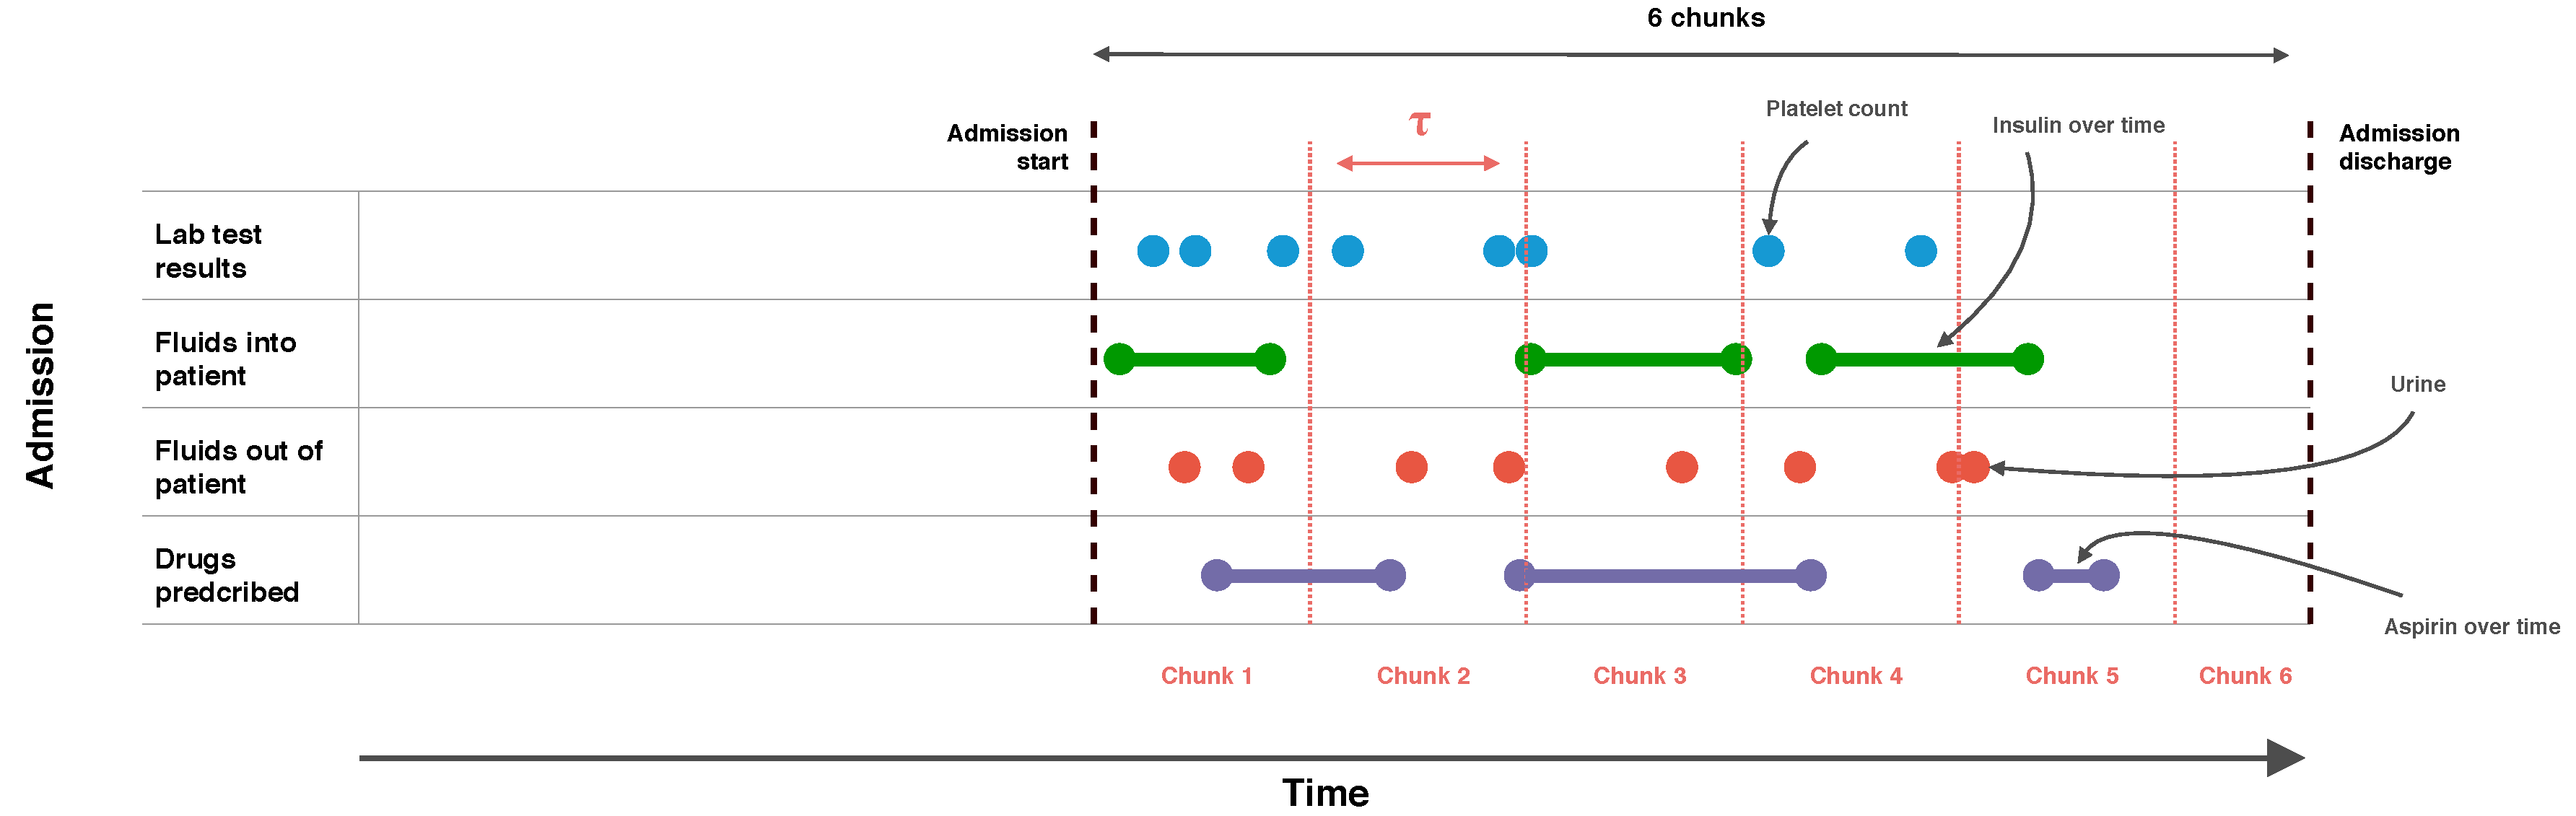
\includegraphics{figures/adm-before.pdf} \\[1.2cm]
  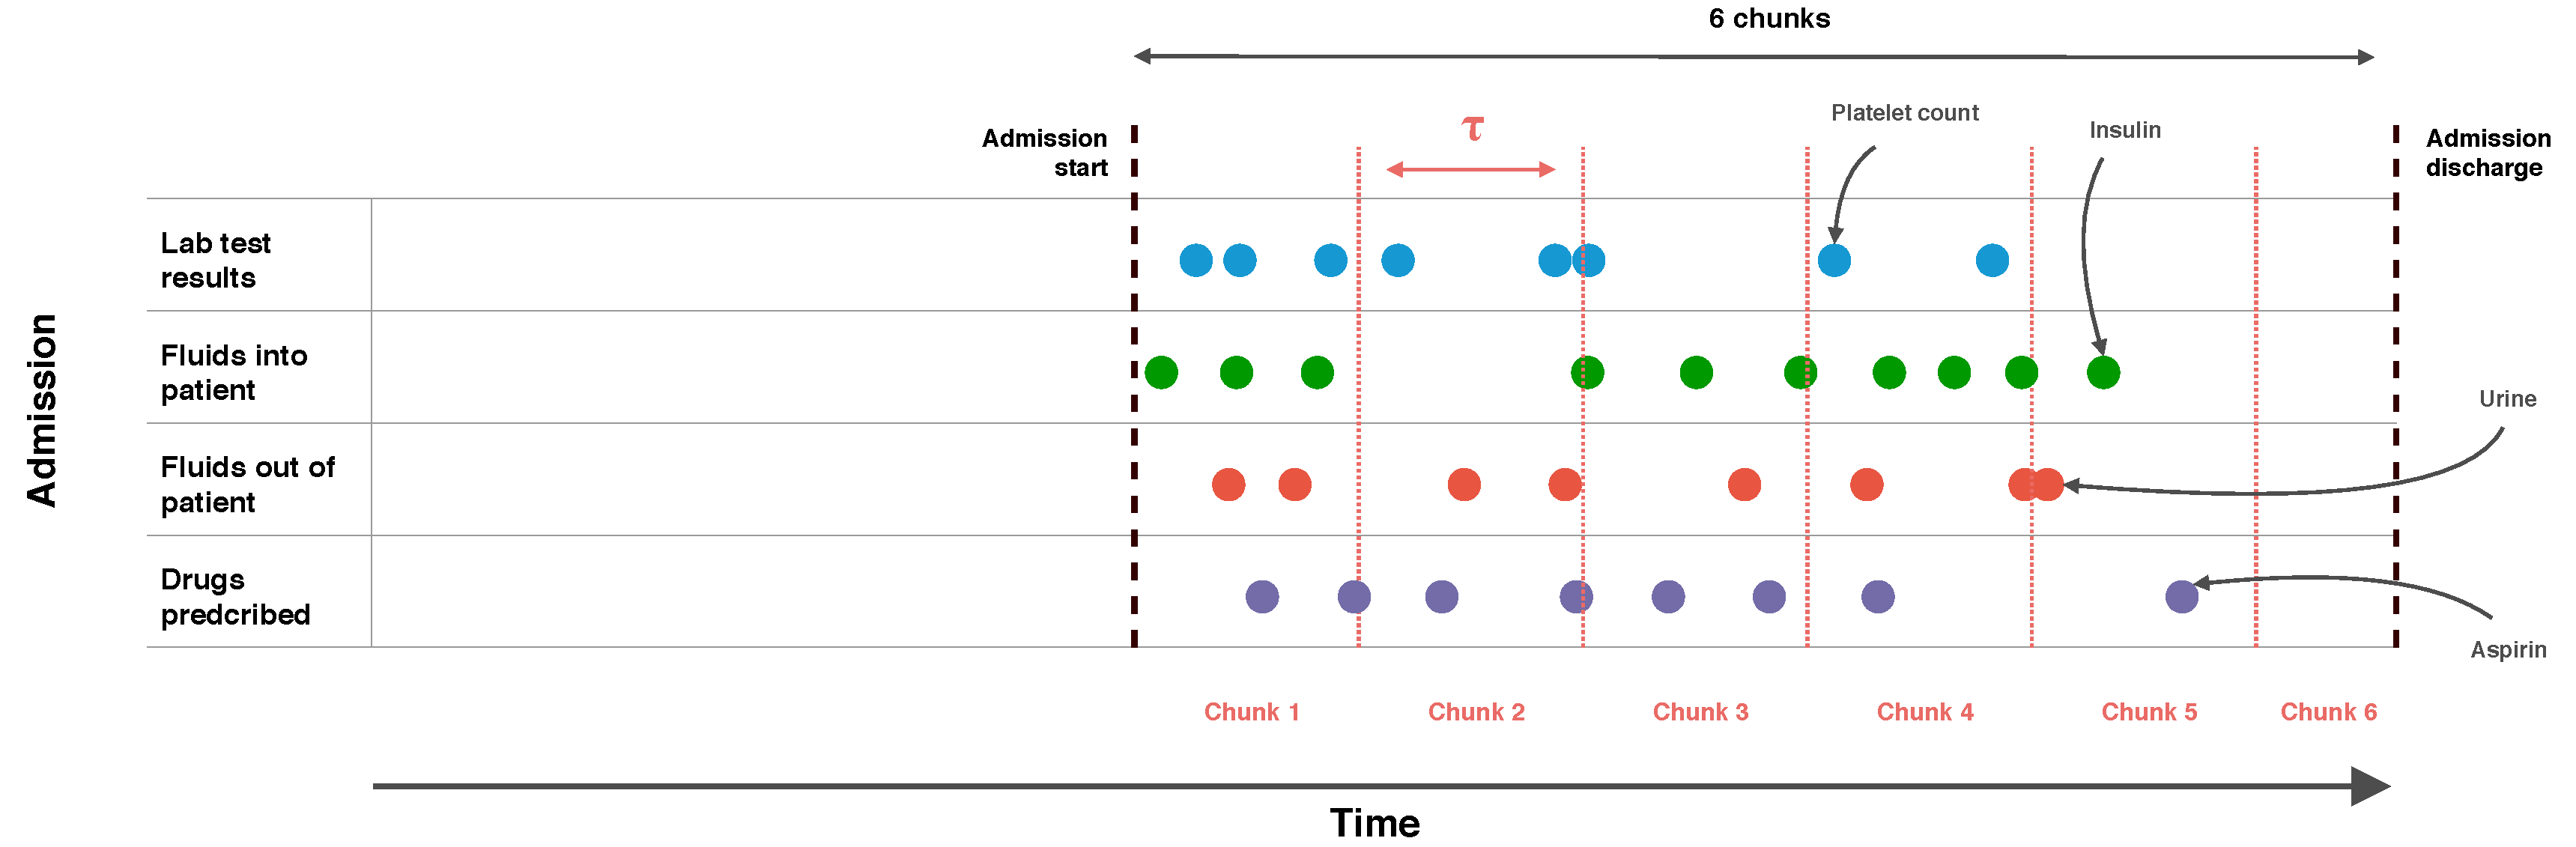
\includegraphics{figures/adm-after-1.pdf} \\[1.2cm]
  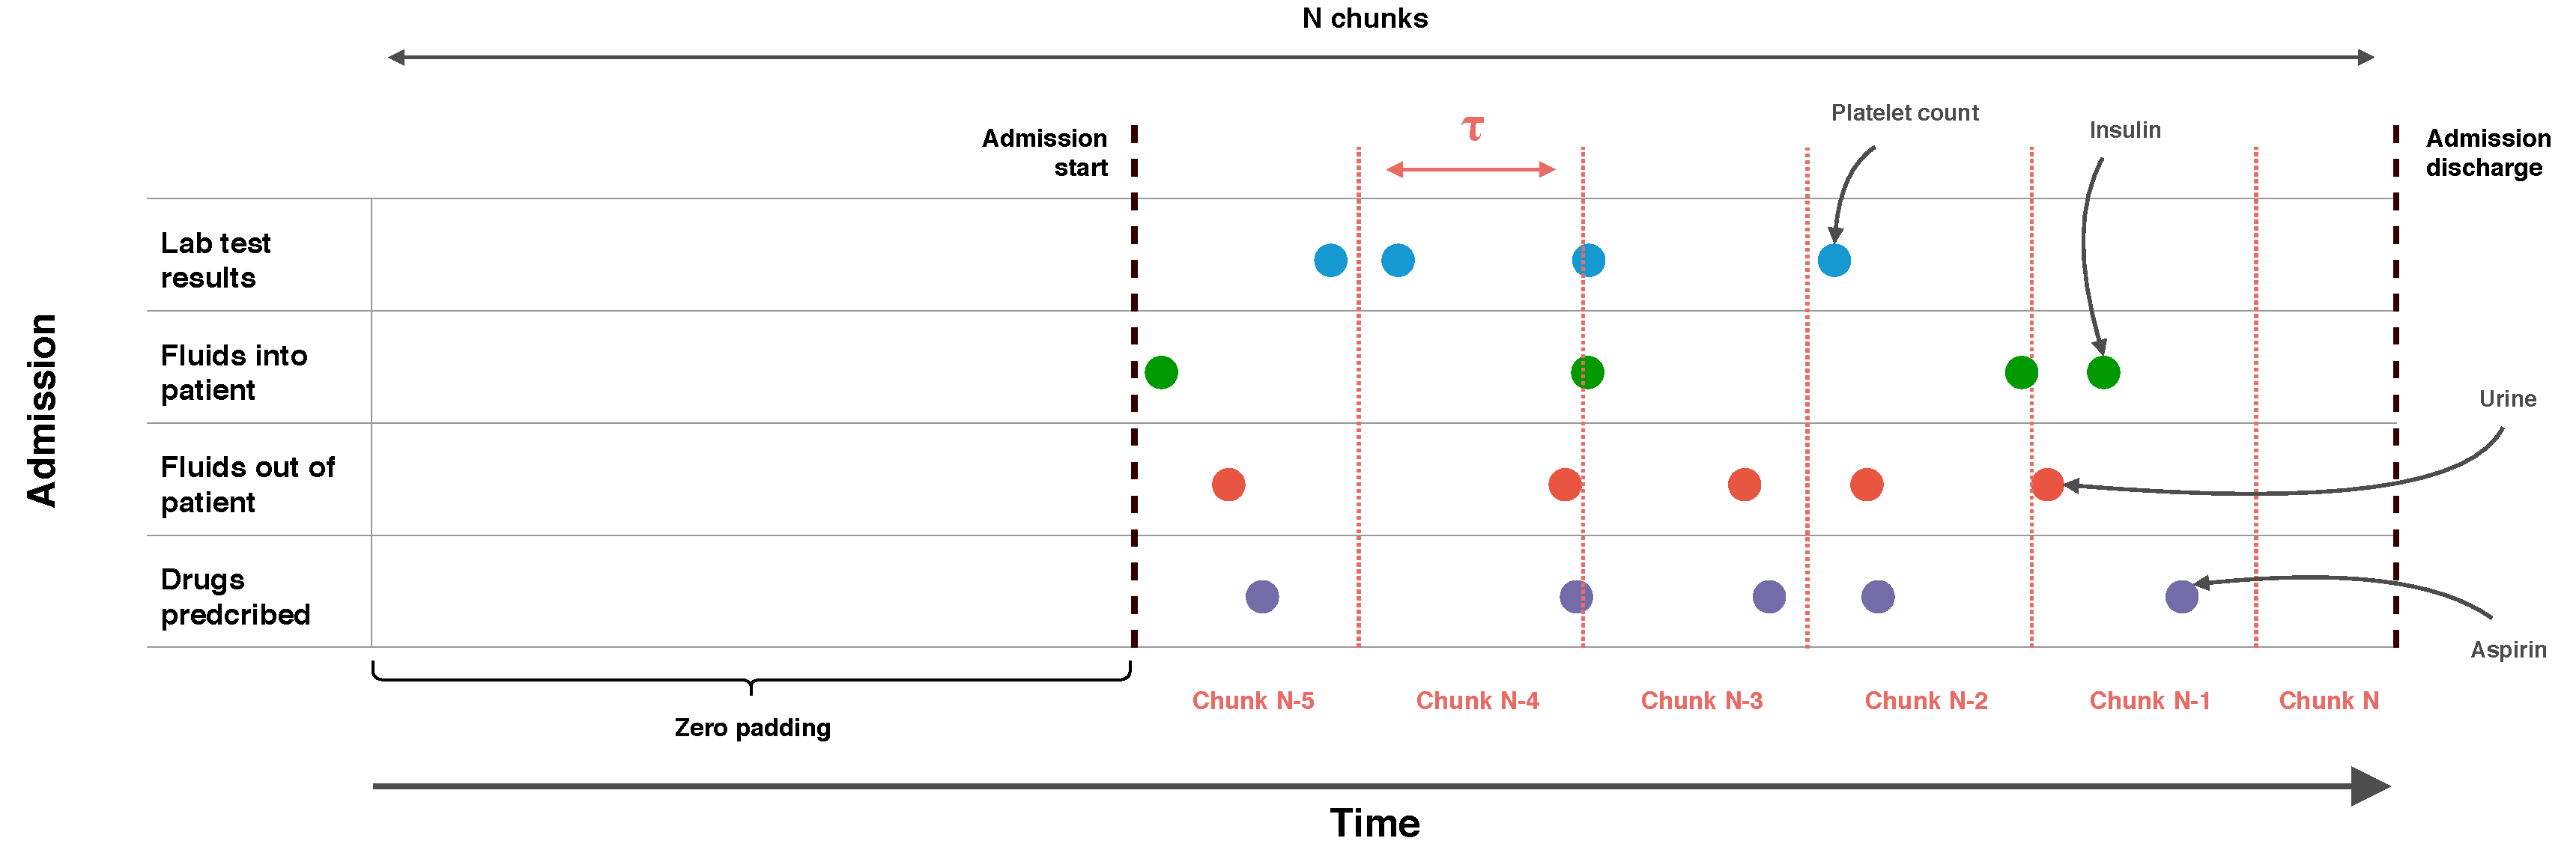
\includegraphics{figures/adm-after-2.pdf}
 \end{tabularx}
 \caption{\textbf{Top row}: The visualization of a single admission, consisting of 6 chunks of duration $\tau$, each with their respective one-time or range events. \textbf{Middle row}: The pre-processed and cleaned admission, range events have been converted to one-time events. \textbf{Bottom row}: The final version of the admission that will be fed to the downstream model. The admission is padded and events are sampled with $K=1$, thus we only have 1 event per type and per chunk of duration $\tau$. Chunks with less than $K=1$ events are also \textit{zero padded} (not shown) to match the $K$ number of events per type and per chunk.}
\end{figure}

\newpage
\section{Statistics}
\label{sec:Statistics}
This section describes the different statistics related to the data we have discussed until now, to give some quantitative metrics. In effect, the reader will be able to grasp the possibilities and distributions.

\begin{table}[H]
 \begin{center}
  \caption{Dataset size and unique values for each table}
  \begin{tabular}{| l | c | c |}
   \hline
   \textbf{Table} & \textbf{Number of events} & \textbf{Number of types} \\ \hline
   Admissions & 58'976 & - \\ \hline
   Laboratory measurements & 19'306'086 & 368 \\ \hline
   Input events CV & 11'651'110 & 2'836 \\ \hline
   Input events MV & 80'393'617 & 165 \\ \hline
   Output events & 4'217'736 & 1'113 \\ \hline
   Prescriptions & 14'728'948 & 4'465 \\ \hline
   Diagnoses & 891'142 & 9'016  \\
   \hline
  \end{tabular}
 \end{center}
\end{table}

Here are some statistics regarding each state/chunk (with $\tau=3\mbox{ hours}$) and the different events happening throughout the admission timeline:

\begin{multicols}{2}
 \centering
 \textbf{Number of chunks}
 \begin{center}
  \begin{tabular}{| l | c |}
   \hline
   \textbf{Statistic} & \textbf{Value} \\ \hline
   Minimum & 1 \\ \hline
   Maximum & 2'358 \\ \hline
   Average & 81.58 \\ \hline
   Median & 52 \\ \hline
   95th percentile & 247 \\ \hline
   99th percentile & 511 \\
   \hline
  \end{tabular}
 \end{center}\columnbreak
 \textbf{Laboratory measurements per chunk}
 \begin{center}
  \begin{tabular}{| l | c |}
   \hline
   \textbf{Statistic} & \textbf{Value} \\ \hline
   Minimum & 0 \\ \hline
   Maximum & 153 \\ \hline
   Average & 3.76 \\ \hline
   Median & 0 \\ \hline
   95th percentile & 25 \\ \hline
   99th percentile & 37 \\
   \hline
  \end{tabular}
 \end{center}
\end{multicols}

\begin{multicols}{2}
\centering
\textbf{Input CV events per chunk}
\begin{center}
 \begin{tabular}{| l | c |}
  \hline
  \textbf{Statistic} & \textbf{Value} \\ \hline
  Minimum & 1 \\ \hline
  Maximum & 189 \\ \hline
  Average & 2.46 \\ \hline
  Median & 0 \\ \hline
  95th percentile & 15 \\ \hline
  99th percentile & 28 \\
  \hline
 \end{tabular}
\end{center}\columnbreak
\textbf{Input MV events per chunk}
\begin{center}
 \begin{tabular}{| l | c |}
  \hline
  \textbf{Statistic} & \textbf{Value} \\ \hline
  Minimum & 0 \\ \hline
  Maximum & 36'400 \\ \hline
  Average & 15.95 \\ \hline
  Median & 0 \\ \hline
  95th percentile & 19 \\ \hline
  99th percentile & 464 \\
  \hline
 \end{tabular}
\end{center}
\end{multicols}

\begin{multicols}{2}
 \centering
 \textbf{Output events per chunk}
 \begin{center}
  \begin{tabular}{| l | c |}
   \hline
   \textbf{Statistic} & \textbf{Value} \\ \hline
   Minimum & 0 \\ \hline
   Maximum & 41 \\ \hline
   Average & 0.89 \\ \hline
   Median & 0 \\ \hline
   95th percentile & 4 \\ \hline
   99th percentile & 7 \\
   \hline
  \end{tabular}
 \end{center}\columnbreak
 \textbf{Prescriptions per chunk}
 \begin{center}
  \begin{tabular}{| l | c |}
   \hline
   \textbf{Statistic} & \textbf{Value} \\ \hline
   Minimum & 0 \\ \hline
   Maximum & 7'321 \\ \hline
   Average & 1.75 \\ \hline
   Median & 0 \\ \hline
   95th percentile & 9 \\ \hline
   99th percentile & 40 \\
   \hline
  \end{tabular}
 \end{center}
\end{multicols}

These different statistics helped us define the hyper-parameters related to the padding or truncation of admissions ($N$) as well as the number of events per chunk ($K$). \\

Finally, we show some plots and histograms to enlighten the reader regarding the task at hand, which is to predict the diagnosed top 50 most frequent ICD9 codes at discharge in a multi-class multi-classification fashion:

\begin{figure}[H]
 \setkeys{Gin}{width=\linewidth}
 \begin{tabularx}{\textwidth}{XXXX}
  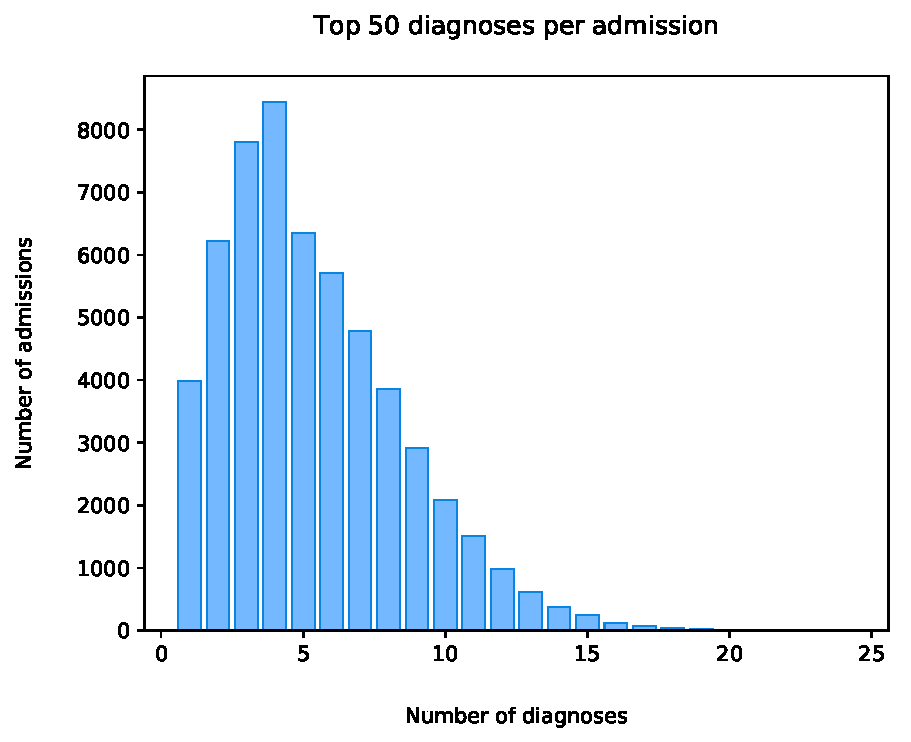
\includegraphics{figures/adm-icd9.pdf} &
  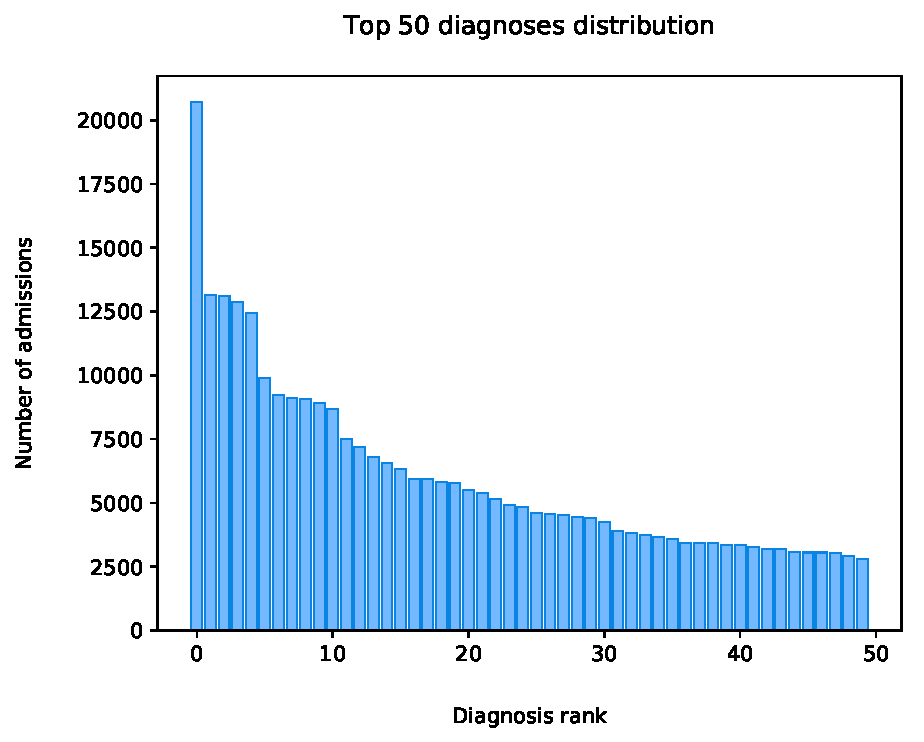
\includegraphics{figures/icd9-top50.pdf} \\
  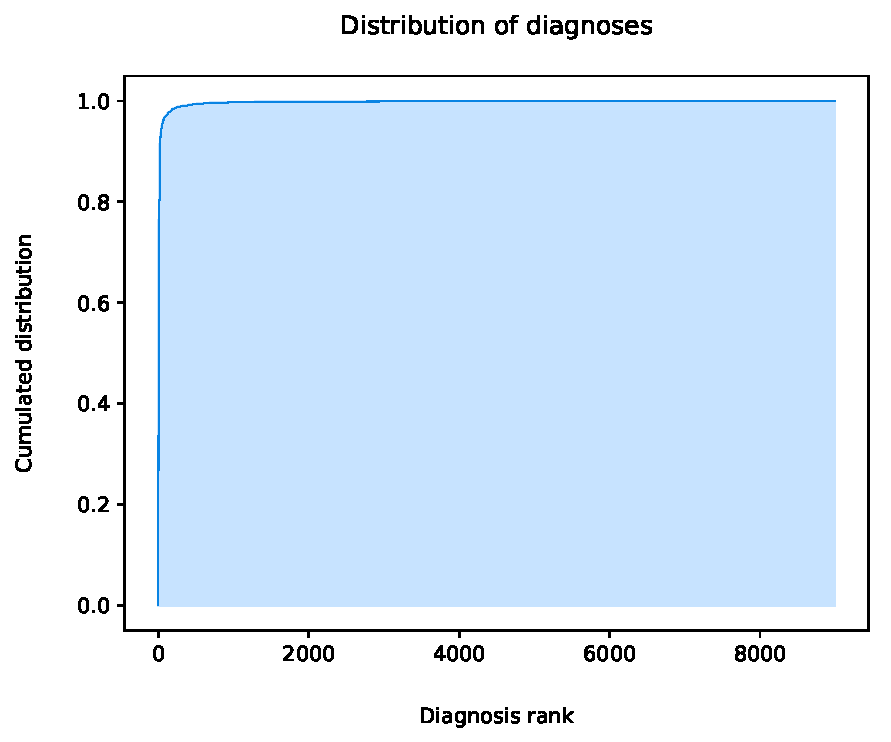
\includegraphics{figures/cdf.pdf} &
  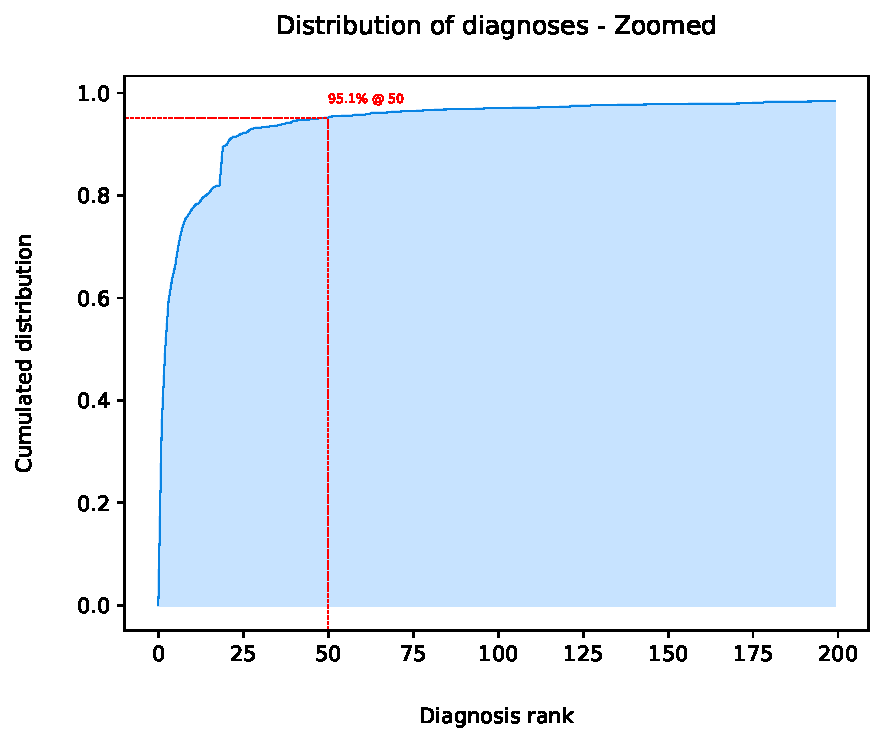
\includegraphics{figures/cdf-200.pdf} \\
 \end{tabularx}

 \caption{\textbf{Top-left}: This histogram represents the number of diagnoses per admission at discharge for the top 50 ICD 9 codes, which is interesting to bear in mind in our setup of multi-class multi-classification. \textbf{Top right}: This histogram represents the number of occurrences among the top 50 diagnoses, this is an indicator of the class imbalance or not. \textbf{Bottom-left}: The cumulative distribution of diagnoses over admissions, we can see that a few diagnoses span more than 90\% of the admissions very rapidly. \textbf{Bottom right}: The zoomed cumulative distribution of diagnoses over admissions, focusing on the top 200 most frequent diagnoses. We can see that we cover 95.1\% of admissions with the top 50 most frequent ICD9 codes.}
 \label{fig:icd9-codes}
\end{figure}
\chapter{Baseline}
\label{chap:Baseline}
This chapter introduces the baseline architecture, which processes an evolving graph. First off, we will go through an overview of the task and a rather ``textual`` description of the model. \\

Then, the baseline model will be described in a more precise way as well as a schematic visualization of the operations that are performed.

\section{Overview}
The baseline architecture deals with the problem of processing a single graph, evolving over time. This graph that will be fed to the downstream model is represented by a series of states.\\

In our case the input entities of interest in our graph are admissions, and the simplest way to predict the diagnoses at discharge of a given input admission is to only consider its events over time as our evolving graph and not directly considering the information from other admission entities. That is, in this baseline approach, we do not consider a knowledge graph linking admissions together within a complex structure, but rather admissions as individual evolving graphs consisted of chunk and event entities. \\

\begin{wrapfigure}{l}{0.5\textwidth}
 \centering
 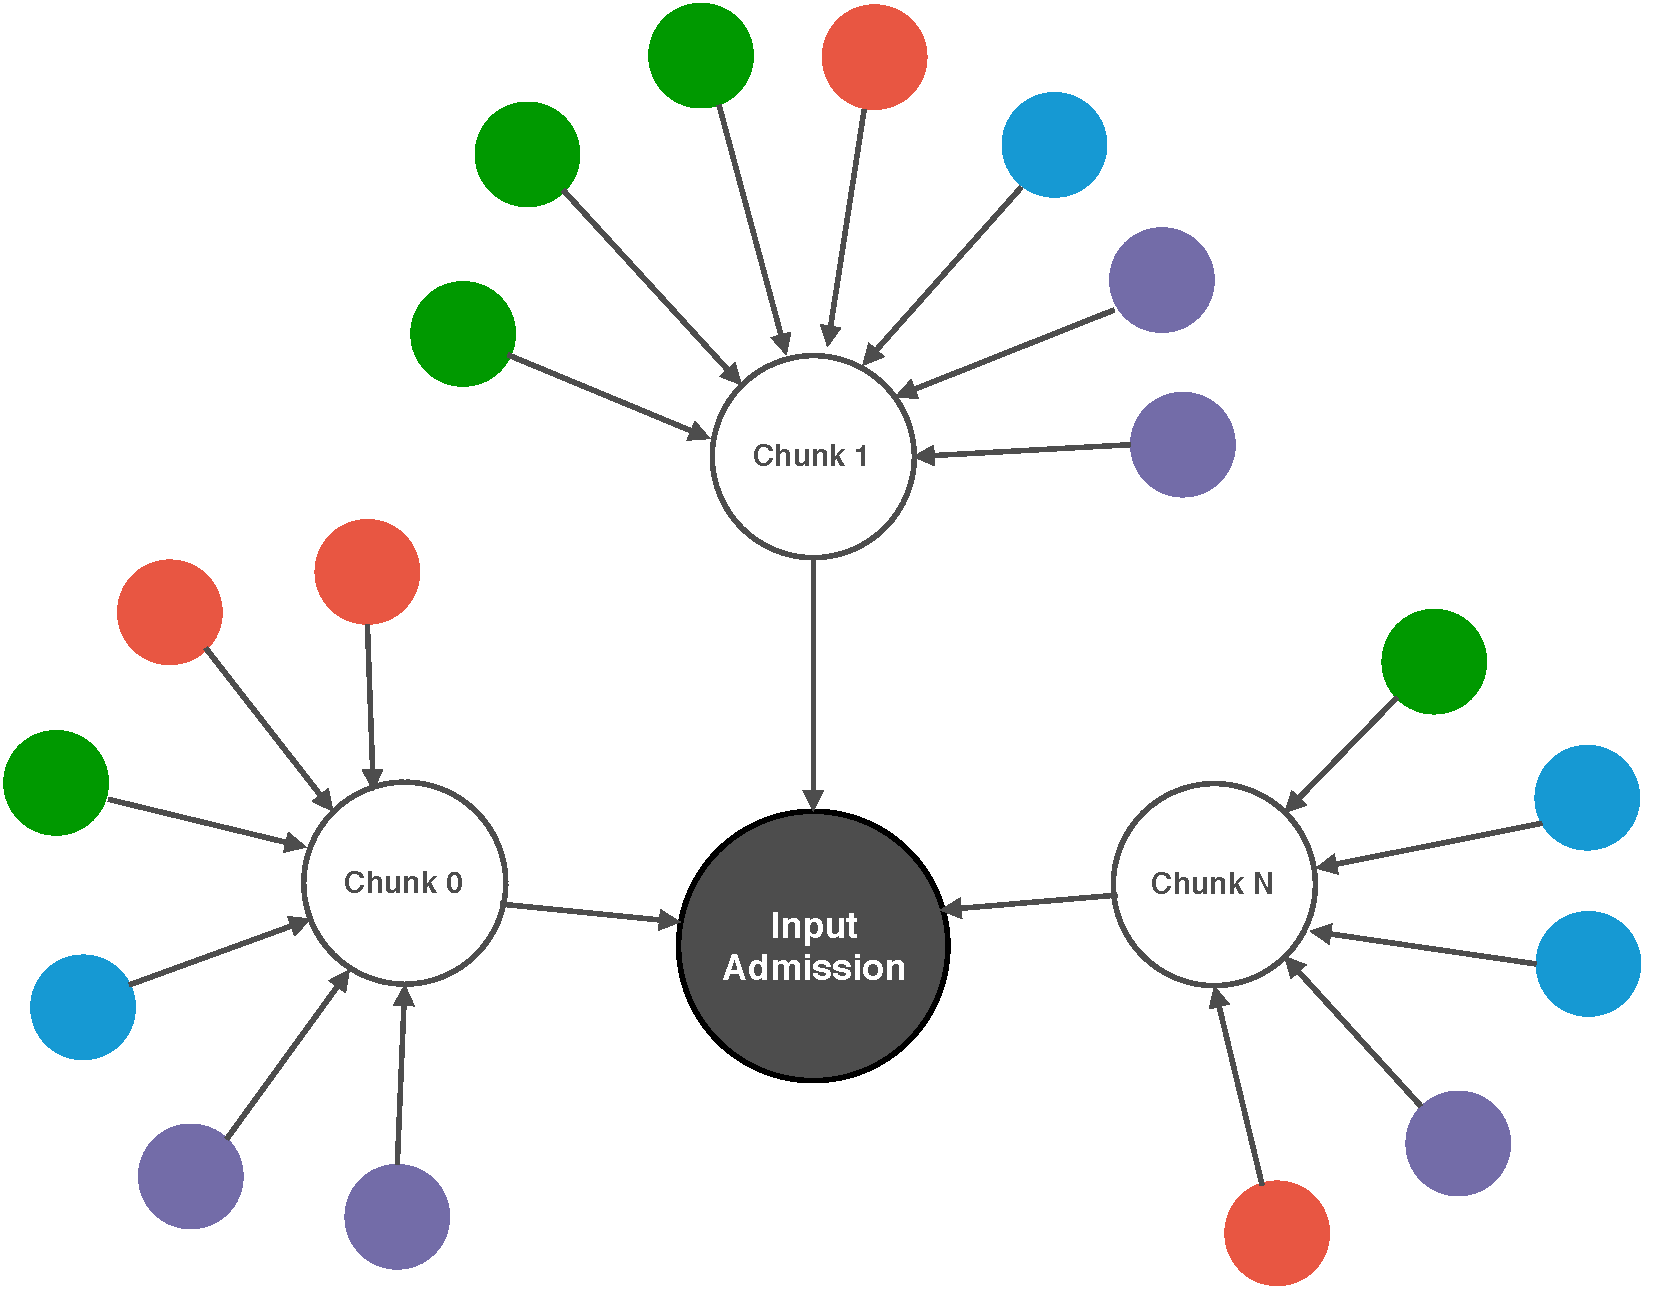
\includegraphics[width=.8\linewidth]{figures/single-adm-graph.pdf}
 \captionsetup{width=.8\linewidth}
 \caption{Example admission (\textit{without} zero padding), where chunk entities have a natural ordering and event entities do not.}
 \label{fig:single-adm-graph}
\end{wrapfigure}

Such a graph can be represented in a compact form as shown in the figure~\ref{fig:single-adm-graph}, the colored entities refer to particular events during the admission timeline, associated to a given chunk depending on the chart time. This admission has a set of diagnoses at discharge and we are looking for an architecture that would enable us to capture the dynamic behavior as well as make sense of the different events. \\

Therefore, it is natural that we base our research and baseline architecture on a Recurrent Neural Network to deal with the different chunks or states of the graph, this type of architecture allowing exploiting temporal dynamic behavior for sequence. Consequently, we need to input an embedded representation of the graph state at every time step $T$ in our Recurrent Neural Network. That is, we need to \textit{map} our graph state into a finite D-dimensional vector (where D is a hyper-parameter to be chosen appropriately) that will enable us to train the model end-to-end. Indeed, as opposed to older techniques that embed the graph in a separate task, making the back-propagation truncated between the RNN and the graph embedding algorithm, we want our architecture to be fully differentiable. \\

\section{Machine Learning Model}
Unlike performing machine learning over classical lattices (e.g. images), the neighboring entities or nodes (i.e. \textit{events}) to our graph states do not have a natural ordering. For this reason, owing to GraphSAGE~\cite{DBLP:journals/corr/HamiltonYL17}, we base our ``graph state embedder`` on aggregator functions for each entity type. These functions must operate over an unordered set of vectors and thus be invariant to permutations of its elements. \\

However, before discussing the aggregator functions in detail, the different events as well as their respective value should be ``translated`` in vector forms. As an illustration, let's consider the following event from the \textbf{Prescriptions table}:

\begin{equation*}
 e^{prescription} = (\mbox{Warfarin}, 5)
\end{equation*}

This tuple represents an entity of the type \emph{prescription event}, where the patient took 5 units of Warfarin. From there, we create a \textbf{prescription embedding matrix} that maps from ``Warfarin`` to a $n$-dimensional vector, where $n$ is a hyper-parameter to be tuned carefully. Finally, this \textbf{prescription embedding matrix}, $M\in\mathbb{R}^{P \times n}$ where $P$ represents the number of prescriptions (4'465 in our case), is initialized with zero-vectors. \\

At the beginning of the training procedure, each prescription event is mapped to its corresponding $n$-dimensional vector and concatenated to its associated value:

\begin{equation*}
\tilde{e}^{prescription} = [\bm{x}, 5]\mbox{, where }\bm{x}\in\mathbb{R}^n
\end{equation*}

At the end of this ``translation`` procedure, each prescription event entity is a $(n+1)$-dimensional vector that can be further processed. In a similar fashion, we create an embedding matrix for each event types, resulting in 5 different embedding matrices initialized with zero-vectors that will allow to ``translate`` every event entities in the evolving graph. \\

Hence, a chunk $i$ can be represented as a tensor of shape $5 \times K \times (n+1)$, resulting from the concatenation of the different event types. Thus, an admission can be seen as a series of chunks, leading to a tensor of shape $N \times 5 \times K \times (n+1)$ for each admission. \\

As mentioned previously, these aggregators should be invariant to permutations of the input, trainable and also have a high representational capacity. To this end, each \textit{aggregator} will first consist of a fully-connected network and followed by the aggregation function, we propose three candidates:

\paragraph{Max aggregator} The first nominee consists in element-wise max-pooling operation along the $K$ dimension. Namely, we have the following end-to-end aggregator:

\begin{equation}
 \label{eq:max_agg}
 \begin{aligned}
 AGG_m^{max} &= \max_{i \in \{0 \dots K\}} \sigma(\bm{W}\bm{\tilde{e}}_i^m + \bm{b})\mbox{, where }\bm{\tilde{e}}_i^m \in \mathbb{R}^{n+1} \\
 &= \max_{i \in \{0 \dots K\}} \bm{h}_i^m\mbox{, where }\bm{h}_i^m \in \mathbb{R}^{a}
 \end{aligned}
\end{equation}

Here $\max$ denotes the element-wise max operator along the $K$ dimension, $\sigma$ is a nonlinear activation function (e.g. ReLU) and $a$ is an arbitrary dimensionality that has to be manually tuned. Besides, $m$ represents the event type among laboratory measurements, input events (CV or MV), output events and prescriptions, while $\bm{W} \in \mathbb{R}^{a \times (n+1)}$ and $\bm{b} \in \mathbb{R}^a $ are parameters optimized during the back-propagation training. \\

All in all, for each event type $m$, the equation~\ref{eq:max_agg} maps each embeddings to a $a$-dimensional hidden representation $\bm{h}_i^m$ and then squashes the events of a similar type with the max operator.

\paragraph{Mean aggregator} This aggregator is very similar to the \textit{max aggregator} but performs a mean-pooling operation along the $K$ dimension:

\begin{equation}
 \label{eq:max_agg}
 \begin{aligned}
  AGG_m^{mean} 
   &= \underset{i \in \{0 \dots K\}}{\mbox{mean}} \sigma(\bm{W}\bm{\tilde{e}}_i^m + \bm{b})\mbox{, where }\bm{\tilde{e}}_i^m \in \mathbb{R}^{n+1} \\
   &= \underset{i \in \{0 \dots K\}}{\mbox{mean}} \bm{h}_i^m\mbox{, where }\bm{h}_i^m \in \mathbb{R}^{a}
 \end{aligned}
\end{equation}

\paragraph{Sum aggregator} Our final candidate looks like the two previous ones, by replacing the element-wise operator with a sum operation:

\begin{equation}
\label{eq:max_agg}
 \begin{aligned}
 AGG_m^{sum} 
  &= \underset{i \in \{0 \dots K\}}{\mbox{sum}} \sigma(\bm{W}\bm{\tilde{e}}_i^m + \bm{b})\mbox{, where }\bm{\tilde{e}}_i^m \in \mathbb{R}^{n+1} \\
  &= \underset{i \in \{0 \dots K\}}{\mbox{sum}} \bm{h}_i^m\mbox{, where }\bm{h}_i^m \in \mathbb{R}^{a}
 \end{aligned}
\end{equation}

A visual explanation is available on the figure~\ref{fig:agg-example}. In essence, it is important to note that all of these aggregators are both symmetric and trainable. Once stacked, the output of these aggregators is a tensor of shape $N \times 5 \times a$ that we further reshape and concatenate to $N \times 5a$ in order to be fed to our downstream Recurrent Neural Network. Thus, referring to the previous section, each $5a=D$ vector is our representation of the graph state at the time step $T$. \\

This Recurrent Neural Network outputs a vector of size $\bm{\tilde{h}} \in \mathbb{R}^{b}$ that is represented the embedding of our \textbf{evolving entity}. In our practical use-case to predict the ICD9 codes at discharge, we simply feed this vector into a fully-connected layer mapping to our \emph{50} classes.\\

More generally, this embedding algorithm followed by a Recurrent Neural Network is applicable to any arbitrary entity and we call it an \textbf{Evolving Entity Encoder}. We present the baseline model applied to our ``Healthcare Dataset`` but it generalizes easily to different graphs and structures, since it is independent of the number of neighbors.

\begin{figure}[h]
 \centering
 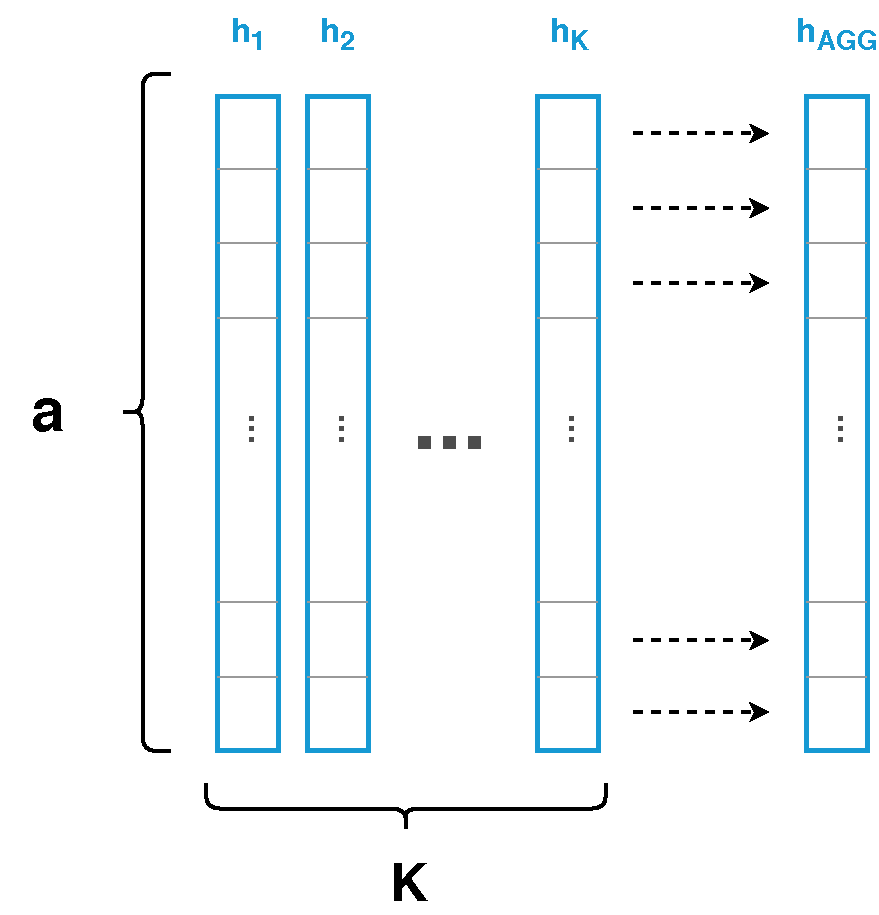
\includegraphics[width=0.35\textwidth]{figures/agg-example.pdf}
 \caption{An example of an aggregator on a certain event type (\textit{blue}), the dashed arrow represent the type of aggregating function (i.e. sum, mean, max) applied element-wise (row-by-row on the figure). The output is a vector $\bm{h}_{AGG} \in \mathbb{R}^{a}$.}
 \label{fig:agg-example}
\end{figure}

\newpage
\begin{landscape}
 \section{Schematic Visualization}
 To better understand how the baseline architecture works and generalizes to arbitrary graphs, we propose the following visualizations to the reader: \\
 
 \begin{figure}[H]
  \centering
  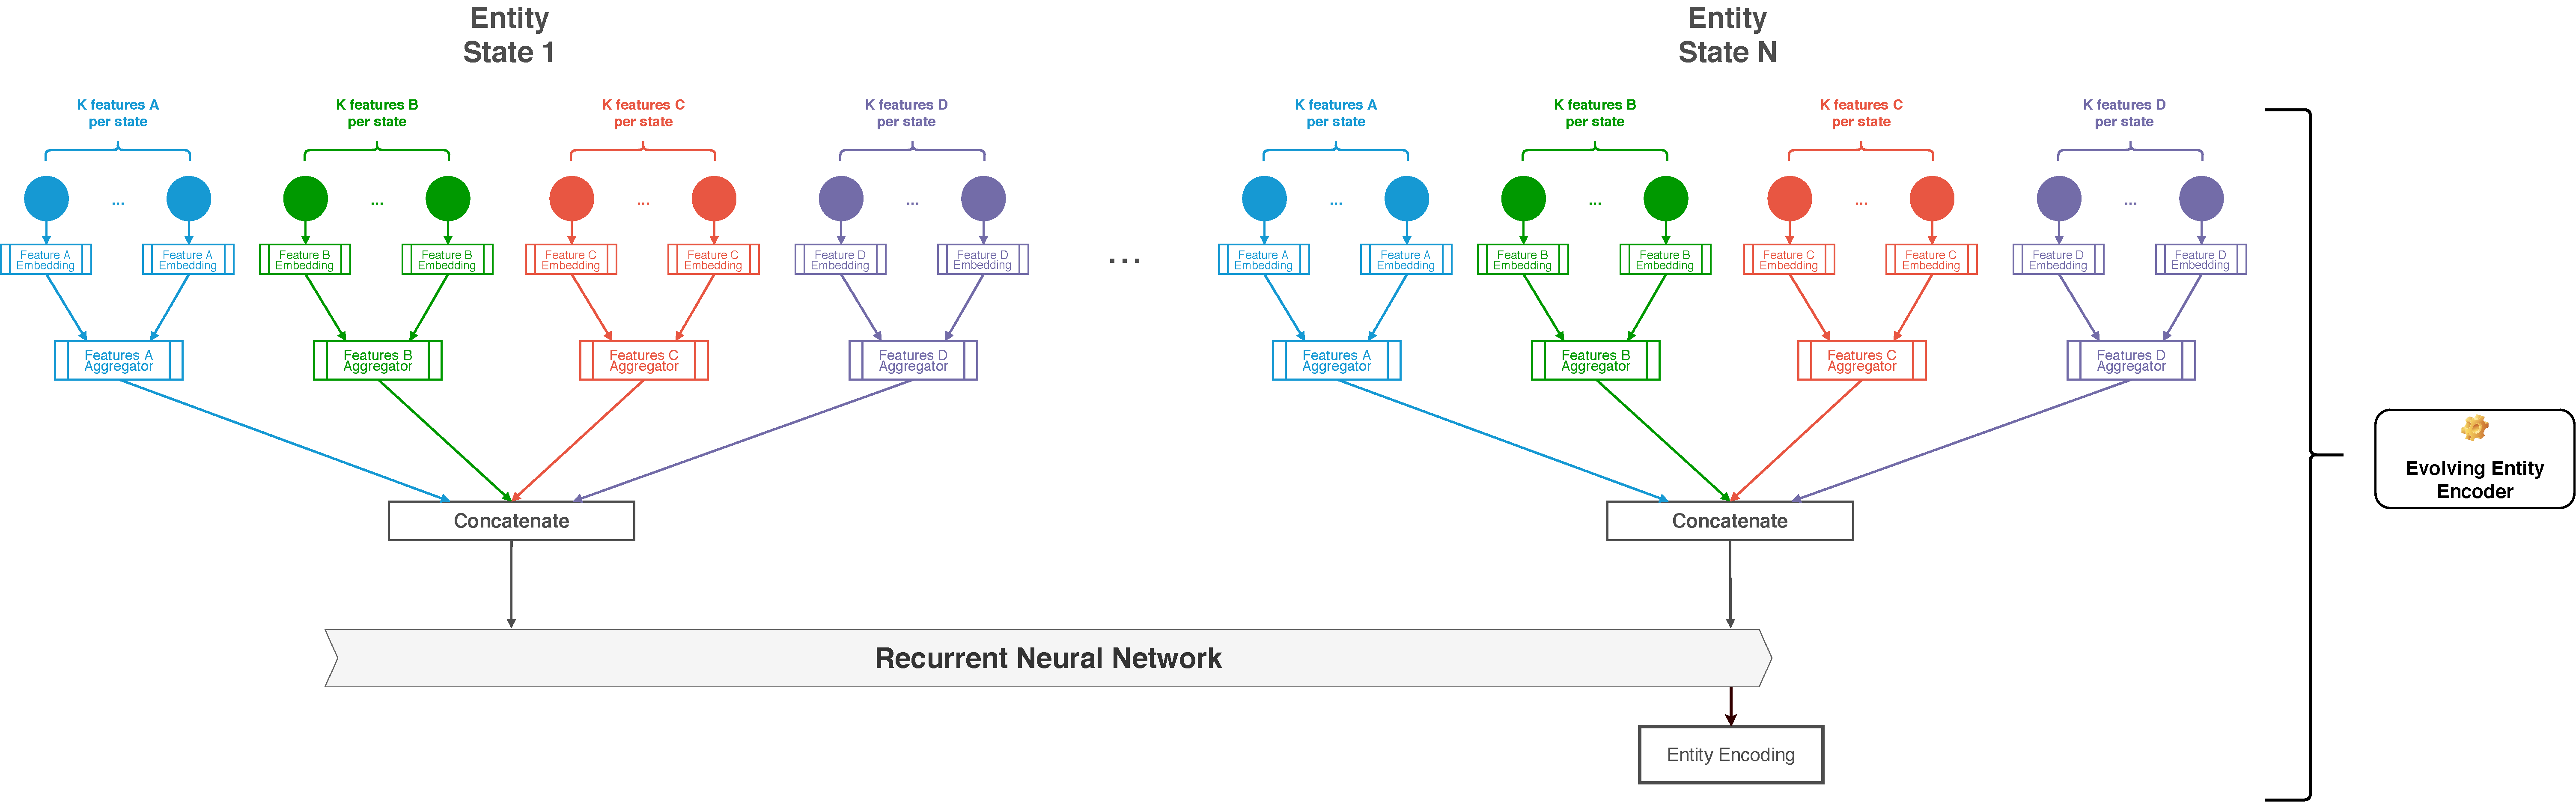
\includegraphics[width=\linewidth]{figures/encoder-general.pdf}
  
  \caption{Visualization of the \emph{Evolving Entity Encoder}, that passes each feature through their respective embedding, then aggregator and concatenate the results to be finally fed through the Recurrent Neural Network. This is application-agnostic and supports a varying number of features for each entity.}
 \end{figure}
\end{landscape}
\newpage
\begin{landscape}
\begin{figure}[H]
 \centering
 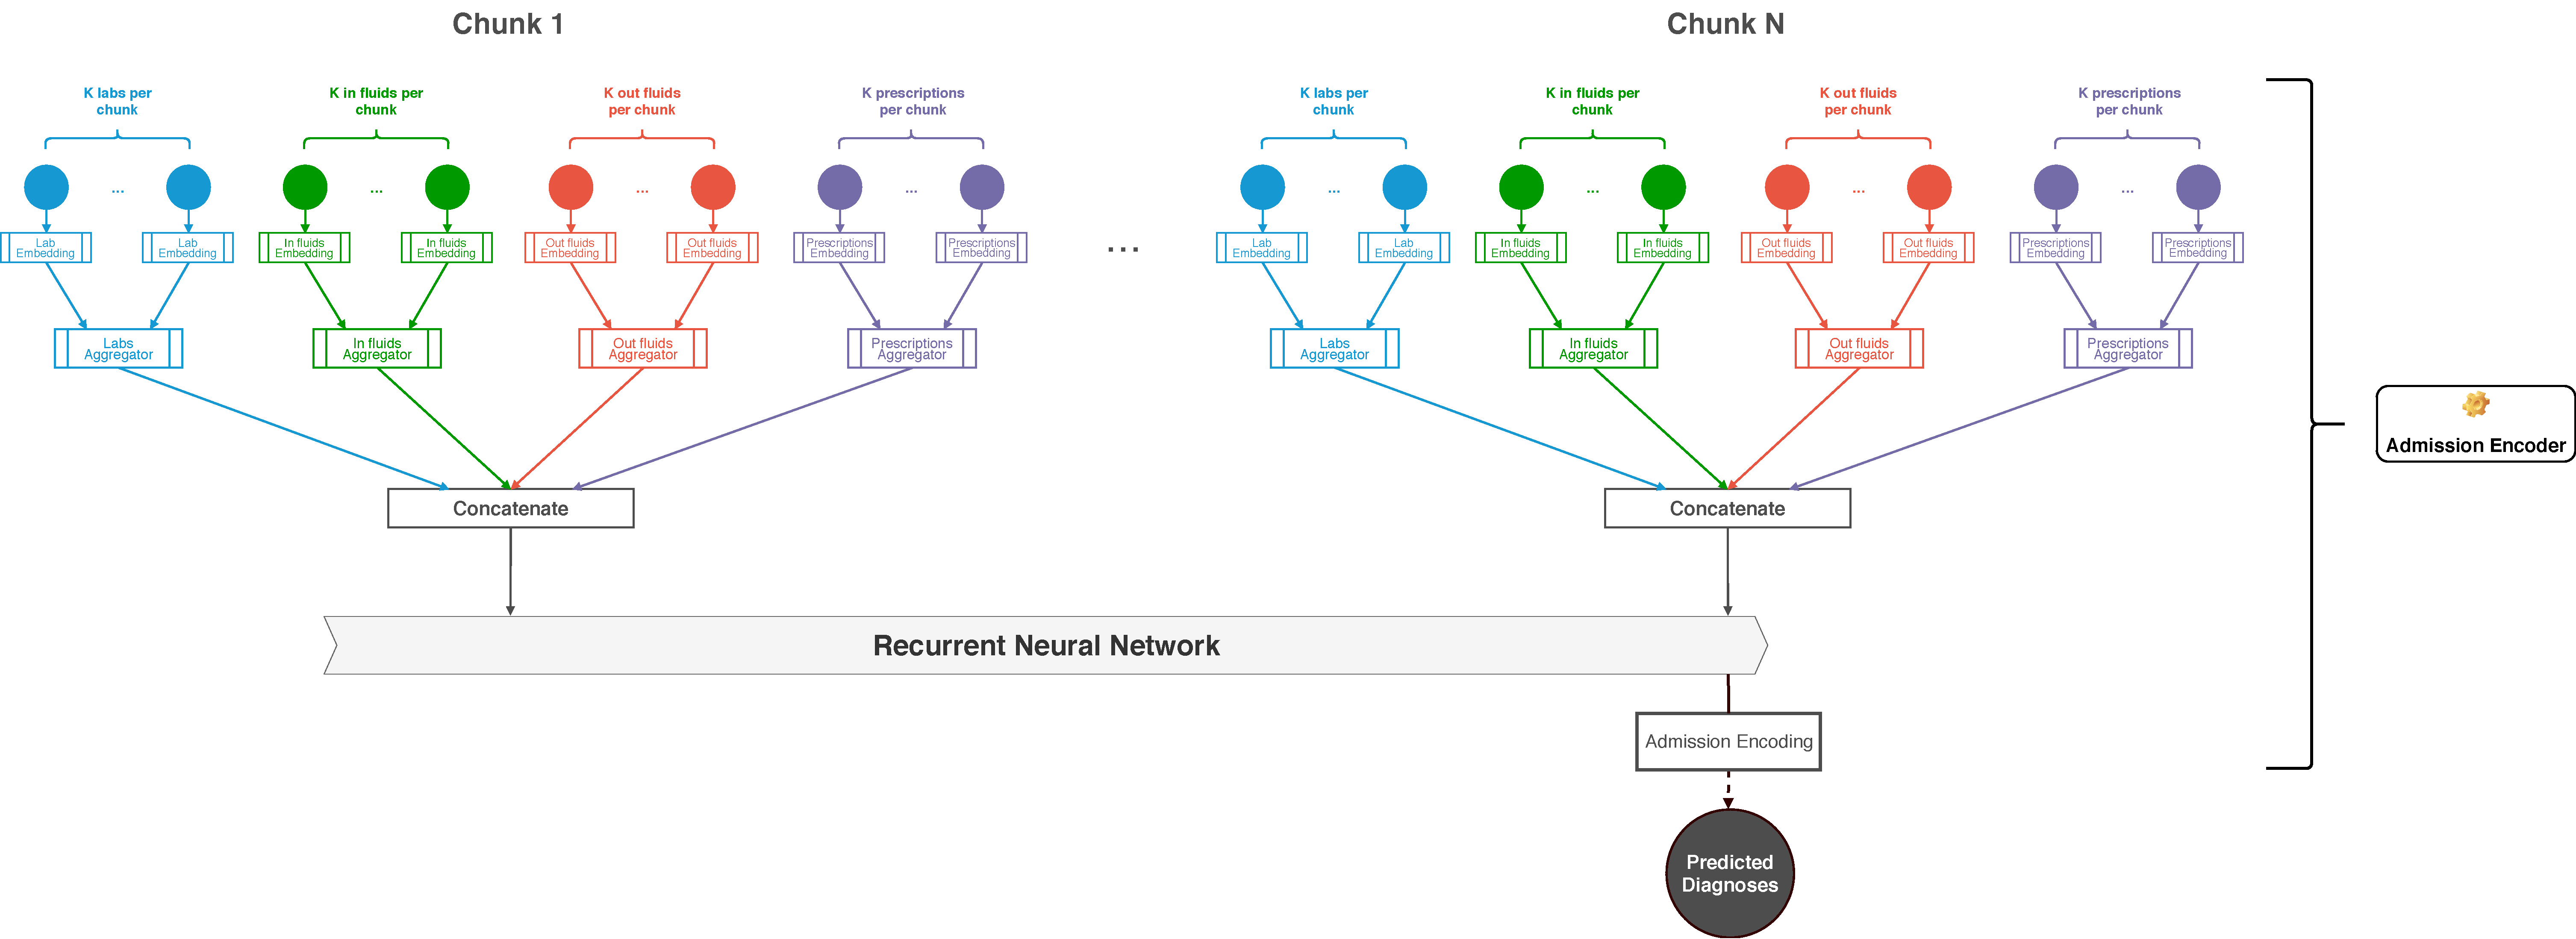
\includegraphics[width=\linewidth]{figures/encoder-healthcare.pdf}
 
 \caption{The \emph{Evolving Entity Encoder} applied to our use-case. Hence, we are encoding an admission that consists in an evolving patient state to finally predict the diagnoses at discharge with an additional fully-connected layer.}
\end{figure}
\end{landscape}
\chapter{KG-RNN: Our Architecture}
\label{chap:KG-RNN}
In this chapter we introduce our own architecture, based on the previous chapter where we present our \textbf{Evolving Entity Encoder}. This novel architecture leverage different graph theory techniques and machine learning to encompass information from other entities and thus further boost the predictive power of the model. \\

The first section will highlight the different steps of the pipeline, then the following section describes the process of constructing the weighted knowledge graph from internal (MIMIC-III) as well as external information. Right after, we develop the idea of ``extracting`` other entities of interest from the knowledge graph that will improve the prediction for a given input entity. Finally, we expose our \emph{KG-RNN} deep learning architecture to leverage the input entity as well as the ones we extracted in the previous stage.

\section{Overview}
Our ``KG-RNN`` architecture extends on the previous baseline described in chapter~\ref{chap:Baseline}. The novelty and improvement rely on neighboring entities of interest (i.e. admissions in our use-case) to encompass more information than solely the input entity. \\

To do so, the first phase consists in creating an appropriate knowledge graph from our dataset but also external information to enrich the linkage structure between entities. This can be done in many different ways, in a weighted or unweighted fashion ($w=1$), and we will describe here how we proceeded in the healthcare use-case. \\

Right after, from this enhanced knowledge graph, weighted or not, we have to extract neighboring entities of interest. For this purpose, we can employ any graph sampling technique (leveraging edge weight or not) and we will go through the one we chose. Finally, from the extracted neighbors and the input entity, we build a machine learning model extending from the baseline one to convey information from these neighbors.

\section{Weighted Knowledge Graph Construction}
As a first step and to the end of building our weighted knowledge graph, the main field of interest is~\emph{DIAGNOSIS} (that we will call ``prediagnosis`` hereafter to avoid confusion with ICD9 diagnoses) in the admission table. Firstly, we clean the prediagnosis: \begin{enumerate*}\item Converting to lower-case. \item Remove non-alphabetic characters. \item Remove multi-spaced as well as leading and trailing ones.\end{enumerate*} \\

On top of this \textit{prediagnosis}, we leverage external information from a recent paper that creates a mapping between diseases and symptoms~\cite{Rotmensch2017}. This external knowledge graph is built from Electronic Health Records (EHR) and links diseases with their respective symptoms, while providing a symptom relevance weight (between 0 and 1). An example of entry from this external source is: \emph{Migraine: Headache ($w=0.384$), nausea ($w=0.316$), sensitivity to light ($w=0.223$), ...} These diseases and symptoms are cleaned in the exact same way as the prediagnosis and assembled to create our \textbf{dictionary}. \\ 

Our goal now is to link the external information with our internal information to create an enriched knowledge graph. We want to link prediagnosis with symptoms and diseases, while these latter two are intrinsically linked directly by the external information (cf. \textit{Migrain} example above). \\

To this end we have to cope with the problem of spelling mistakes as well as quasi-similar prediagnosis and diseases/symptoms (e.g. ``Coronary heart disease`` vs. ``Arteries heart disease``), we create a character N-grams~\footnote{\url{https://en.wikipedia.org/wiki/N-gram}} (where the size of the n-gram has to be tuned) list from the cleaned entries of the dictionary (prediagnosis, disease and symptoms). From this n-grams list, we create a TF-IDF~\footnote{\href{https://en.wikipedia.org/wiki/Tf\%E2\%80\%93idf}{https://en.wikipedia.org/wiki/Tf\_idf}} vector with a minimum document frequency of 1. \\

Finally, we match prediagnosis with diseases and symptoms based on the cosine similarity between their n-grams + TF-IDF vectors. Namely, we link a prediagnosis with a disease and a symptom if their cosine similarity score is above a given threshold (to manually filter out noise), and we link diseases and symptoms based on the external information while also applying a threshold on the symptoms relevance weight provided out-of-the-box by the external source. The final knowledge graph is represented in the figure~\ref{fig:kg-healthcare}, including both internal and external information. \\

\begin{figure}[H]
 \centering
 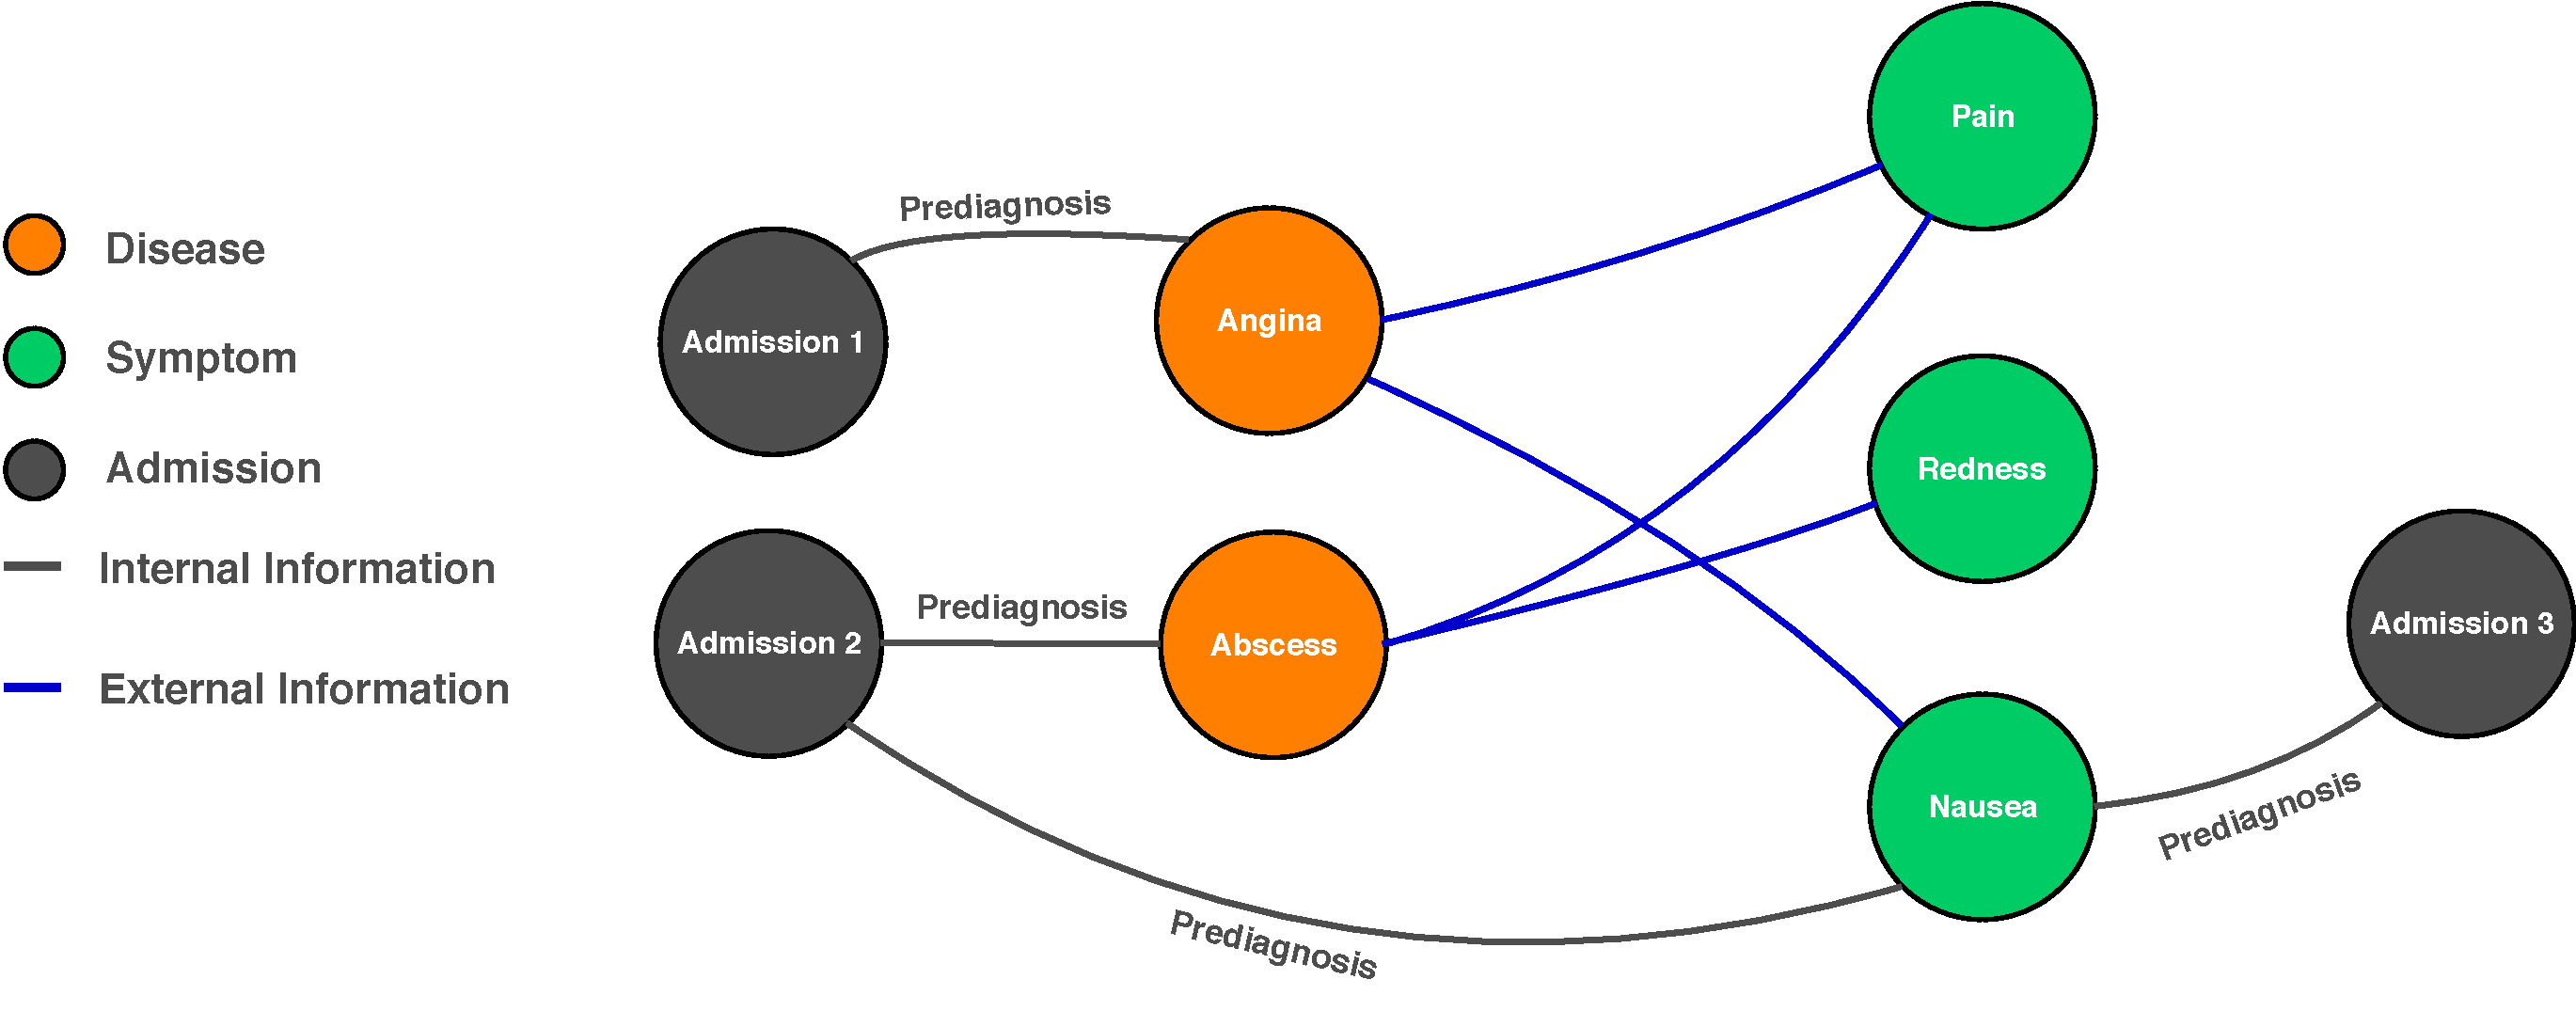
\includegraphics[width=0.9\textwidth]{figures/kg-healthcare.pdf}
 \caption{Final knowledge graph made of external and internal information that will be used in the experiments and discussions.}
 \label{fig:kg-healthcare}
\end{figure}

On a practical note, for the rest of the discussions and experiments, we set n-grams to \textbf{3 characters}, the minimum cosine similarity score of \textbf{0.6} and a relevance weight between diseases and symptoms of \textbf{0.2}.

\newpage
\section{Weighted Knowledge Graph Extraction}
Secondly, from this weighted knowledge graph, we want to extract relevant neighboring entities to enrich our input entity with additional information. For this purpose, one can use any graph sampling technique~\cite{DBLP:journals/corr/HuL13, Leskovec:2006:SLG:1150402.1150479}, making use of the weights defined during \textit{Graph Construction} or not. \\

This graph sampling will be very important for the downstream model and also the number of neighbors is a critical hyper-parameter that has to be tuned. In that regard, relevant experiments can be found in the appropriate chapter. Some common sampling techniques could be \begin{enumerate*}\item Random sampling on 1-hop neighbors. \item Snow-Ball sampling. \item Forest Fire sampling.\end{enumerate*}. \\

For our use-case at hand, we decided to employ some \textit{importance sampling} based algorithm. This technique is inspired from a paper~\cite{DBLP:journals/corr/abs-1806-01973} by Pinterest and Stanford, it relies on random walks to create an importance score for each entity and take the top scoring entities as neighbors of interest. \\

Concretely, the process is to simulate many random walks \emph{starting from input entity} and compute the $L_1$-normalized visit count as the importance score. Now, instead of simulating thousands of random walks it can be proven that in the limit of an infinity of simulations, the normalized $L_1$ visit count is equivalent to a Personalized PageRank score. Henceforth, we decided to compute the Weighted Personalized PageRank score (personalized on the input entity) using \textit{Oracle PGX} for each input entity. \\

Finally, and as stated previously, the top-$M$ scoring entities are extracted for each input admission and we define a minimum score of \textbf{0.0001} as an arbitrary threshold. Otherwise, there would always have exactly M neighbors sampled even if some are isolated and thus have a score of 0. This threshold allows for more flexibility and to have $0 \leq \mbox{neighbors} \leq M$ for a given input admission. \\

From a practical standpoint, we also make sure not to sample neighbors from the testing or validation set when we are training, or respectively sampling entities from the training or testing set during validation. Equivalently, we make sure not to sample entities from training and validation when we do the final evaluation on the test set.

\section{Graph Machine Learning}
The machine learning model encapsulating information from neighboring entities as well as the input entity relies on the building block described in the chapter~\ref{chap:Baseline}. Indeed, the input admission is first encoded using the \textbf{Evolving Entity Encoder} from which the final embedding vector $\bm{\tilde{h}} \in \mathbb{R}^{b}$ is fed to the main module. The main module job lies in blending information from extracted neighbors with the input admission vector $\bm{\tilde{h}}_i^m$. \\

To better understand the mechanics, the extracted neighbors can be seen as made of static information throughout admission (e.g. patient age) and dynamic information (e.g. their respective events). The main module can either process dynamic information and static information, or just one or the other. Explicitly, the extracted neighbors entities can also go through the Evolving Entity Encoder to embed their dynamic behavior in a vector $\bm{\tilde{h}} \in \mathbb{R}^{b}$ that will be then concatenated with static information vectors. \\

Eventually, the embedded vector is concatenated with static information vectors, and fed through a fully-connected layer (\textit{encoder}) to obtain the final neighbor encoding vector. These vectors are then fed through an aggregator of the same kind as the one described in chapter~\ref{chap:Baseline}, that is \textit{sum}, \textit{mean} or \textit{max}. hHe purpose of this aggregator is to squash the data along the $M$ dimension to squeeze out information from neighbors. The final prediction diagnoses are made from the concatenation of the aggregated neighbors and input entity encoding, that is finally fed into a fully-connected layer mapping to our \emph{50} classes. \\

On our use-case at hand, we decided to discard dynamic behavior of neighbors and solely take into account the final diagnoses of those as our static information. Additionally, for a one-hot encoded vector of a neighbor final diagnoses $\bm{y}=[0, 0, 1, 0, 1, 0, \dots, 1]\mbox{, where }|\bm{y}|=50$ we decided to make use of the \textbf{SEQ\_NUM} field by transforming this one-hot vector using the function $1/x$. That is, our new static information vector becomes $\bm{\tilde{y}}=[0, 0, 1/1, 0, 1/3, 0, \dots, 1/2]\mbox{, where }|\bm{\tilde{y}}|=50$ if we respectively have a \textbf{SEQ\_NUM} of 1, 3 and then 2. \\

A schematic visualization of the general machine learning model is available on the figure~\ref{fig:kg-rnn-general}, while the applied model can be found on the figure~\ref{fig:kg-rnn-healthcare}.

\newpage
\subsection{Schematic Visualizations}
In order to provide the reader an overview of the mechanics behind KG-RNN, the following visualization summarizes the textual description of the previous section.

\begin{figure}[H]
 \centering
 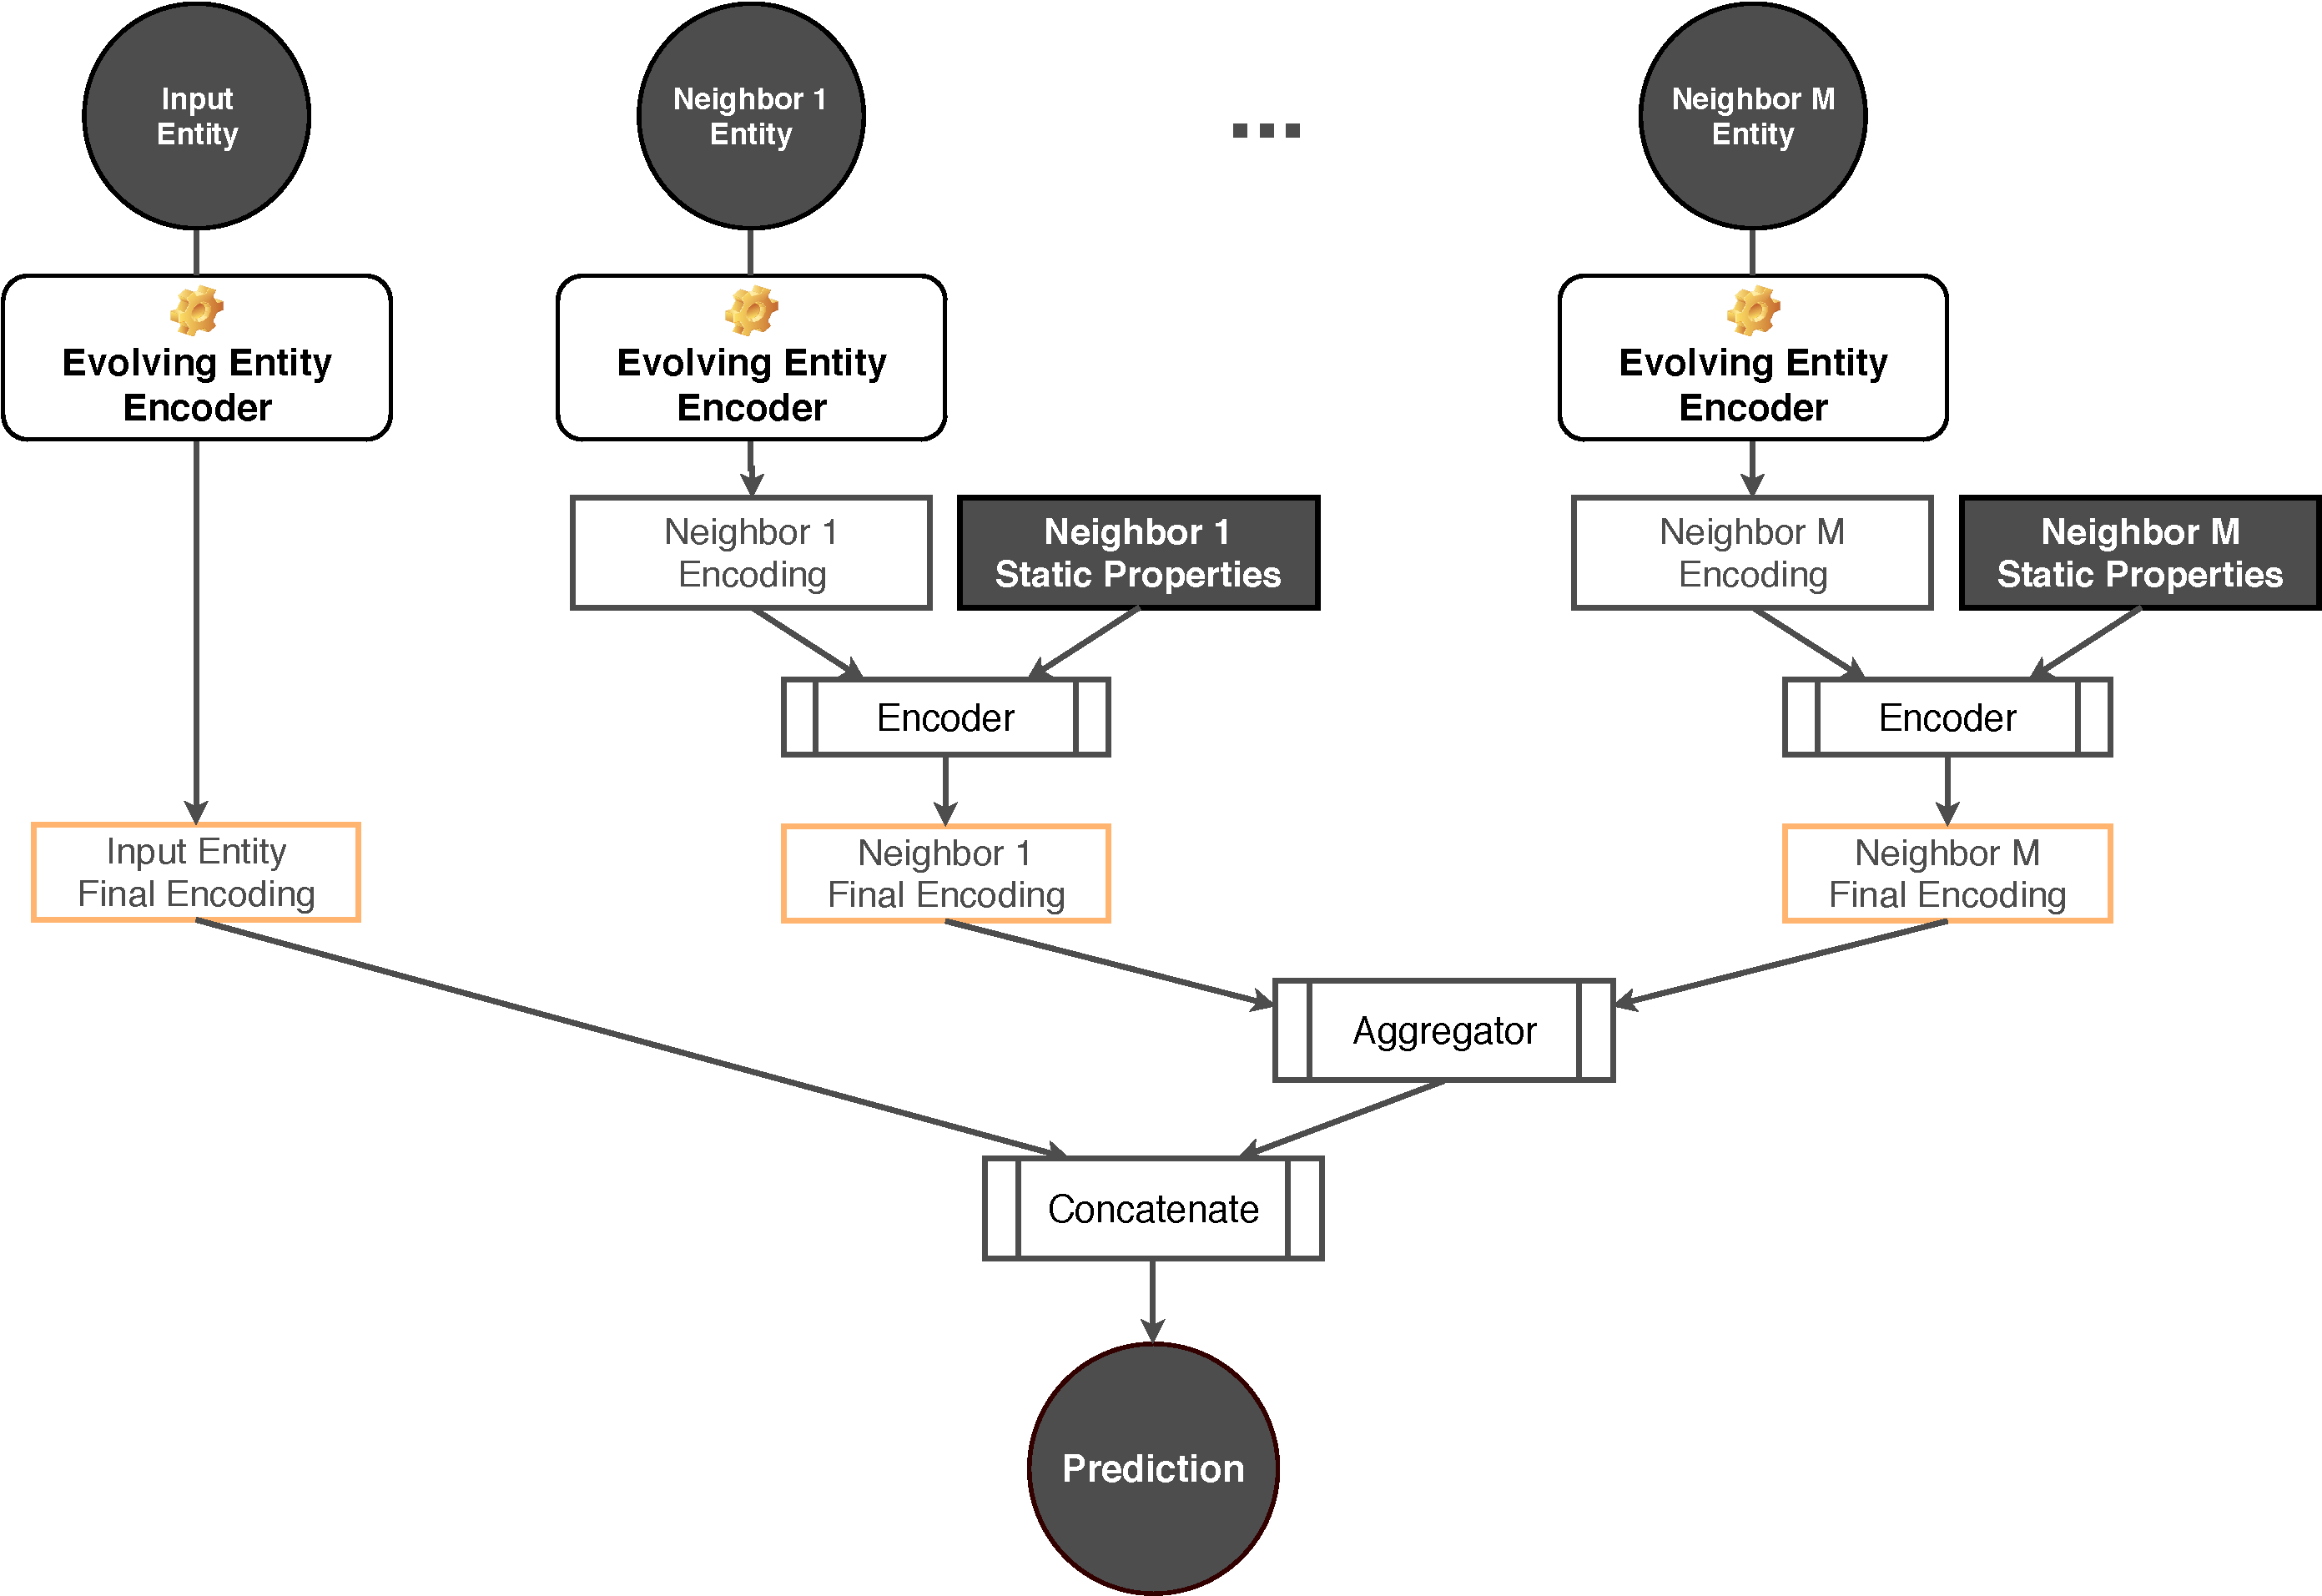
\includegraphics[width=0.7\textwidth]{figures/kg-rnn-general.pdf}
 \caption{The general module of our architecture, where \textbf{Evolving Entity Encoder} relies on work from previous chapter. The static properties and information from neighbors are concatenated and fed through an \emph{Encoder}, consisting of a simple fully-connected layers to blend the concatenated information. All encoding vectors from neighbors are aggregated along the $M$ dimension and concatenated with the input entity. This vector is then further fed into a fully-connected layer, here hidden in the \emph{Concatenate} block, to output the predictions.}
 \label{fig:kg-rnn-general}
\end{figure}

The following figure is a special case of the general approach available in the previous figure. Indeed, in our practical application we decided to get rid of the dynamic information from neighbors, leading to the following adapted schema:

\begin{figure}[H]
 \centering
 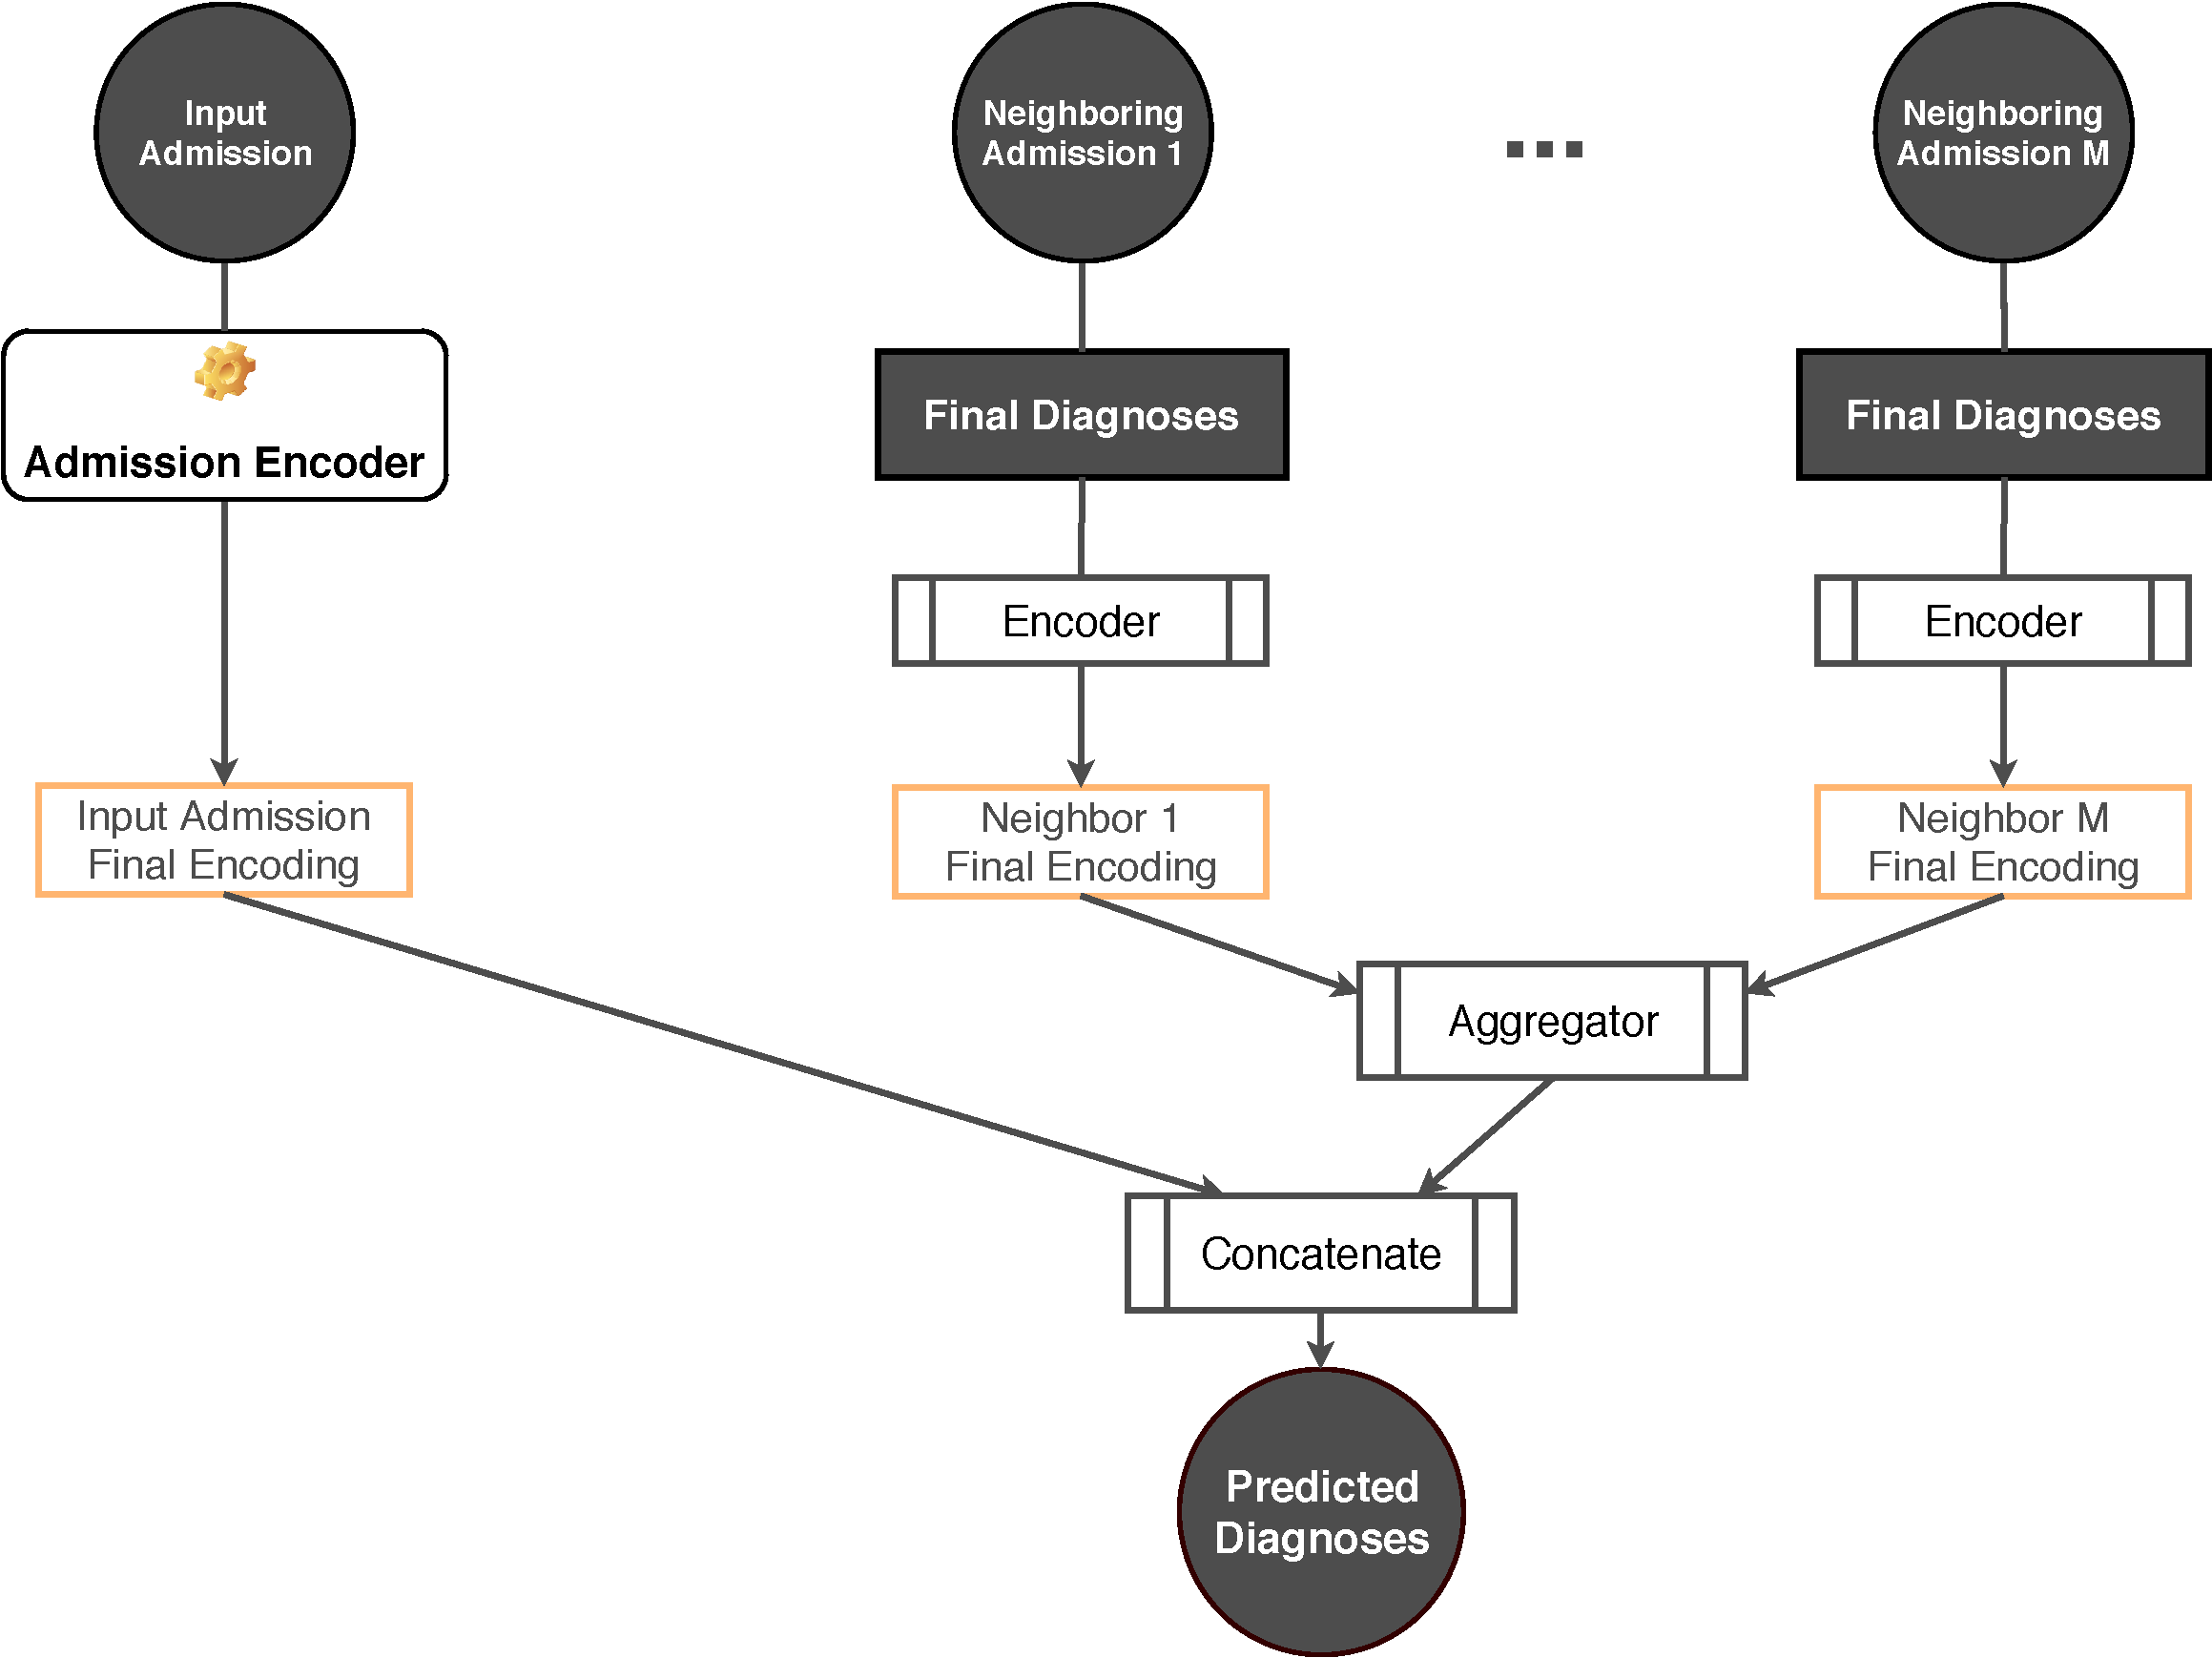
\includegraphics[width=0.6\textwidth]{figures/kg-rnn-healthcare.pdf}
 \caption{Similar to the previous schema, except that only static information from neighbors is encoded and squashed. Here the static information consist of only the diagnoses of these neighboring admissions.}
 \label{fig:kg-rnn-healthcare}
\end{figure}

As mentioned previously, in our case we decided to discard dynamic information from neighbors but we argue that this is heavily application-dependent, thus validating on different tasks and knowledge graphs would be insightful.
\chapter{Experiments}
\label{chap:Experiments}
This chapter describes the different experiments we ran as well as their respective results. It is heavily focusing on the task at hand, which is to \emph{predict the diagnosed top 50 most frequent ICD9 codes at discharge in a multi-class multi-classification fashion}. \\

The first section describes the setup in which the experiments are run, the optimizer as well as the hardware setting. Following to this, we get to the core of the chapter and explain our experiments we ran while providing the quantitative results on different metrics. Finally, from these experiments we conclude the chapter with a hyper-parameter tuning section detailing how we picked the deep learning hyper-parameters.

\section{Setup}
\label{sec:Setup}
All the experiments and training sessions were run on two \textbf{Tesla P100} with 16 GB of memory. The CPU was an \textbf{Intel Xeon Gold 5120 CPU @ 2.20 GHz}, with \textbf{56 cores}, while we had access to \textbf{187 GB of RAM} on the machine. On top of that, the different scripts and models have been built on \textit{Python 3.6.7} and we used \textit{Pytorch 1.0.0} as our Deep Learning framework. \\

We  employ  mini-batch  stochastic gradient descent method together with the Adam optimizer~\cite{DBLP:journals/corr/KingmaB14} to  minimize  our multi-class multi-classification loss. \\

To facilitate reading and understanding, we break down the different hyper-parameters in three groups:

\begin{itemize}
 \item Knowledge Graph
 \begin{itemize}
  \item $M$: number of neighbors
  \item Characters n-grams
  \item Weighted Personalized PageRank threshold
  \item Disease - Symptom threshold
  \item Admission - Symptom threshold
  \item Admission - Disease threshold
 \end{itemize}
 \item Admission Processing
 \begin{itemize}
  \item $N$: number of chunks
  \item $K$: number of events per chunk
  \item $\tau$: chunk length
 \end{itemize}
 \item Deep Learning
 \begin{itemize}
  \item $n$: events embedding dimension (potentially different for each event type)
  \item $a$: aggregators hidden dimension (for both input entity and neighbors, potentially different for each event type)
  \item Input entity aggregator type (max, mean or sum, potentially different for each event type)
  \item Neighbor entities aggregator type (max, mean or sum)
  \item RNN: number of layers
  \item RNN: number of neurons per layer
  \item RNN: dropout between layers
  \item RNN: bidirectional or not
  \item $b$: Recurrent Neural Network output dimension
  \item Batch size
 \end{itemize}
\end{itemize}

To reduce the search space, we contrived our hyper-parameters by fixing the same embedding dimension and aggregator for all events. Finally, we also decided to tune the \emph{Knowledge Graph} and \emph{Admission Processing} hyper-parameters while tuning the \emph{Deep Learning} ones. Consequently, we also did the opposite when tuning the \emph{Knowledge Graph} and \emph{Admission Processing} hyper-parameters. \\

This way, we limit the computation time while getting a pretty good idea of the top-performing configurations and interactions between theses hyper-parameters. We suppose that scores reported for the final task on the testing set could be further improved by fine-tuning all these hyper-parameters together instead of group-by-group. \\

Finally, we decided to split the \emph{58'976} in two groups, training and testing set, using an 80\%-20\% split. We then further holdout 10\% of this training set for validation purposes (the training set is thus 72\% of the total admissions while validation represents 8\% of these). \\

As a training strategy, we monitor different metrics, as explained in the section~\ref{sec:Metrics}, at each epoch and employ an early-stopping criterion on the validation loss with a patience of 20 epochs. That is, if the validation loss does not decrease within 20 epochs, the model is saved at its best scoring epoch and the training is considered finished.

\newpage
\section{Metrics}
\label{sec:Metrics}
\paragraph{F1 Score} The $F_1$ score is a particular case of the $F_\beta$ score which blends the well-known precision and recall scores. The $F_\beta$ score is computed as follows:

\begin{equation}
 F_\beta = (1+\beta)^2 \cdot \frac{\mbox{Precision} \cdot \mbox{Recall}}{(\beta^2 \cdot \mbox{Precision}) + \mbox{Recall}}
\end{equation}

Basically, the $\beta$ parameters dictate the importance we want to give to the precision or recall. By setting $\beta=1$, we give equal importance to both of them and above formula is equivalent to computing harmonic mean between the precision and recall. Our choice of $\beta=1$ is common and usually a good trade-off when there is no obvious preference between precision and recall.

\paragraph{Area Under Receiver Operating Characteristic} Often abbreviated \textit{AUROC}, this metric is coming from the receiver operating characteristic curve that is computed using the ``True positive rate`` and ``False positive rate``. This curve is particularly interesting since it reports the ability of our classifier to discriminate between positive and negative samples when the threshold varies. \\

Generally speaking, computing the area under this ROC curve is equivalent to the probability that a classifier will rank a positive random sample \textbf{higher} than a random negative one.

\paragraph{Macro and Micro Averages} To account for the slight class imbalance depicted in the top-right figure~\ref{fig:icd9-codes}, we consider two kinds of averages over classes scores, namely \emph{macro} and \emph{micro} averages. \\

The macro average will compute the metric independently for each class and then average globally, thus treating our different ICD9 codes equally. On the other hand, the micro average will first aggregate the contributions of all classes in order to compute the average metric. \\

We decided to compute both averages for our two metrics, leading to four combinations that we report in the experiments in sections~\ref{sec:Experiments}:

\begin{itemize}
 \item Macro-F1 Score
 \item Micro-F1 Score
 \item Macro-AUROC
 \item Micro-AUROC
\end{itemize}

\newpage
\section{Deep Learning Hyper-parameter Tuning}
For the hyper-parameter tuning of deep learning parameters, we fixed the \emph{Knowledge Graph} and \emph{Admission Processing} hyper-parameters to the following values:

\begin{itemize}
 \item Knowledge Graph
 \begin{itemize}
  \item $M=10$
  \item Characters n-grams = 3 characters
  \item Weighted Personalized PageRank threshold = 0.0001
  \item Disease - Symptom threshold = 0.2
  \item Admission - Symptom threshold = 0.6
  \item Admission - Disease threshold = 0.6
 \end{itemize}
 \item Admission Processing
 \begin{itemize}
  \item $N = 200$
  \item $K = 25$
  \item $\tau = 3 \mbox{ hours}$
 \end{itemize}
\end{itemize}
\subsection{Method}

All the scores were computed on the validation set, leaving the testing one untainted to prevent overfitting. The best scoring model was chosen accordingly and in accordance to performances on the validation loss. \\

We employed a very simple \emph{random search} as a sampling strategy of the next set of hyper-parameters during the optimization. This allows for much better results than a typical grid search that has the tendency to explore only a small subset of the search space. This strategy is also proven to show very good performances when the number of \textit{trials} is limited ($\leq 100$ in our case) for a very large search space, on top of the ease of implementation compared to more advanced sampling strategies.

\subsection{Search space}
The search space in our case consisted of:

\begin{itemize}
 \item $n \in \{8, 16, 32, 64, 128\}$, same for all event types
 \item $a=64$, same for input entity, neighbors and all event types
 \item $\mbox{agg}_{\mbox{input}} \in \{\mbox{max}, \mbox{mean}, \mbox{sum}\}$, same for all event types
 \item $\mbox{agg}_{\mbox{neighbors}} \in \{\mbox{max}, \mbox{mean}, \mbox{sum}\}$, same for all event types
 \item $\mbox{RNN}_{\mbox{layers}} \in \{1, 2, 3, 4, 5\}$
 \item $\mbox{RNN}_{\mbox{neurons}} \in \{64, 128, 256, 512\}$
 \item $\mbox{RNN}_{\mbox{dropout}} \in \{0, 0.1, 0.25, 0.5\}$
 \item $\mbox{RNN}_{\mbox{bidirectional}} \in \{\mbox{True}, \mbox{False}\}$
 \item $\mbox{RNN}_{\mbox{output size}} = 64$
 \item $\mbox{Batch size} \in \{4, 8, 16, 32, 64, 128\}$
\end{itemize}
Which leaves us with a search space of $5 \times 3 \times 3 \times 5 \times 4 \times 4 \times 2 \times 6 = 43'200$ possibilities.

\subsection{Results}
\paragraph{Baseline} We obtained the following best-scoring combination of hyper-parameters for the baseline:
\begin{itemize}
 \item $n = 64$
 \item $a = 64$
 \item $\mbox{agg}_{\mbox{input}} = \mbox{mean}$
 \item $\mbox{RNN}_{\mbox{layers}} = 1$
 \item $\mbox{RNN}_{\mbox{neurons}} = 128$
 \item $\mbox{RNN}_{\mbox{dropout}} = 0.25$
 \item $\mbox{RNN}_{\mbox{bidirectional}} = \mbox{True}$
 \item $\mbox{RNN}_{\mbox{output size}} = 64$
 \item $\mbox{Batch size} = 16$
\end{itemize}
Which translates to a particularly lightweight model, indicating the tendency of the baseline to overfit rather quickly.
\paragraph{KG-RNN} We obtained the following best-scoring combination of hyper-parameters for the baseline:
\begin{itemize}
 \item $n = 16$
 \item $a = 64$
 \item $\mbox{agg}_{\mbox{input}} = \mbox{max}$
 \item $\mbox{agg}_{\mbox{neighbors}} = \mbox{mean}$
 \item $\mbox{RNN}_{\mbox{layers}} = 2$
 \item $\mbox{RNN}_{\mbox{neurons}} = 128$
 \item $\mbox{RNN}_{\mbox{dropout}} = 0.5$
 \item $\mbox{RNN}_{\mbox{bidirectional}} = \mbox{False}$
 \item $\mbox{RNN}_{\mbox{output size}} = 64$
 \item $\mbox{Batch size} = 128$
\end{itemize}
It is important to notice that this top-scoring configuration consists in using a different kind of aggregator for neighboring admissions and input events. \\

One could argue that using a \emph{max-pooling} for input events and \emph{mean-pooling} for neighbors final diagnoses make sense since we can hypothesis that most salient events are important for a single patient, while blending the final diagnoses of neighbors allows to account for their relative contributions. \\

\section{Experiments}
\label{sec:Experiments}
Each experiment is broken down in a short description of the experiment and the associated results and graphics, followed by a ``discussion`` section where we interpret the results and plots. \\

All of these are on validation set for sake of keeping the testing set untainted until the final evaluation of the task at hand, namely ICD9 code prediction. Therefore, results of the different metrics, presented in sections~\ref{sec:Metrics}, are computed on the validation set for all experiments and compared to the baseline scores on each figure. \\

For all these experiments, the base setup of hyper-parameters are the one from the previous section for the \emph{Deep Learning} group. For the two other groups, here are the default parameters we chose:

\begin{itemize}
 \item Knowledge Graph
 \begin{itemize}
  \item $M=10$
  \item Characters n-grams = 3 characters
  \item Weighted Personalized PageRank threshold = 0.0001
  \item Disease - Symptom threshold = 0.2
  \item Admission - Symptom threshold = 0.6
  \item Admission - Disease threshold = 0.6
 \end{itemize}
 \item Admission Processing
 \begin{itemize}
  \item $N = 200$
  \item $K = 25$
  \item $\tau = 3 \mbox{ hours}$
 \end{itemize}
\end{itemize}

These are the hyper-parameters to be assumed except for the varying one in each experiment, that will be reminded in the relevant subsection. It is important to bear in mind that complex interactions within hyper-parameters are not taken into account in these experiments since we tune one degree of freedom at a time. \\

It would be very interesting to run these experiments with more computational power and time to account for much more precise hyper-parameter tuning and visualize how the metrics react for possibly more complex combinations.

\newpage
\subsection{Chunk length}
In this experiment we make the number of hours per chunk vary. This means that we consider the larger time window as the current graph state. Thus, it should have an impact on the amount of information fed to \emph{KG-RNN}, especially its aggregators.

\begin{figure}[H]
 \centering
 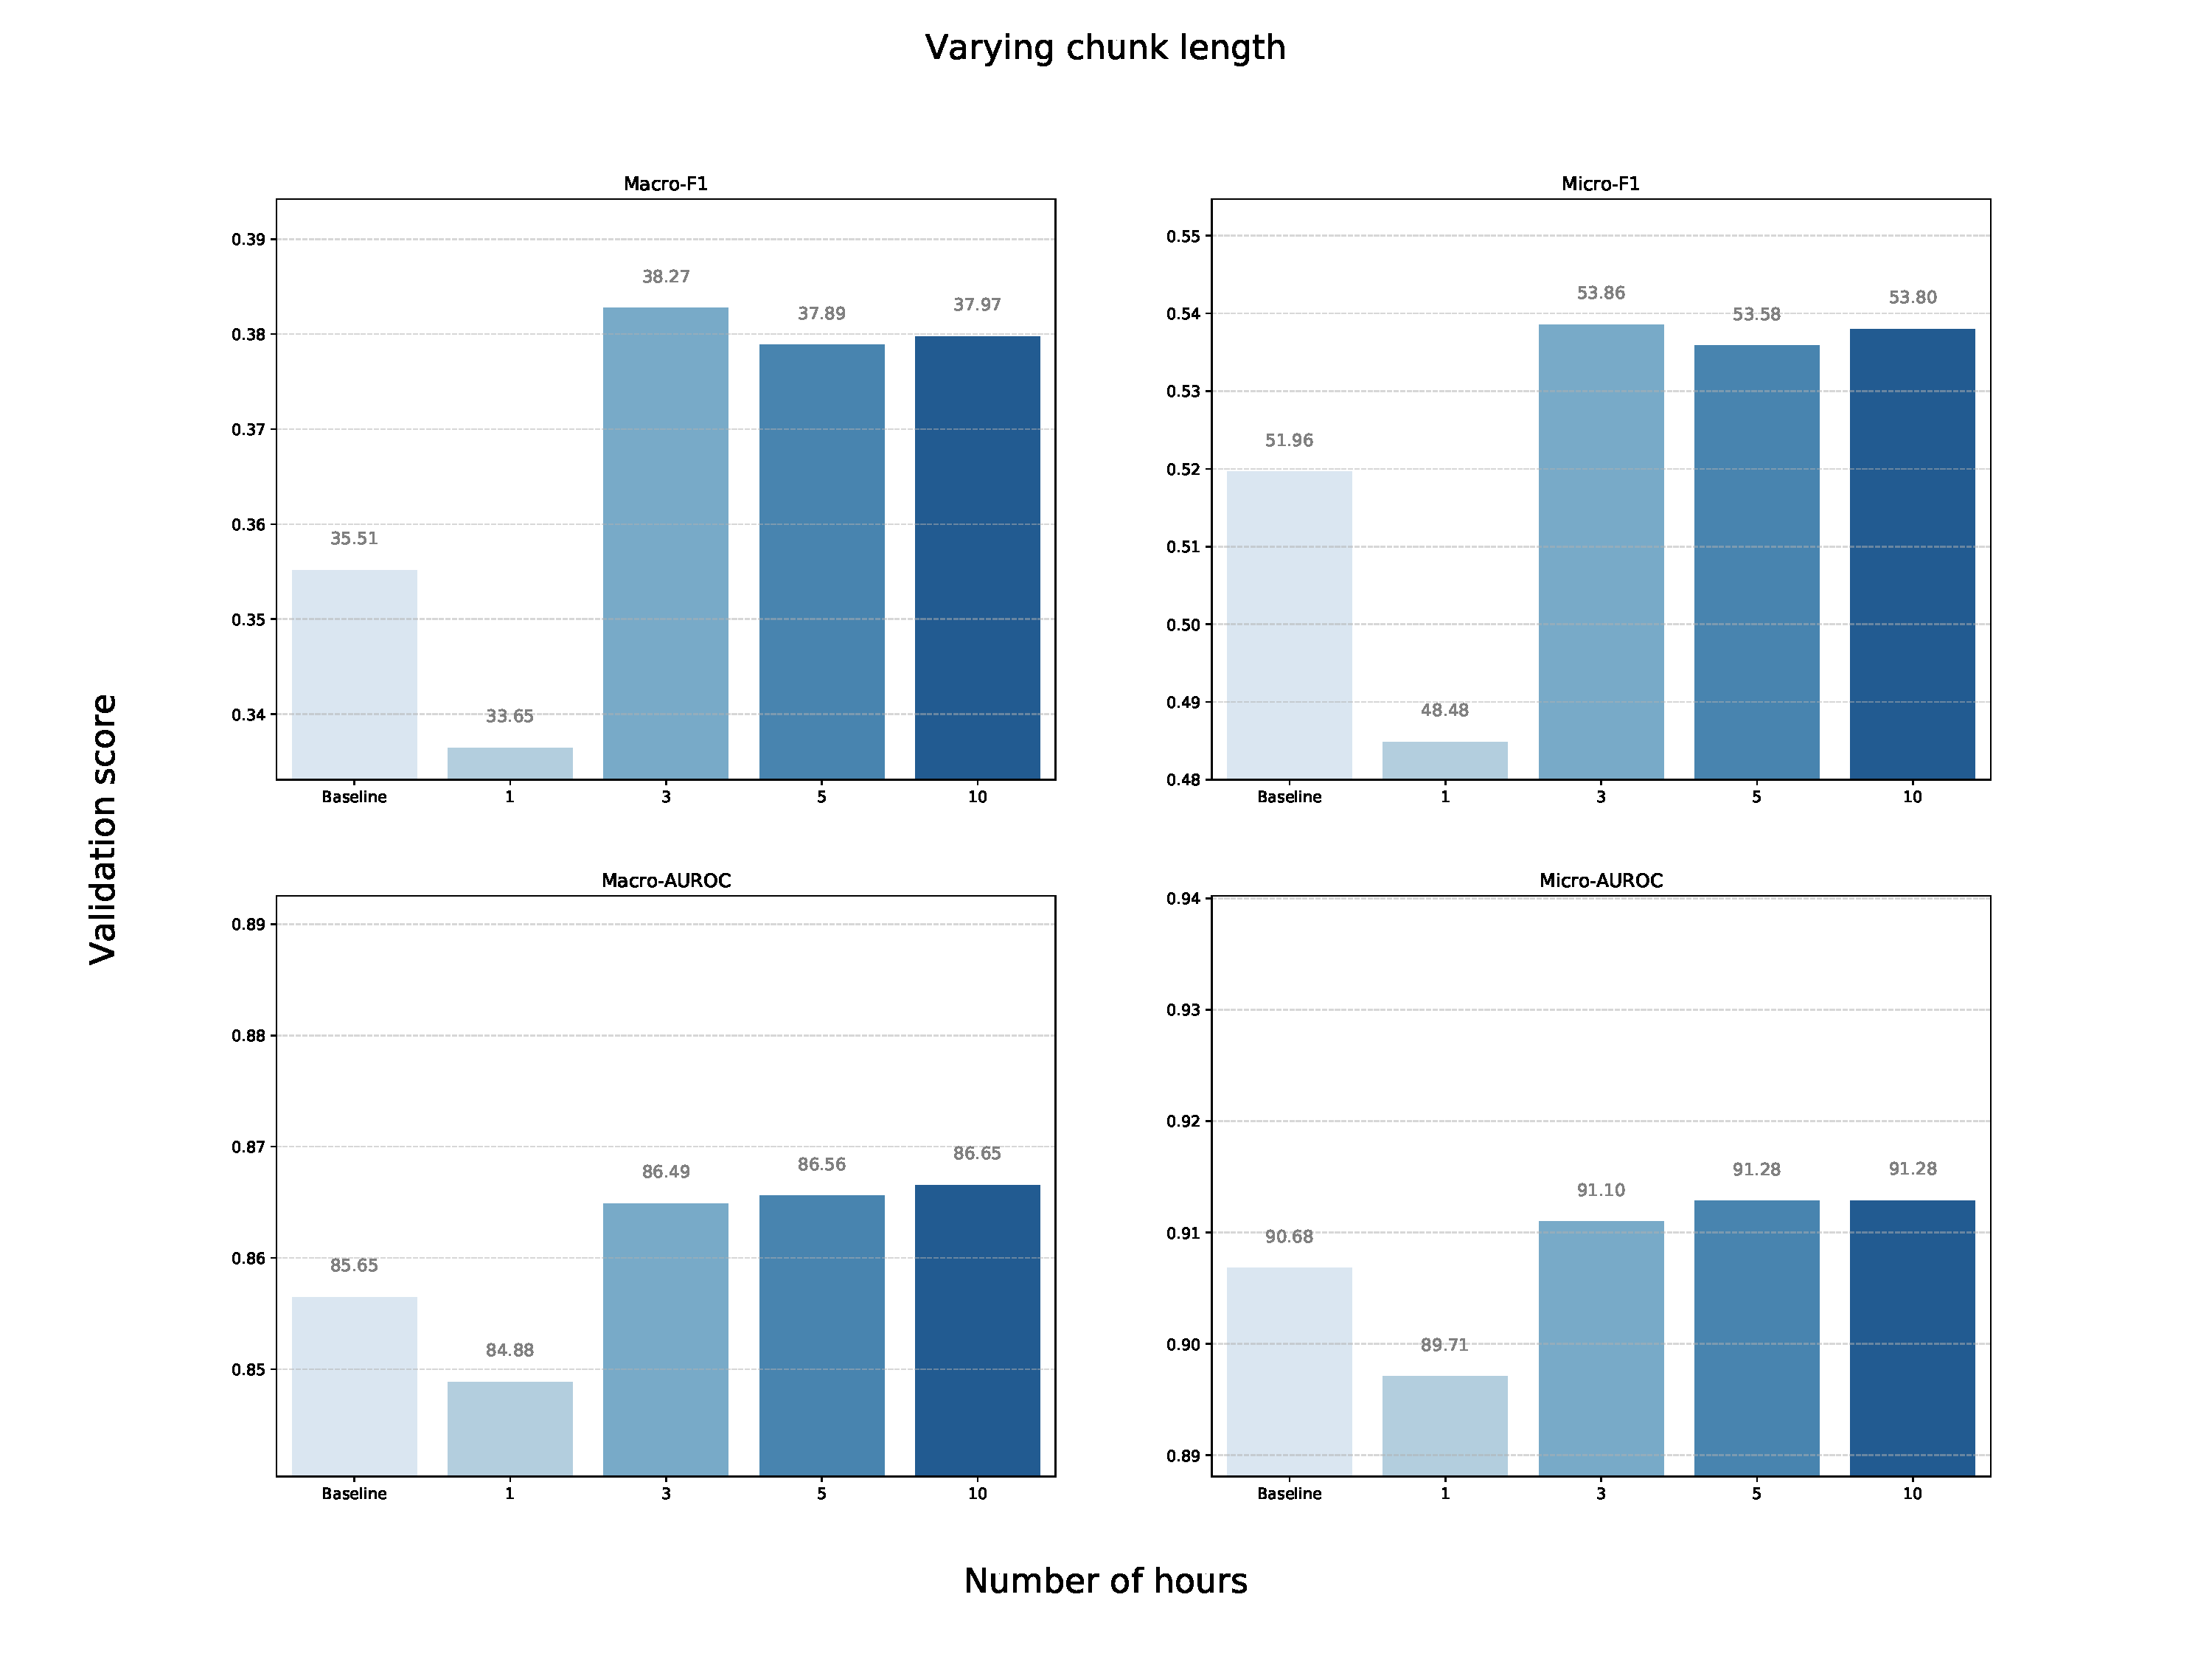
\includegraphics[width=\textwidth]{figures/exp-hours.pdf}
\end{figure}

\paragraph{Discussion} We see that the number of hours per chunk does not have a huge impact after 3 hours. However, setting the chunk length to small (i.e. 1 hour) makes the graph state probably too sparse in terms of the number of events.

\newpage
\subsection{Admission length}
This experiment makes the number of chunks per admission vary, also referred as the number of graph states. This will have the impact of increasing the size of sequences that are fed to the downstream Recurrent Neural Network and challenge its capacity to encode long-term dependencies in the input sequences.

\begin{figure}[H]
 \centering
 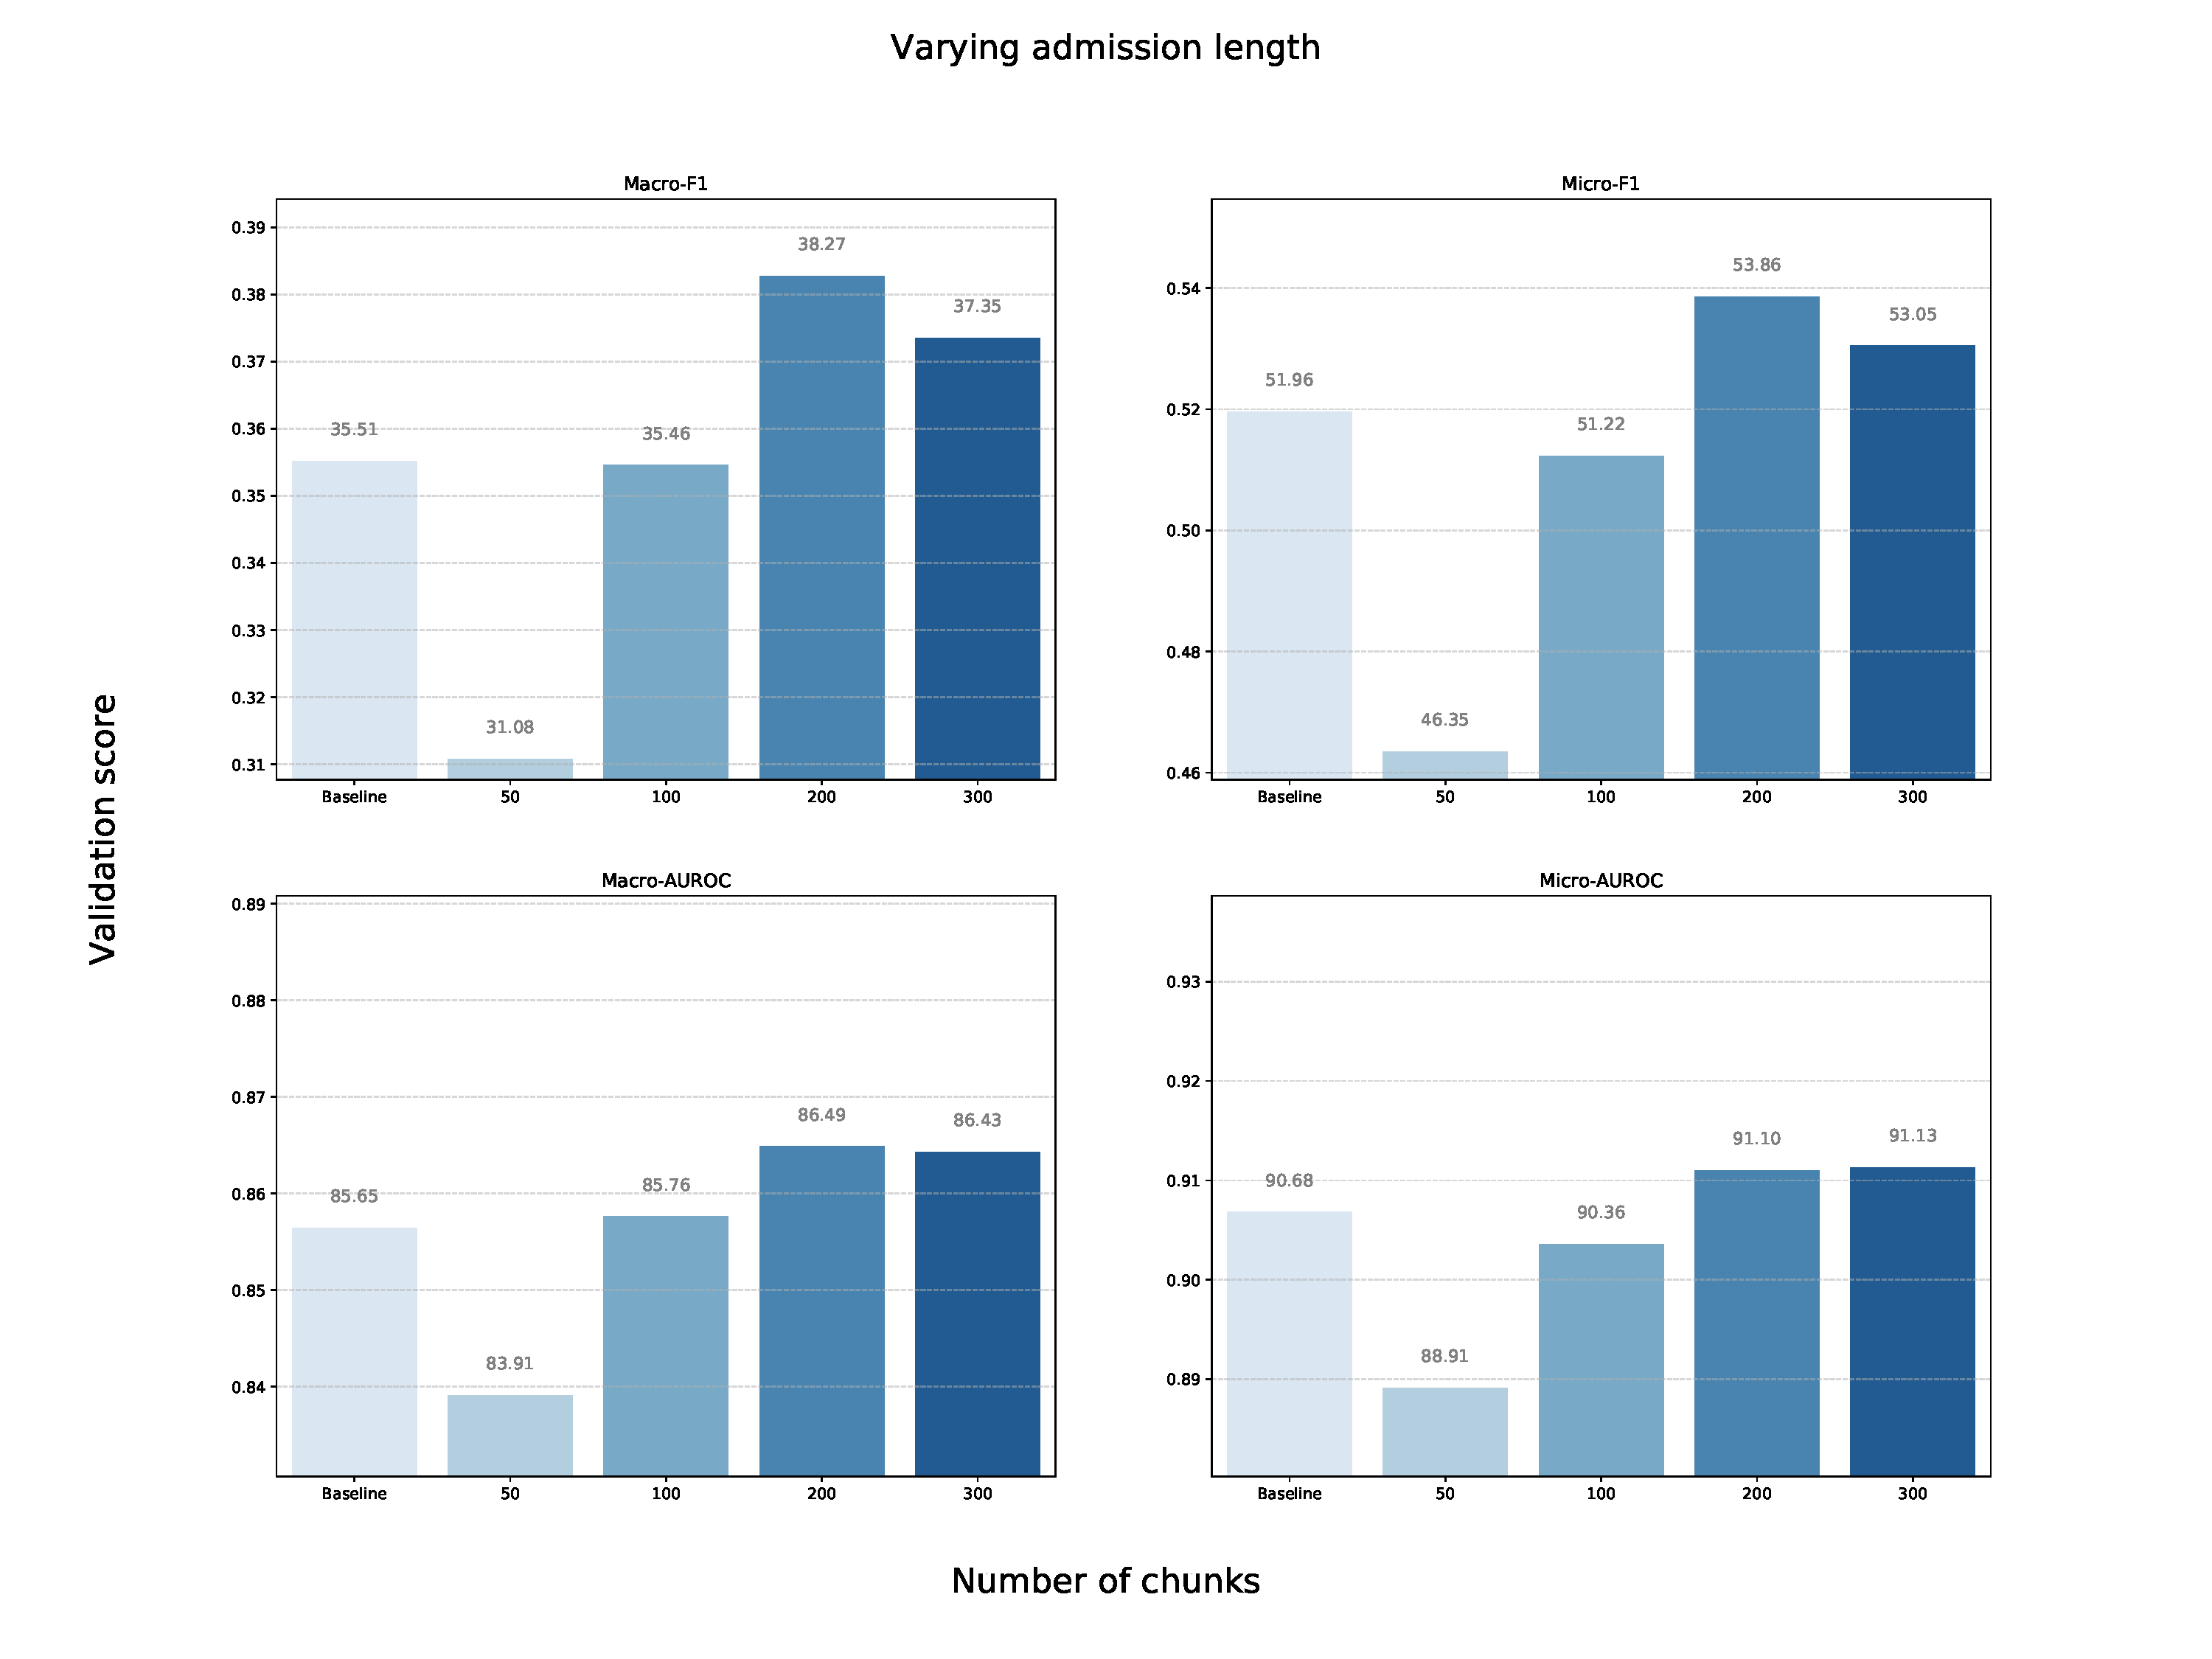
\includegraphics[width=\textwidth]{figures/exp-chunks.pdf}
\end{figure}

\paragraph{Discussion} In the above figure, we clearly see that we obtain a local optimum with an admission length of \emph{200} for the F1 score. However, the optimal value for the AUROC score is not so clear cut and further investigation would be beneficial in terms of interaction with the \textbf{chunk length}. \\

Indeed, since the total considered time for an admission is $\mbox{chunk length} \times \mbox{admission length}$, both parameters are intrinsically linked and probably heavily correlated.

\newpage
\subsection{Number of events per chunk}
For this experiment, we vary the \textit{maximum} number of events per chunk and per type. Chunks that have more than this number of events in a chunk for a given type will be randomly sampled to $K$, while other ones remain with their number of events $\leq K$.

\begin{figure}[H]
 \centering
 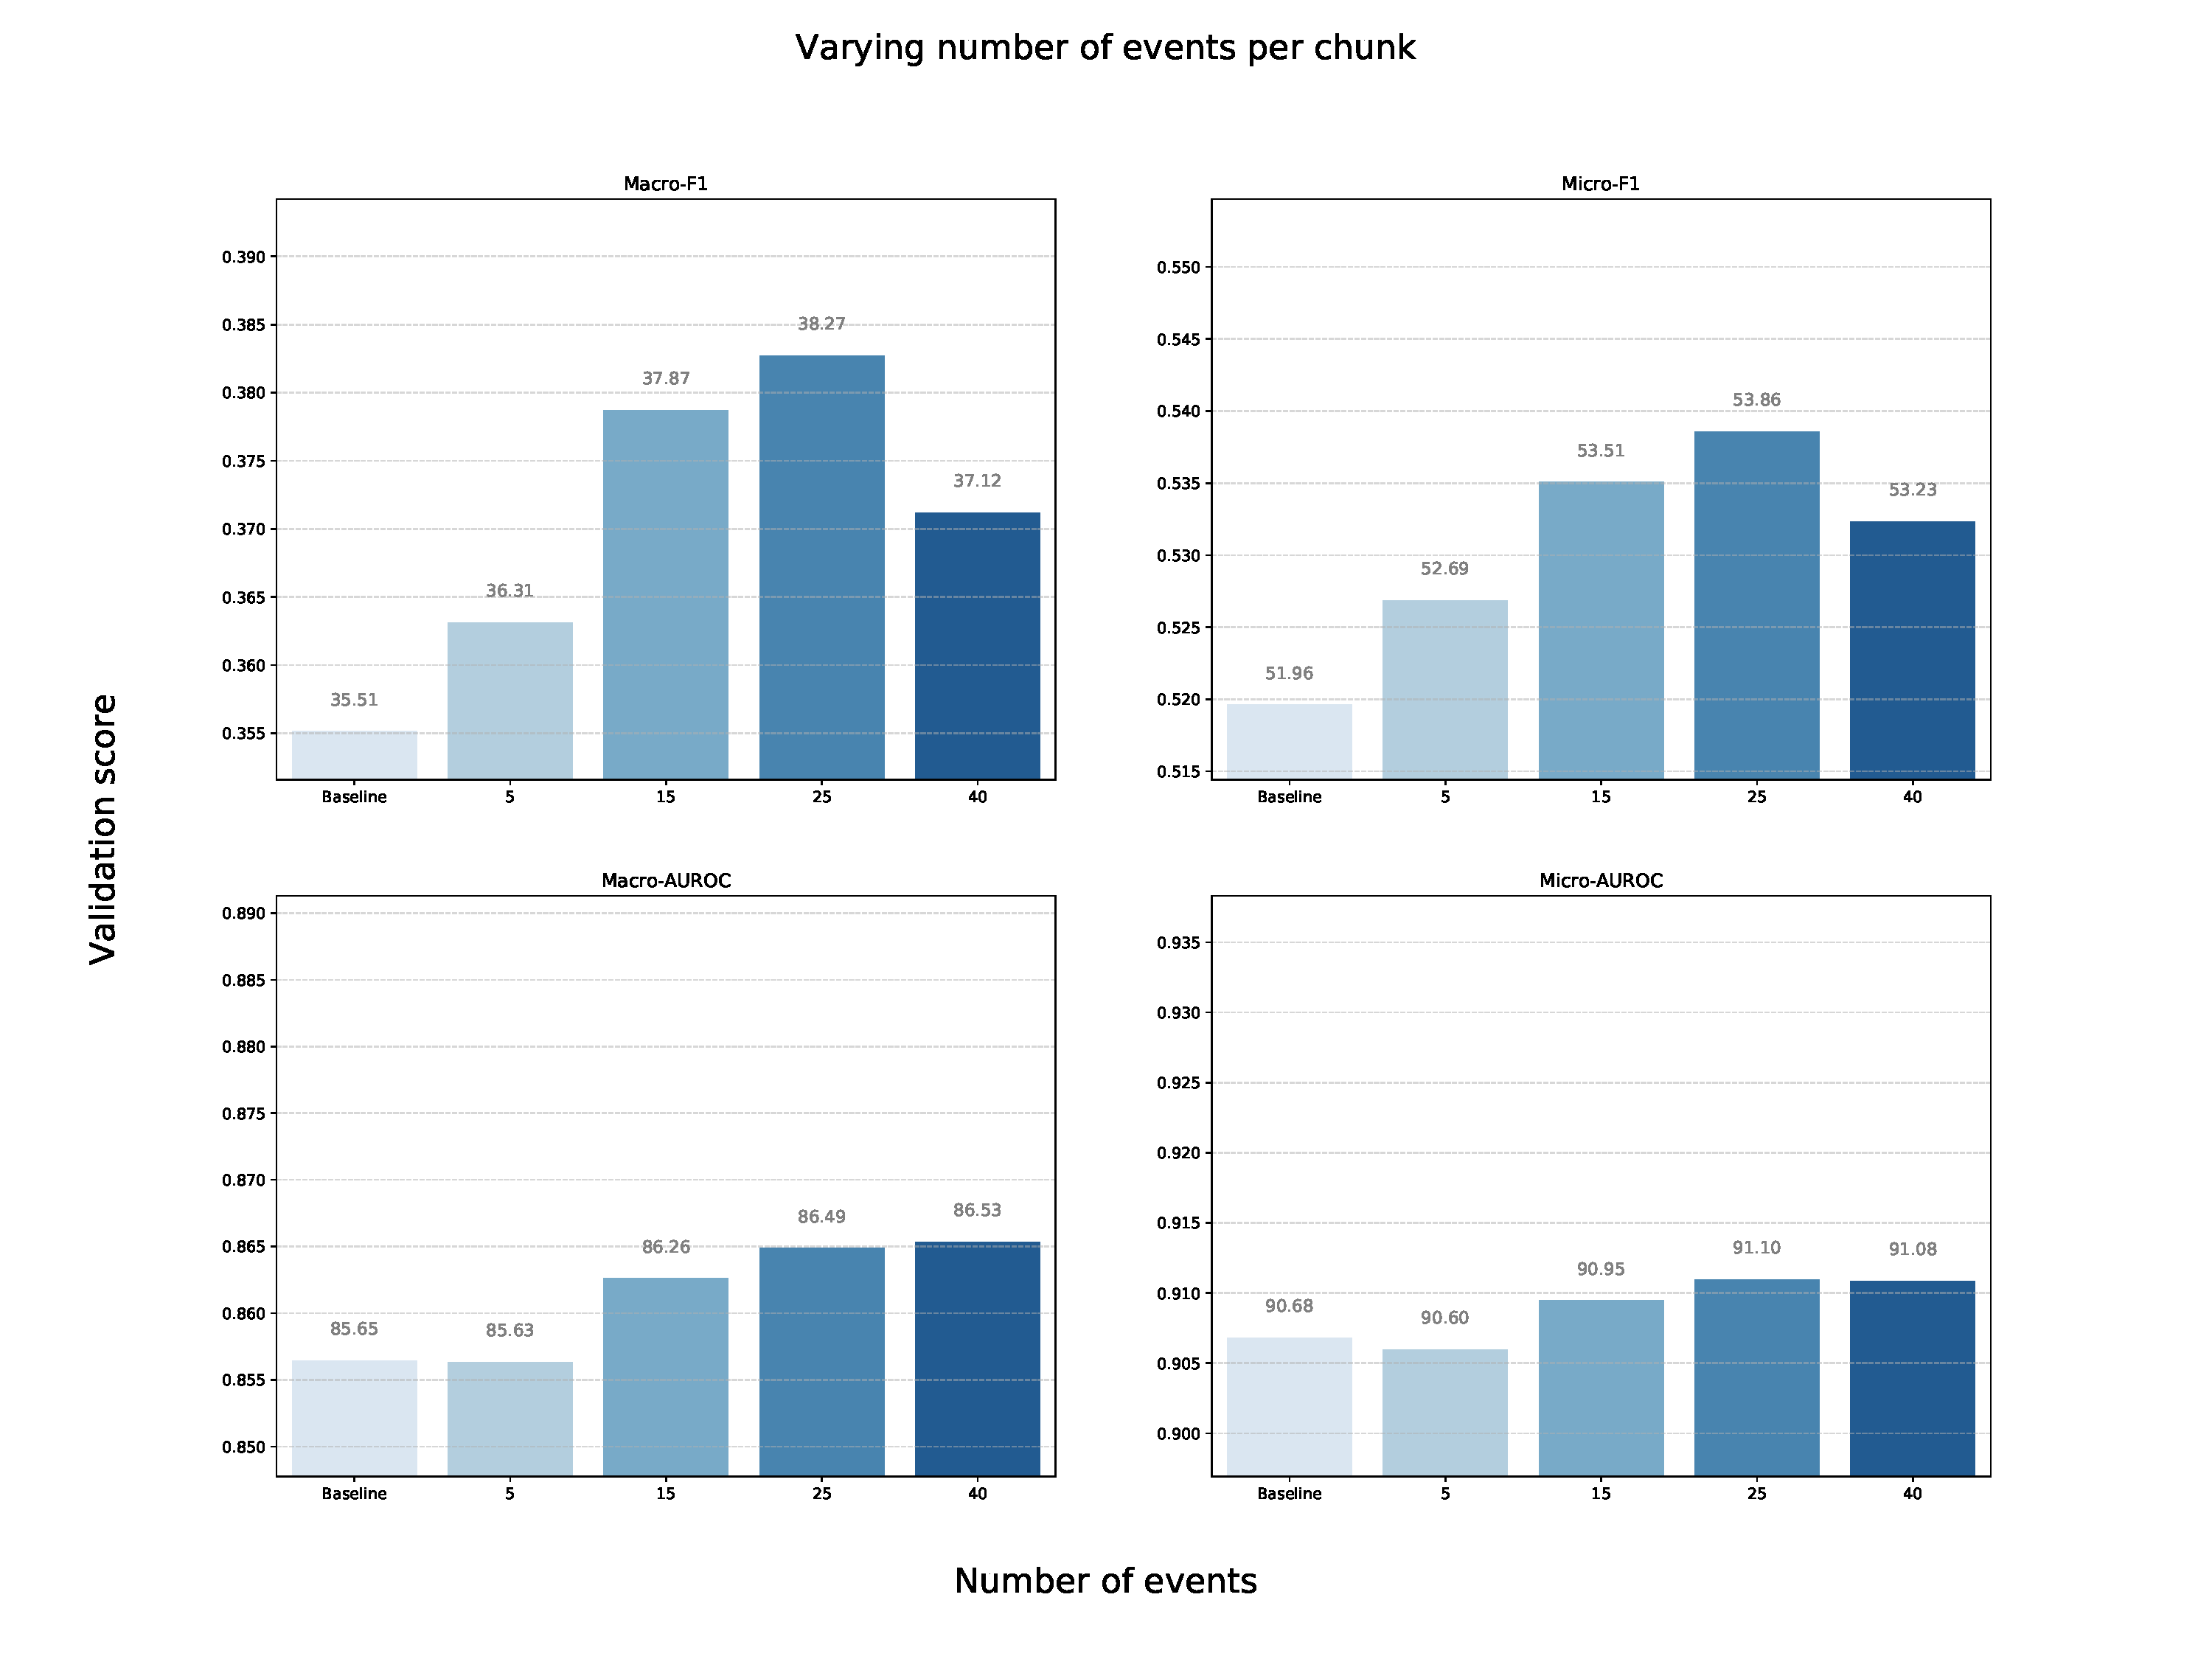
\includegraphics[width=\textwidth]{figures/exp-events.pdf}
\end{figure}
\paragraph{Discussion} As in the previous experiment, we see a clear optimum for the F1 score at 25 events per chunk and per type. Again, the conclusion is not so obvious for the AUROC score, and this metric does not seem to improve much above $K=15$.

\newpage
\subsection{Number of neighbors}
As a last experiment, we made the number of neighbors for each input entity varies. As the previous experiment, this defines the maximum number of neighbors and does not mean it will have exactly $M$ neighbors. Indeed, it is important to remember that we set a minimum \emph{WPPR} threshold of $0.0001$ that might lead to some isolated admissions having $\leq M$ neighbors.

\begin{figure}[H]
 \centering
 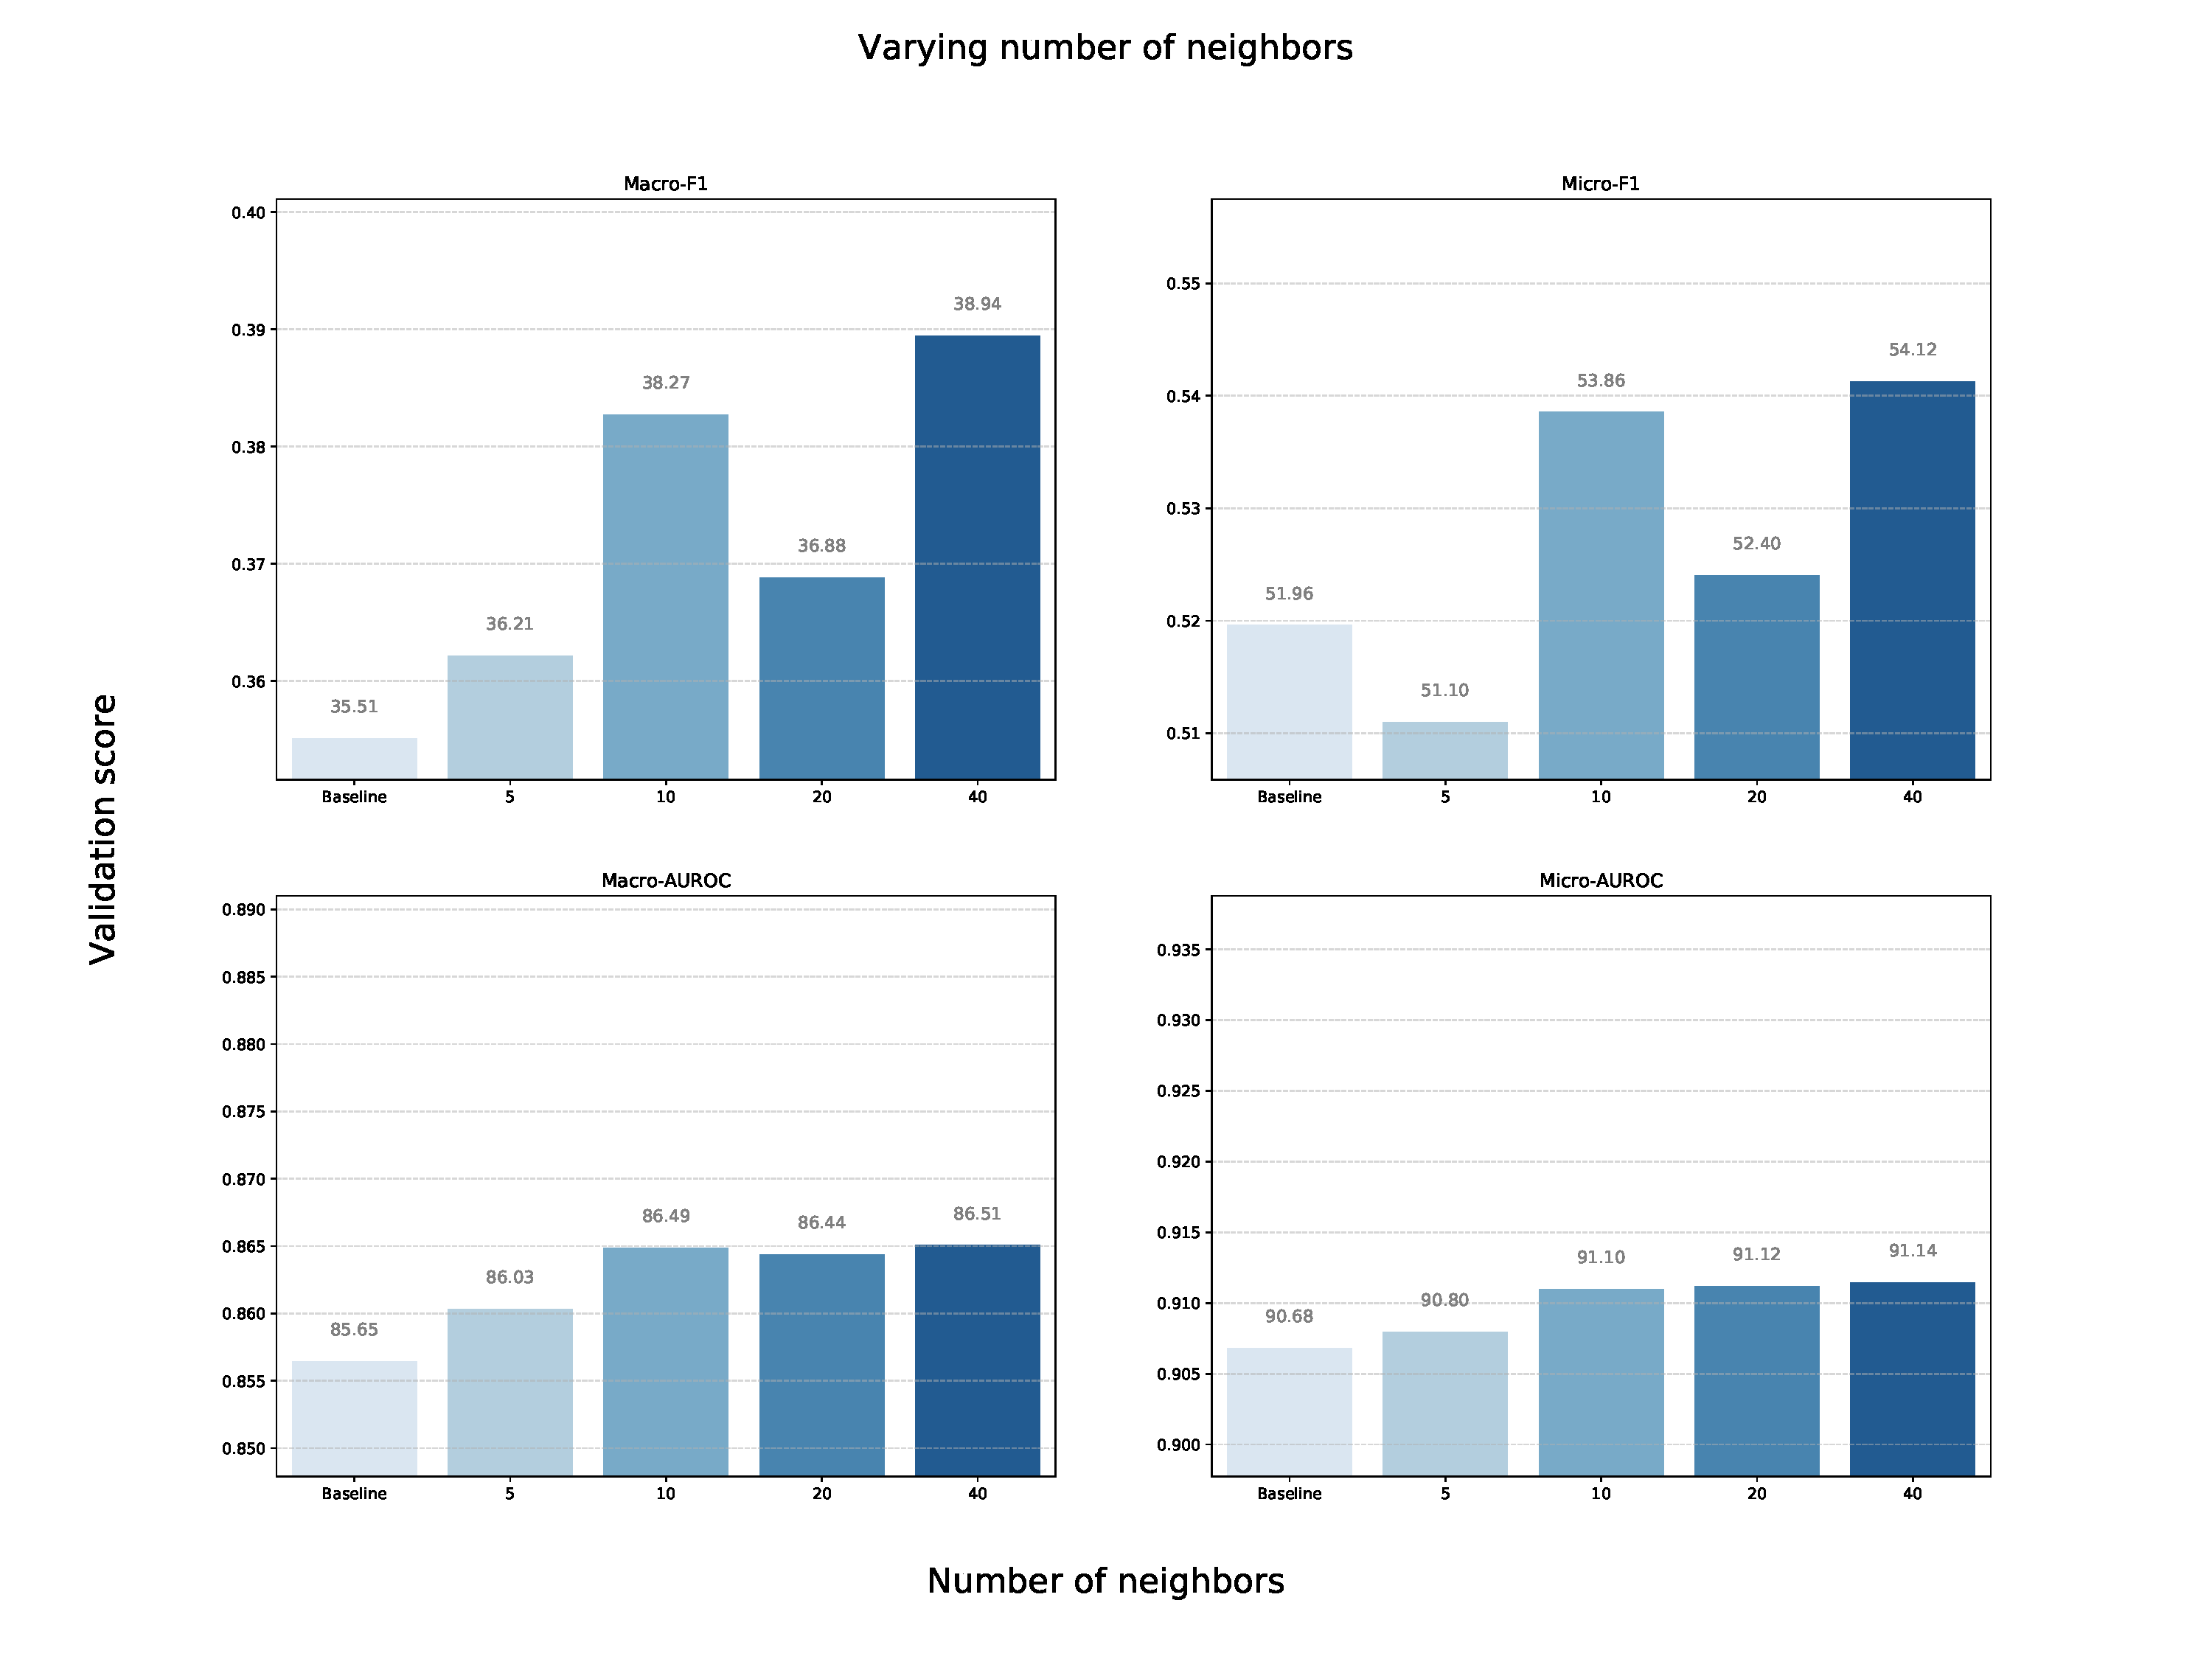
\includegraphics[width=\textwidth]{figures/exp-neighbors.pdf}
\end{figure}

\paragraph{Discussion} The results of this experiment are very interesting, yet difficult to conclude on. We can see that the number of neighbors has a huge impact on the F1 metrics, but not so much on the AUROC score. However, it is important to notice that we would expect the bar plots to have a similar shape as before. \\

That is, we would expect it to have a concave shape, where fewer neighbors means less information and thus decreased scores. Whereas, too many neighbors would add more noise than information and also hindering results. Therefore, we would expect to find an optimum value in-between but we see a drastic decrease between \textit{10} and \textit{20} neighbors, while having an increase in our metrics between \textit{20} and \textit{40} neighbors. Lastly, the scores with \textit{40} neighbors seem slightly better than with \textit{20}.

\newpage
\section{ICD9 Prediction}
\subsection{Quantitative analysis}
From these top-scoring hyper-parameters for the different groups, we selected the following parameters and ran our final evaluation for the task of predicting the top 50 ICD9 codes in a multi-class multi-classification scenario. \\

These results are all performed on the \textbf{testing set}, after all the previous hyper-parameter tuning and experiments were run on the validation set. To this end, we left the testing set untainted and the results of this section and for the task at hand will be as representative as possible from a real scenario. This testing set is made of 20\% of the dataset, totaling \textit{11'230} admissions. \\

The two following plots are interesting to compare between the baseline performances and our \emph{KG-RNN}:

\begin{figure}[H]
 \setkeys{Gin}{width=\linewidth}
 \begin{tabularx}{\textwidth}{XXXX}
  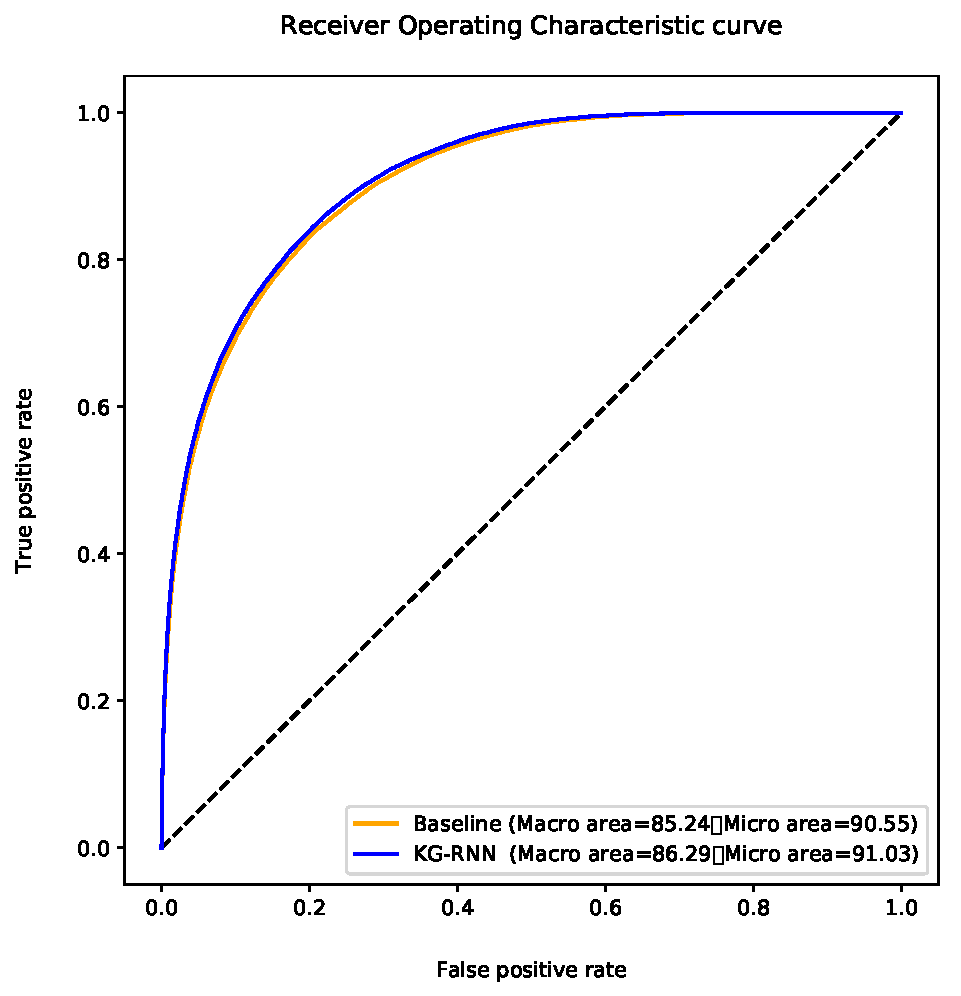
\includegraphics{figures/roc-curves.pdf} &
  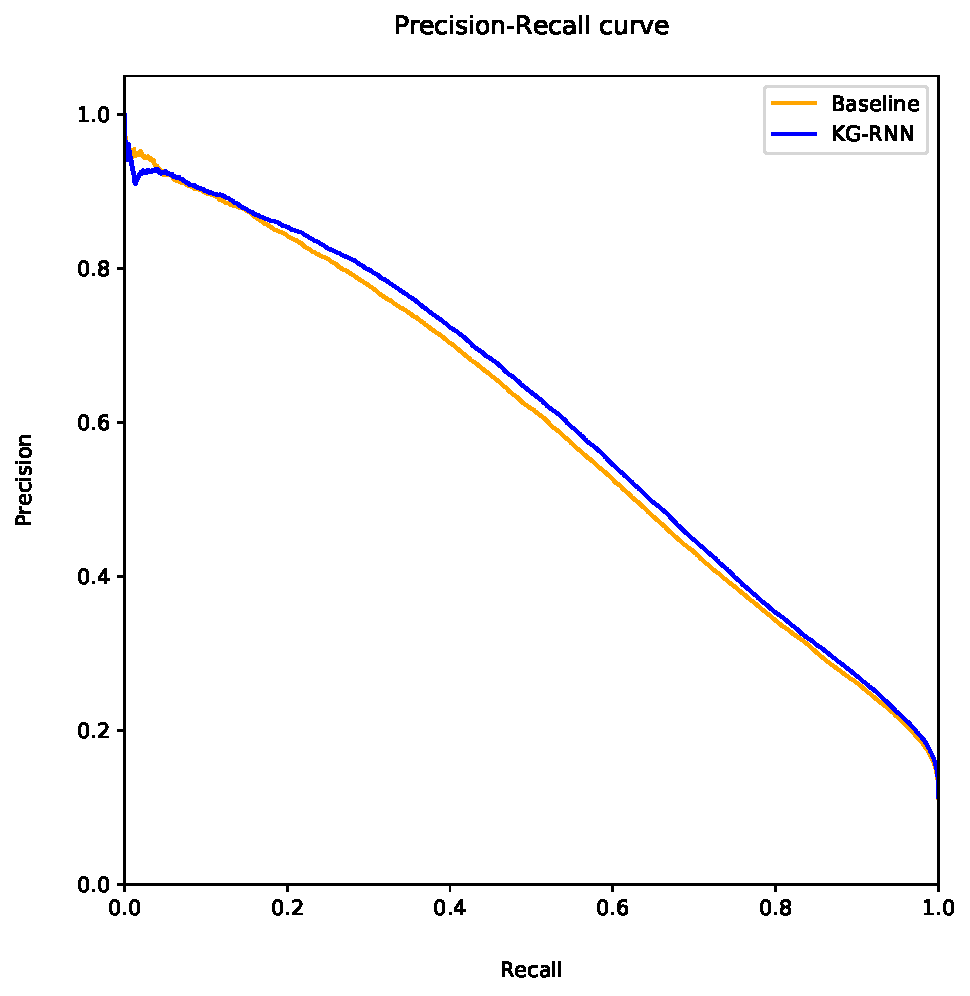
\includegraphics{figures/pr-curves.pdf}
 \end{tabularx}
 \caption{\textbf{Left}: Receiver operating characteristic curve on the testing set for both the \emph{baseline} and \emph{KG-RNN}. \textbf{Right}: Precision-recall curve on the testing set for both the \emph{baseline} and \emph{KG-RNN}.}
\end{figure}
We also evaluated the results on the different metrics that we described in the section~\ref{sec:Metrics}: \\
\begin{table}[H]
 \begin{center}
  \begin{tabular}{| p{2cm} | p{2cm} | p{2cm} | p{3cm} |}
   \hline
   &&&\\
   \textbf{Metric} & \textbf{Average} & \textbf{Model} & \textbf{Score} \\
   &&&\\ \hline
   \multirow{4}{*}{F1} & \multirow{2}{*}{Macro} & Baseline & \textbf{36.52\%} \\
   && KG-RNN & \textbf{37.90\%} (+1.38\%) \\ \cline{2-4}
   & \multirow{2}{*}{Micro} & Baseline & \textbf{51.55\%} \\
   && KG-RNN & \textbf{53.47\%} (+1.92\%) \\ \hline
   
   \multirow{4}{*}{AUROC} & \multirow{2}{*}{Macro} & Baseline & \textbf{85.24\%} \\
   && KG-RNN & \textbf{86.29\%} (+1.05\%) \\ \cline{2-4}
   & \multirow{2}{*}{Micro} & Baseline & \textbf{90.55\%} \\
   && KG-RNN & \textbf{91.03\%} (+0.48\%) \\ \hline
   
   \multirow{2}{*}{Accuracy} & \multirow{2}{*}{-} & Baseline & \textbf{92.22\%} \\
   && KG-RNN & \textbf{92.36\%} (+0.14\%) \\ \hline
  \end{tabular}
 \end{center}
\end{table}
\newpage
\paragraph{Discussion} We notice an improvement on each metric for both averages. Yet, the results are not easily distinguishable and very close to each other on the testing set compared to the validation set where the improvements from \textit{KG-RNN} were stronger. \\

To further assess the quality of our \emph{KG-RNN} model, we decided to use a statistical significance test, the McNemar's Test~\footnote{\href{https://en.wikipedia.org/wiki/McNemar\%27s\_test}{https://en.wikipedia.org/wiki/McNemar's\_test}}. Indeed, this test will allow us to get a very precise idea of the relevance of the edge that \emph{KG-RNN} seems to have over the baseline. \\

The McNemar's test requires to build a ``contingency table`` from our results, as follows: \\

\begin{table}[H]
 \begin{center}
  \begin{tabular}{ p{4cm} | p{4cm} | p{4cm} }
   & \textbf{KG-RNN is correct}  & \textbf{KG-RNN is incorrect} \\
   && \\ \hline
   && \\
   \textbf{Baseline is correct} & 510'590 (\textit{a}) & 7'247 (\textit{b}) \\
   && \\ \hline
   && \\
   \textbf{Baseline is incorrect} & 7'984 (\textit{c}) & 35'679 (\textit{d}) \\
   && \\ \hline
  \end{tabular}
 \end{center}
\end{table}

If we consider $p_b$ and $p_c$ as the theoretical cell probabilities, the null hypothesis and the alternative are:

\begin{equation*}
 \begin{aligned}
  H_0: &&p_b = p_c \\
  H_1: &&p_b \neq p_c
 \end{aligned}
\end{equation*}

In other words, \textbf{under the null hypothesis, the two models should have the same error rate.} and we can summarize this as follows:

\begin{itemize}
 \item \textbf{Fail to Reject Null Hypothesis}: Classifiers have a similar proportion of errors on the testing set.
 \item \textbf{Reject Null Hypothesis}: Classifiers have a different proportion of errors on the testing set.
\end{itemize}

Where under the null hypothesis and with a sufficient amount of data (which is our case), the statistic should follow a chi-squared distribution with 1 degree of freedom. \\

Notably, in our case the \emph{Corrected McNemar} test statistic is: \\

\begin{equation}
\chi^2 = \frac{(|b-c|-1)^2}{b+c} = \frac{(|7247-7984|-1)^2}{7247+7984} = 35.57
\end{equation}

and the associated \textbf{p-value} under $H_0$ is $P=0.0000000025$, which is extremely small and statistically significant. \\

Hence, our p-value shows sufficient evidence to reject the null in favor of the alternative hypothesis. Therefore, the two models have different performances when trained on this particular testing set, supporting the idea that the edge over the baseline is not due to randomness but rather a truly improved predictive power.

\newpage
\subsection{Qualitative Analysis}
\label{subsec:Qualitative analysis}
\paragraph{Embeddings} First off, we decided to analyze the embedding we optimized while training \emph{KG-RNN}. For this purpose, we projected our embedding matrices into two dimensions using a Uniform Manifold Approximation and Projection~\cite{2018arXivUMAP}. Then, we picked a laboratory measurement (\textbf{White Blood Cells}) and a prescription (\textbf{Sodium}) to extract their nearest neighbors in the projected 2D manifold:
\begin{multicols}{2}
 \centering
 Neighbors for \textbf{White Blood Cells}
 \begin{center}
  \begin{tabular}{| c | c |}
   \hline
   \textbf{Rank} & \textbf{Laboratory measure} \\ \hline
   1 & WBC \\ \hline
   3 & White Cells \\ \hline
   6 & Immunoglobulin A \\
   \hline
  \end{tabular}
 \end{center}\columnbreak
 \vfill
 Neighbors for \textbf{Sodium}
 \begin{center}
  \begin{tabular}{| c | c |}
   \hline
   \textbf{Rank} & \textbf{Prescription} \\ \hline
   1 & Sodium Chloride Nasal \\ \hline
   2 & Sodium Chloride 0.9\%  Flush \\ \hline
   5 & Famotidine \\
   \hline
  \end{tabular}
 \end{center}
\end{multicols}

In the first case (i.e. \textit{White Blood Cells}), it is very interesting to notice that among the neighbors, we first find an abbreviation of the same laboratory measurement: \textbf{WBC}, as well as a short name of it at the third-closest neighbor: \textbf{White Cells}. Finally, we also see the compelling evidence that the embedding is of good quality by the positioning of \textbf{Immunoglobulin A}, which are antibodies produced by white blood cells. \\

In the second table, we see that \textit{Sodium} is close to its related prescriptions in the first two nearest neighbors. Whereas, \textbf{Famotidine} is also ranked very close at the fifth rank, and it is known in the medical field that Famotidine is often given in \textbf{0.9\% Sodium Chloride} through intravenous, our second neighbor. \\

Overall, we can see with these two examples that \emph{KG-RNN} has not only learned similar events, such as ``White Blood Cells`` and ``WBC``, but also intrinsically and correlated linked events. Indeed, as we noticed, our deep learning architecture mapped events close to each other in the embedding space if they are related in the medical domain, learning more complex interactions.

\newpage
\paragraph{Predictions} Secondly, to have a better understanding of the value provided by \emph{KG-RNN} over the baseline, we extracted a few samples where the baseline was incorrect but KG-RNN was right in its prediction (represented by \textit{c} in the ``contingency table``). \\

From the extracted samples and to the purpose of understanding the differences, we also checked the information conveyed by neighbors of the input admission. To this end, we are able to analyze and visualize where the correctness of \emph{KG-RNN} over the baseline comes from. \\

In the following graphs, the first row corresponds to the input admission while the other ones to its neighbors. Each red line shows an ICD9 code actually diagnosed at discharge (i.e. the ground truth), and the horizontal gray line represents the default 0.5 threshold above which a prediction is considered.  In the input admission graph (first row), the orange and blue bars are the estimated probabilities by the models, respectively the baseline and \emph{KG-RNN}. Finally, in the neighbor rows, the dark-gray bars represent their final diagnoses (i.e. entity static information) as one-hot vectors. \\

\begin{figure}[H]
 \centering
 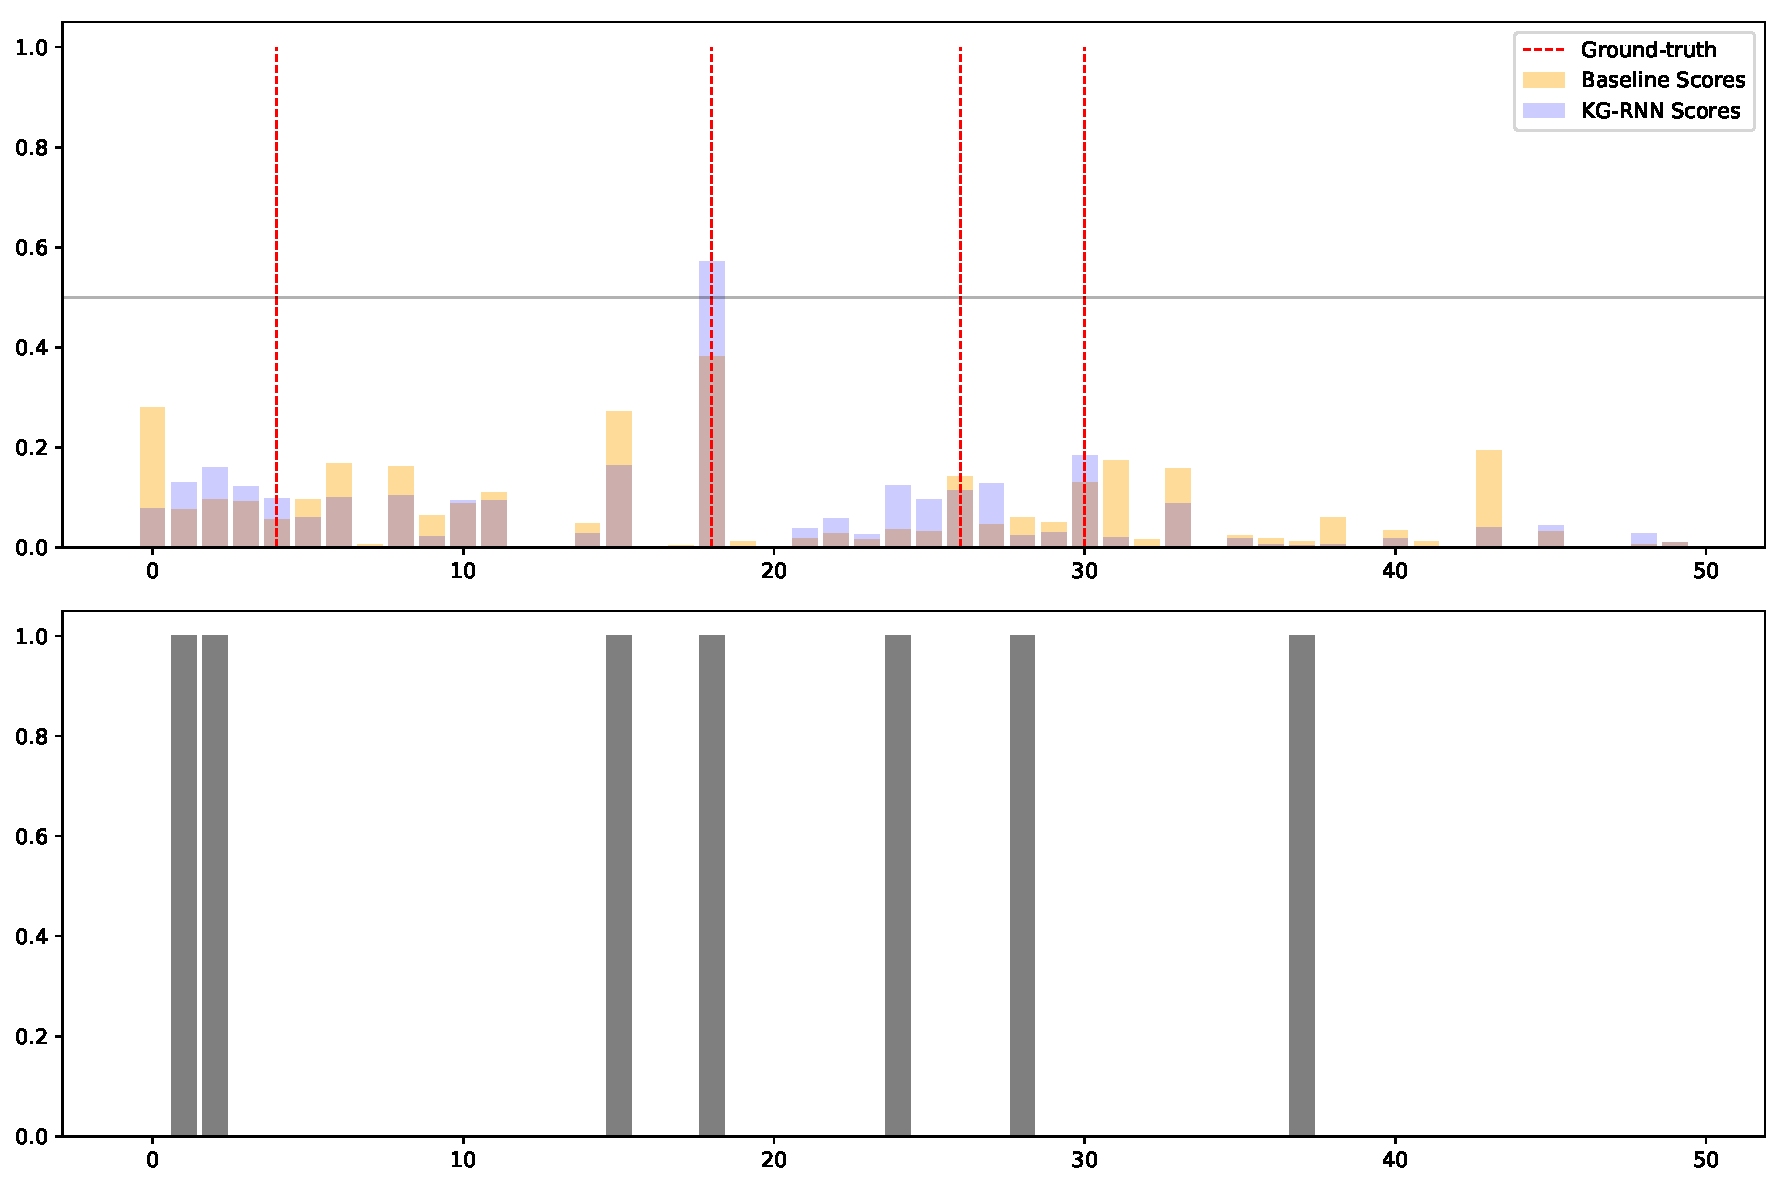
\includegraphics[width=0.8\textwidth]{figures/preds-0.pdf}
 \caption{In this plot we can see that the neighbors provide the necessary information to \emph{KG-RNN} to improve over the baseline. Indeed, this model does not detect any diagnostic, whereas KG-RNN is able to predict the second one with the help of its neighbor. Namely, we hypothesize that since its neighbor static information conveys the ICD9 code of interest (the second one), it helped pushing the confidence of KG-RNN upward, above the 0.5 decision threshold.}
\end{figure}

\newpage
The ICD9 codes of the ground truth and the neighbor from the previous figure are summarized in the following table:

\begin{table}[H]
 \begin{center}
  \textbf{Input admission} \\
  
  \begin{tabular}{| c | c | p{8cm} |}
   \hline
   \textbf{Rank} & \textbf{ICD9 Code} & \textbf{Description} \\ \hline
   4 & 272.4 & Other and unspecified hyperlipidemia  \\ \hline
   18 & 401.9 & Unspecified essential hypertension \\ \hline
   26 & 486 & Pneumonia, organism unspecified \\ \hline
   30 & 530.81 & Esophageal reflux \\ \hline
  \end{tabular}
 \end{center}
\end{table}
\begin{table}[H]
 \begin{center}
  \textbf{Neighbor} \\
  
  \begin{tabular}{| c | c | p{8cm} |}
   \hline
   \textbf{Rank} & \textbf{ICD9 Code} & \textbf{Description} \\ \hline
   1 & 244.9 & Unspecified acquired hypothyroidism \\ \hline
   2 & 250.00 & Diabetes mellitus without mention of complication, type II or unspecified type, not stated as uncontrolled \\ \hline
   15 & 38.93 & Unspecified septicemia \\ \hline
   18 & 401.9 & Unspecified essential hypertension \\ \hline
   24 & 427.31 & Atrial fibrillation \\ \hline
   28 & 507.0 & Pneumonitis due to inhalation of food or vomitus \\ \hline
   37 & 96.6 & Late syphilis, latent \\ \hline
  \end{tabular}
 \end{center}
\end{table}

It is interesting to see that even if the neighbor diagnoses do not match the ground truth \textit{perfectly}, some ICD9 codes still convey information for the input admission. Indeed, if we look at the number \textbf{26} in the input admission (i.e. \textit{Pneumonia}), it could be linked to the number \textbf{28} of the neighbor (i.e. \textit{Pneumonitis}). However, even if the final diagnoses are different (``Pneumonitis`` indicates inflammation of lung tissues, whereas ``Pneumonia`` is inflammation caused by an infection), the admissions are linked through their pre-diagnosis and thus one may carry information on the other. \\

Therefore, using the ICD9 code hierarchy may help the model to make sense from neighbors diagnoses and increase predictive power for the input admission. This potential trail is further described in the appropriate section~\ref{sec:Future Work} of the last chapter.

\newpage
\begin{figure}[H]
 \centering
 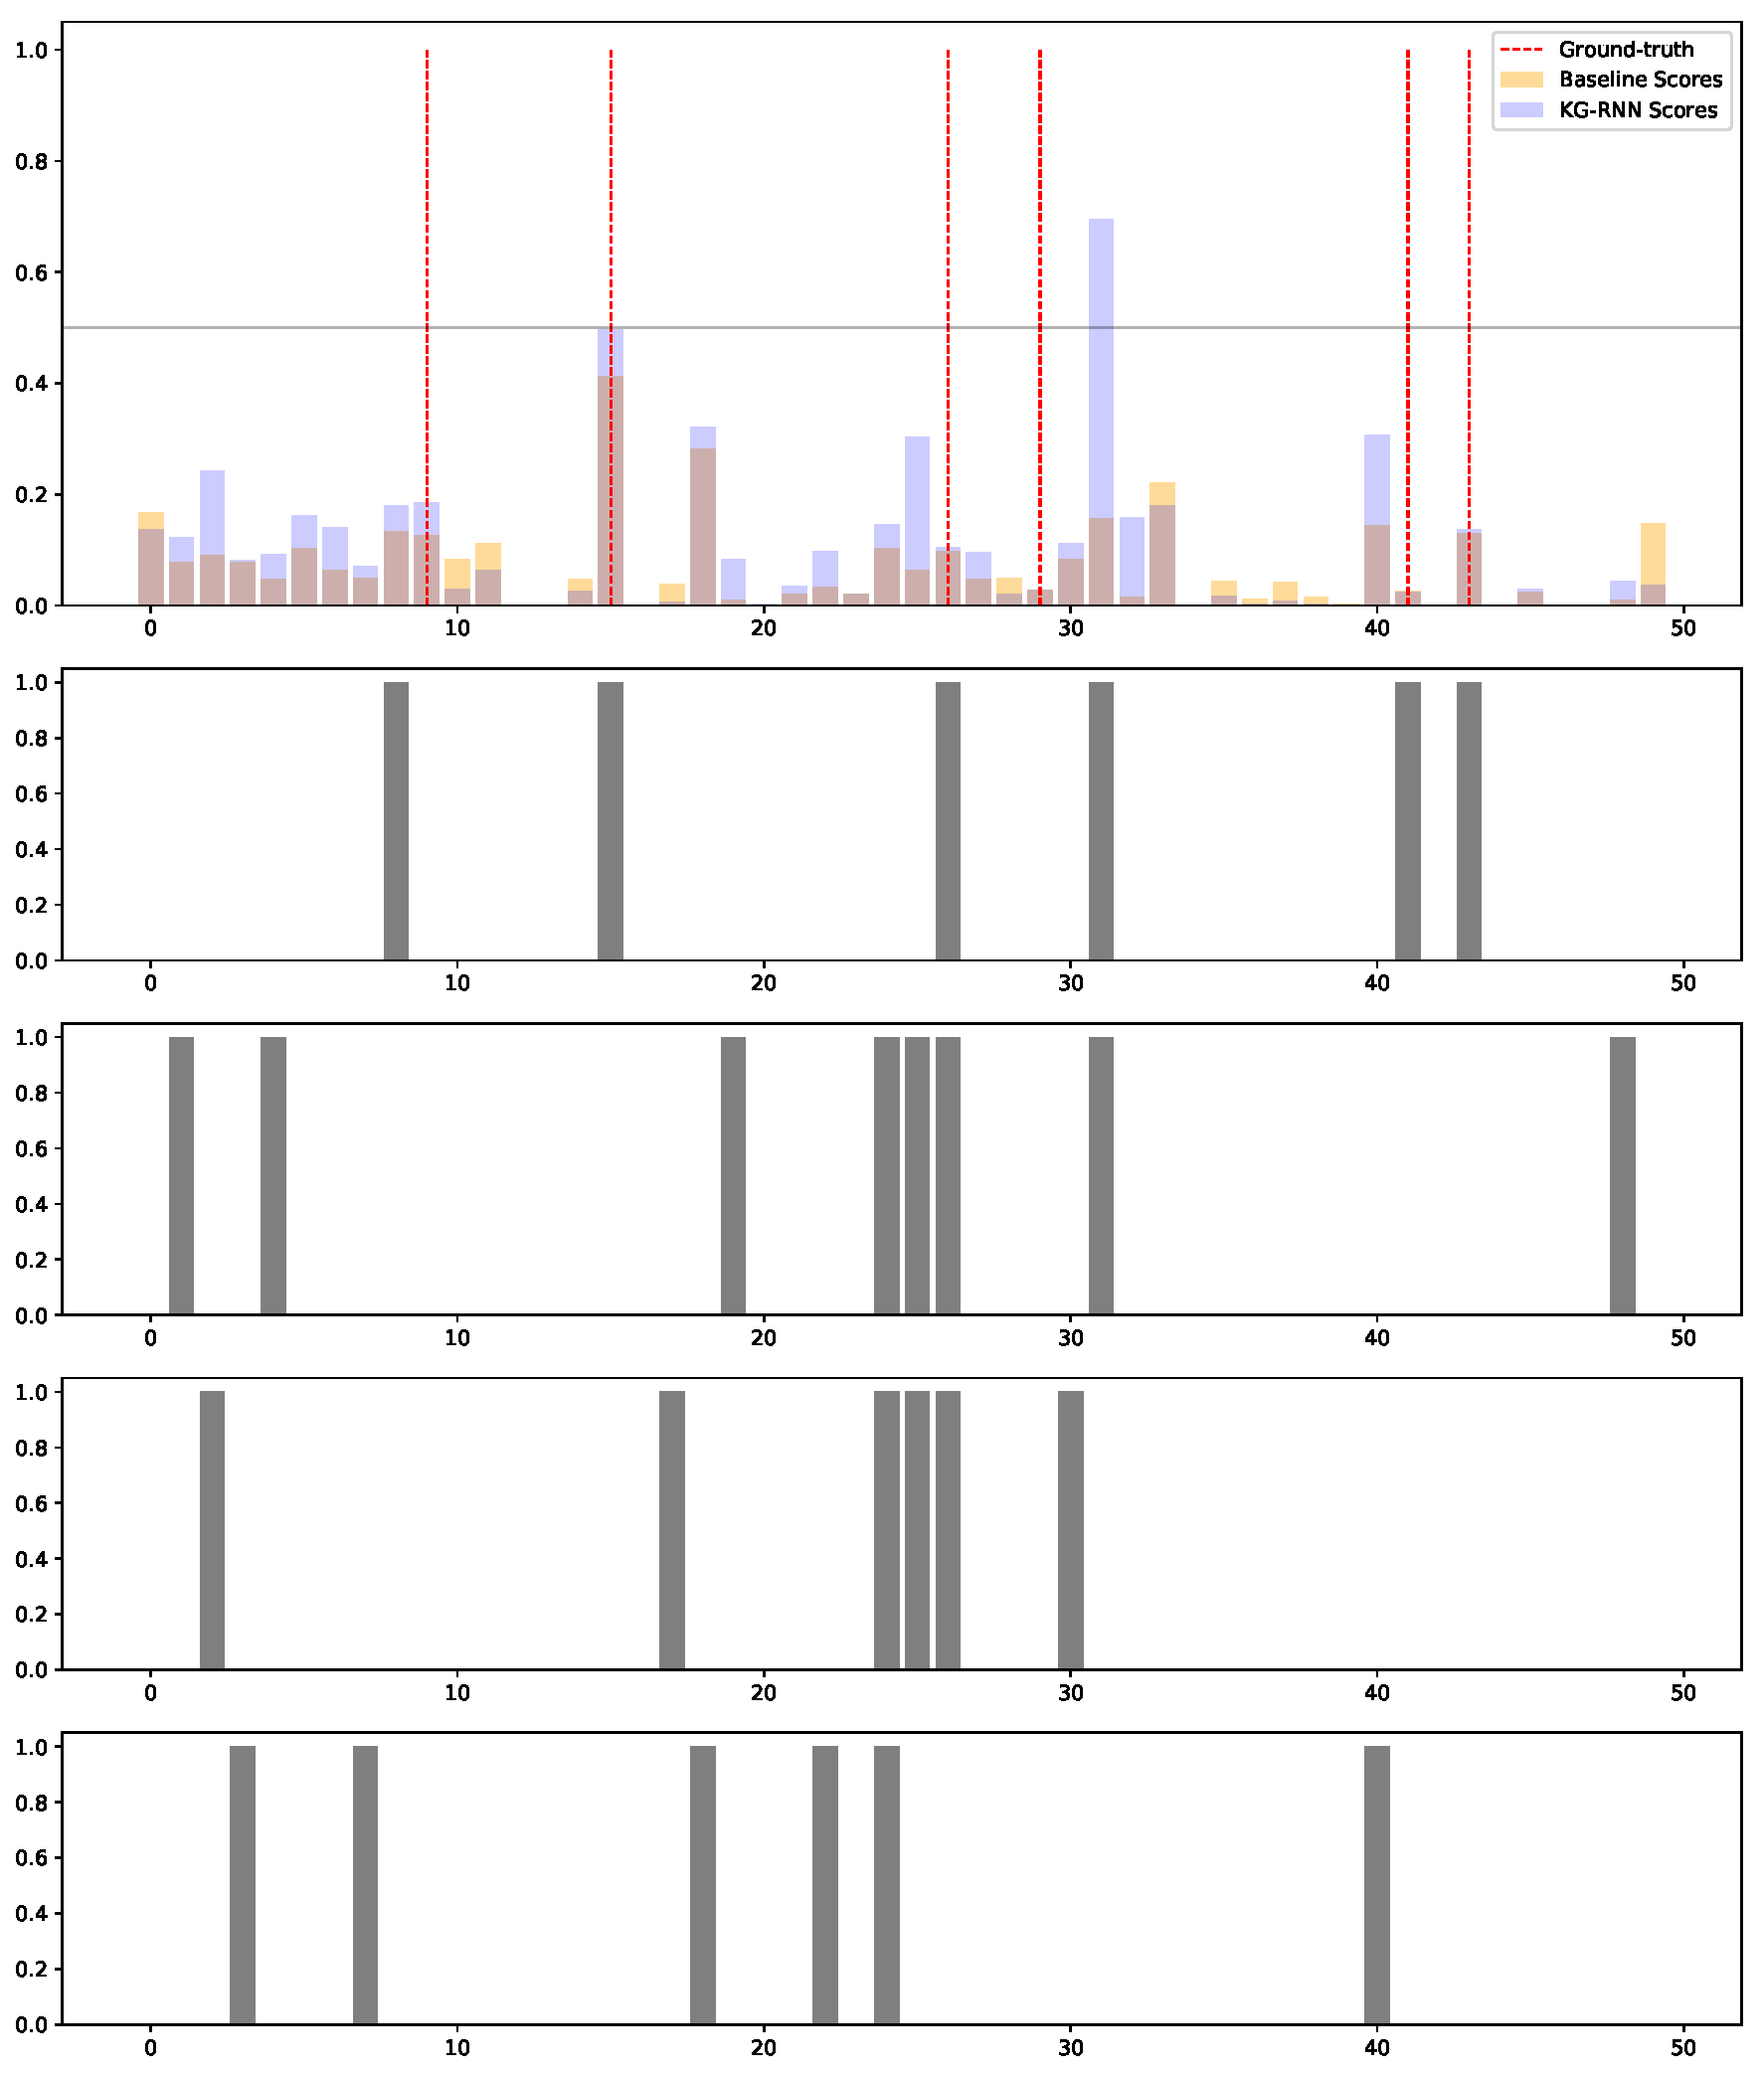
\includegraphics[width=0.8\textwidth]{figures/preds-1.pdf}
 \caption{In this plot, the input admission has 4 neighbors with different final diagnoses (static information), and we also notice interesting behavior of \emph{KG-RNN} compared to the baseline. In this scenario, we see that the first neighbor helps pushing the confidence of the model over the decision threshold for the second diagnosed ICD9 code. However, we also see that \emph{KG-RNN} is misled by the first two neighbors that are wrongly pushing ICD9 number thirty-one over the decision threshold. This highlights the importance of a good knowledge graph construction and neighbors extraction algorithm.}
\end{figure}

To conclude, we see that neighbors are having a big impact on KG-RNN, as the predictions where $\mbox{Score}_{\mbox{baseline}} \ge \mbox{Score}_{\mbox{KG-RNN}}$ occur when none of the neighbors have a matching ICD9 code. On the other hand, when one or more of the neighbors have a certain ICD9 code, the corresponding score for \emph{KG-RNN} on the input admission is consistently pushed upwards. This reveals how much KG-RNN learns to rely on its neighbors to score its predictions.
\chapter{Concluding Remarks}
\label{chap:Concluding Remarks}
In this concluding chapter, we first go through a conclusion of the work presented in this thesis, in the section~\ref{sec:Conclusion}. We summarize our results and discuss the potential answer to the questions in the section~\ref{sec:Research Question & Contributions}. \\

Finally, we elaborate on some potential trails for future work and how the current version of \emph{KG-RNN} could be improved. Each idea of possible improvement is described briefly in a separate paragraph and were not implemented mostly due to time constraints.

\section{Conclusion}
\label{sec:Conclusion}
In this thesis, we proposed a novel architecture and pipeline for processing evolving knowledge graphs. This architecture has shown to exploit well information from other entities, through complex linkage structure created with external data sources. \\

For our specific use-case in health-science, our enriched knowledge graph has been processed to naturally cope with many of the challenges inherent to the application. In particular, we proposed a way to create \textit{patient states} from the knowledge graph that can be seen as \textit{graph states} and further fed into our KG-RNN pipeline. \\

In this scenario of predicting the top-50 diagnoses at discharge, our solution shows significant improvement over a simple single-admission setting. We evaluated our results both quantitatively and qualitatively to understand the pros and cons of the approach. These bottlenecks helped suggest further improvements that could be experimented to design a better second version of the \emph{KG-RNN} pipeline. \\

Lastly, it would be very insightful to test our architecture on other use-cases in order to cross-validate qualitative and quantitative performances. More over, understanding the role of the different hyper-parameters and their impact on other use-cases could lead to beneficial insights for future versions of the pipeline.

\newpage
\section{Future Work}
\label{sec:Future Work}
As explained previously, this section is subdivided in paragraphs that each explains a potential improvement over our proposed pipeline. \\

These suggestions are not ordered in terms of priority and may be implemented in whatever order the reader prefers, as they are all independent from each other.

\paragraph{Knowledge Graph Extensions}
The first and most obvious improvement lies in adding external sources to our knowledge graph to enrich the information it may carry. We hypothesize that our \textit{Weighted Personalized PageRank} approach scales well and makes even more sense for complex linkage structures. \\

This improvement may lead to important changes in the different metrics as our KG-RNN pipeline seems to leverage the knowledge graph information.

\paragraph{Events sampler}
Within the data formation section~\ref{sec:Formation}, we describe that if the number of events in a given chunk for a certain type exceeds $K$, we randomly sample those. \\

A potential improvement would be to use a more advanced sampling techniques to down-sample events with respect to their importance. Indeed, some events might carry more information for the final diagnoses than others and they could be discarded by \textit{blindly} sampling randomly among them.

\paragraph{Neighbors Weighting}
In the current pipeline proposal, all neighbors are considered of equal importance. However, this assumption is incorrect as some may be more relevant than others with respect to the input admission. \\

To account for neighbor importance, one could use the WPPR score as a weighting coefficient for each neighbor, in front of the encoding vector, for example. However, this improvement will be more relevant as the knowledge graph structure complexity increases, leading to disparate coefficients, as with the current knowledge graph they are pretty uniforms among sampled neighbors.

\paragraph{Smarter Hyper-Optimization}
A better hyper-parameter optimization is a very interesting low-hanging fruit to explore. Indeed, given the number of hyper-parameters and limited computational power as well as time constraints, a simple random search is likely to miss top-scoring configurations. \\

On the other hand, something like ``Bayesian optimization`` or ``TPE optimization`` could be smarter in how they explore the hyper-parameter space and find a better setting much faster. This improvement would be very easily implemented and is independent from models or pipeline improvements.

\paragraph{Distance-based Aggregators}
If we increase the number of sources of information for the knowledge graph, its complexity will inherently increase. That is, the WPPR-based sampling will most likely sample neighbors at different hop distance. \\

In that regard, it may be interesting to adopt a strategy like GraphSAGE~\cite{DBLP:journals/corr/HamiltonYL17} which builds a different aggregator for each hop distance. This strategy could be easily coupled with our approach to have a different aggregator for each entity type (i.e. event type).

\paragraph{Threshold Tuning}
For any practical application, the final threshold to pass before triggering an alert is a critical parameter. Indeed, this threshold is very application dependent and rules the precision vs. recall trade-off. \\

This threshold tuning could be automated or semi-automated by using a testing set to define the optimal threshold given precision or recall level we would like to reach.

\paragraph{Chunks Overlap}
During the data preparation described in section~\ref{sec:Preparation}, we could have an additional parameter to calibrate how much overlap there should be between two consecutive chunks. Currently, the KG-RNN pipeline does not add any overlap between chunks and they are perfectly disjoint and defined by $\tau$. \\

However, overlapping patient states may convey more and smoother information than disjoint ones, at the cost of adding an additional hyper-parameter (that could be trivially set to $\tau/2$). We argue that this need of overlapping chunks vs. disjoint ones is application dependent and hence a hyper-parameter may suit better to test different configurations for the task at hand.

\paragraph{ICD9 Hierarchy}
As a last second application dependent improvement (on top of ``Admissions Chunking``), and as discussed in the qualitative study of our results in subsection~\ref{subsec:Qualitative analysis}, it would be very valuable to account for medical domain knowledge. In that purpose, leveraging information from the ICD9 hierarchy could lead to improved results and interpretability of neighbors. \\

Indeed, in the current version of the knowledge graph, two neighbors are indirectly linked together through their pre-diagnosis. This information may be similar between two admissions but lead to different diagnoses. However the current architecture does not account for \textbf{diagnoses distance}. As an example, \textit{Pneumonia} and \textit{Pneumonitis} are probably ``closer`` in relevance than \textit{Pneumonia} and \textit{Diabetes}, and the ICD9 hierarchy may help to convey this kind of information with some tree-based distance. Practically, distances between diagnoses could be incorporated in the knowledge graphs by creating additional links between admissions, weighted by their distance in the ICD9 hierarchy. \\

In a similar fashion, the loss could be adapted to decrease impact of errors where the distance within the tree is smaller. As an example, the two codes ``401.9`` and  ``401.8`` are harder to distinguish than ``401.9`` and ``507.8``, and thus the model should be less \textit{punished} for mistaking the first two.

%% ----------------------------------------------------------------
\bibliographystyle{ieeetr}
\bibliography{references}

%\thesisappendix
%\thesisbib
\begin{appendices}
	%\chapter{Test}
\section{Section}
\subsection{Subsection}
\paragraph{Paragraph}

%TODO: Proof that PPR = Random Walk - https://stats.stackexchange.com/questions/258306/random-walk-with-restart-vs-personalized-pagerank
%TODO: Results of random search
%TODO: What has been tried and did not work 
\end{appendices}

%% ----------------------------------------------------------------
%\thesisback
%\input{./Back/DeclarationOfAuthorship}
%% ----------------------------------------------------------------
\end{document}
%% ----------------------------------------------------------------
